\documentclass[journal]{IEEEtran}
\usepackage[a5paper, margin=10mm]{geometry}
\usepackage{tfrupee} % Include tfrupee package

\setlength{\headheight}{1cm} % Set the height of the header box
\setlength{\headsep}{0mm}     % Set the distance between the header box and the top of the text

\usepackage{gvv-book}
\usepackage{gvv}
\usetikzlibrary{patterns}
\lstset{aboveskip=12pt}
\usepackage[center]{caption}
\raggedbottom
\setlength{\multicolsep}{0pt}

\hypersetup{
    colorlinks=true,
    urlcolor=black % Changes text color instead of placing a box around it
}
\usepackage{amsfonts}
\makeindex

\begin{document}
\bibliographystyle{IEEEtran}
\onecolumn

\title{CBSE 2018 Mathematics\\Class 10 and Class 12 Question Papers\\
\large Math for EE\\[-0.5em]
\rule{0.4\columnwidth}{0.4pt}
}

\author{Vishweshwar - ee26btech11225
\vspace{10cm}
\begin{center}
    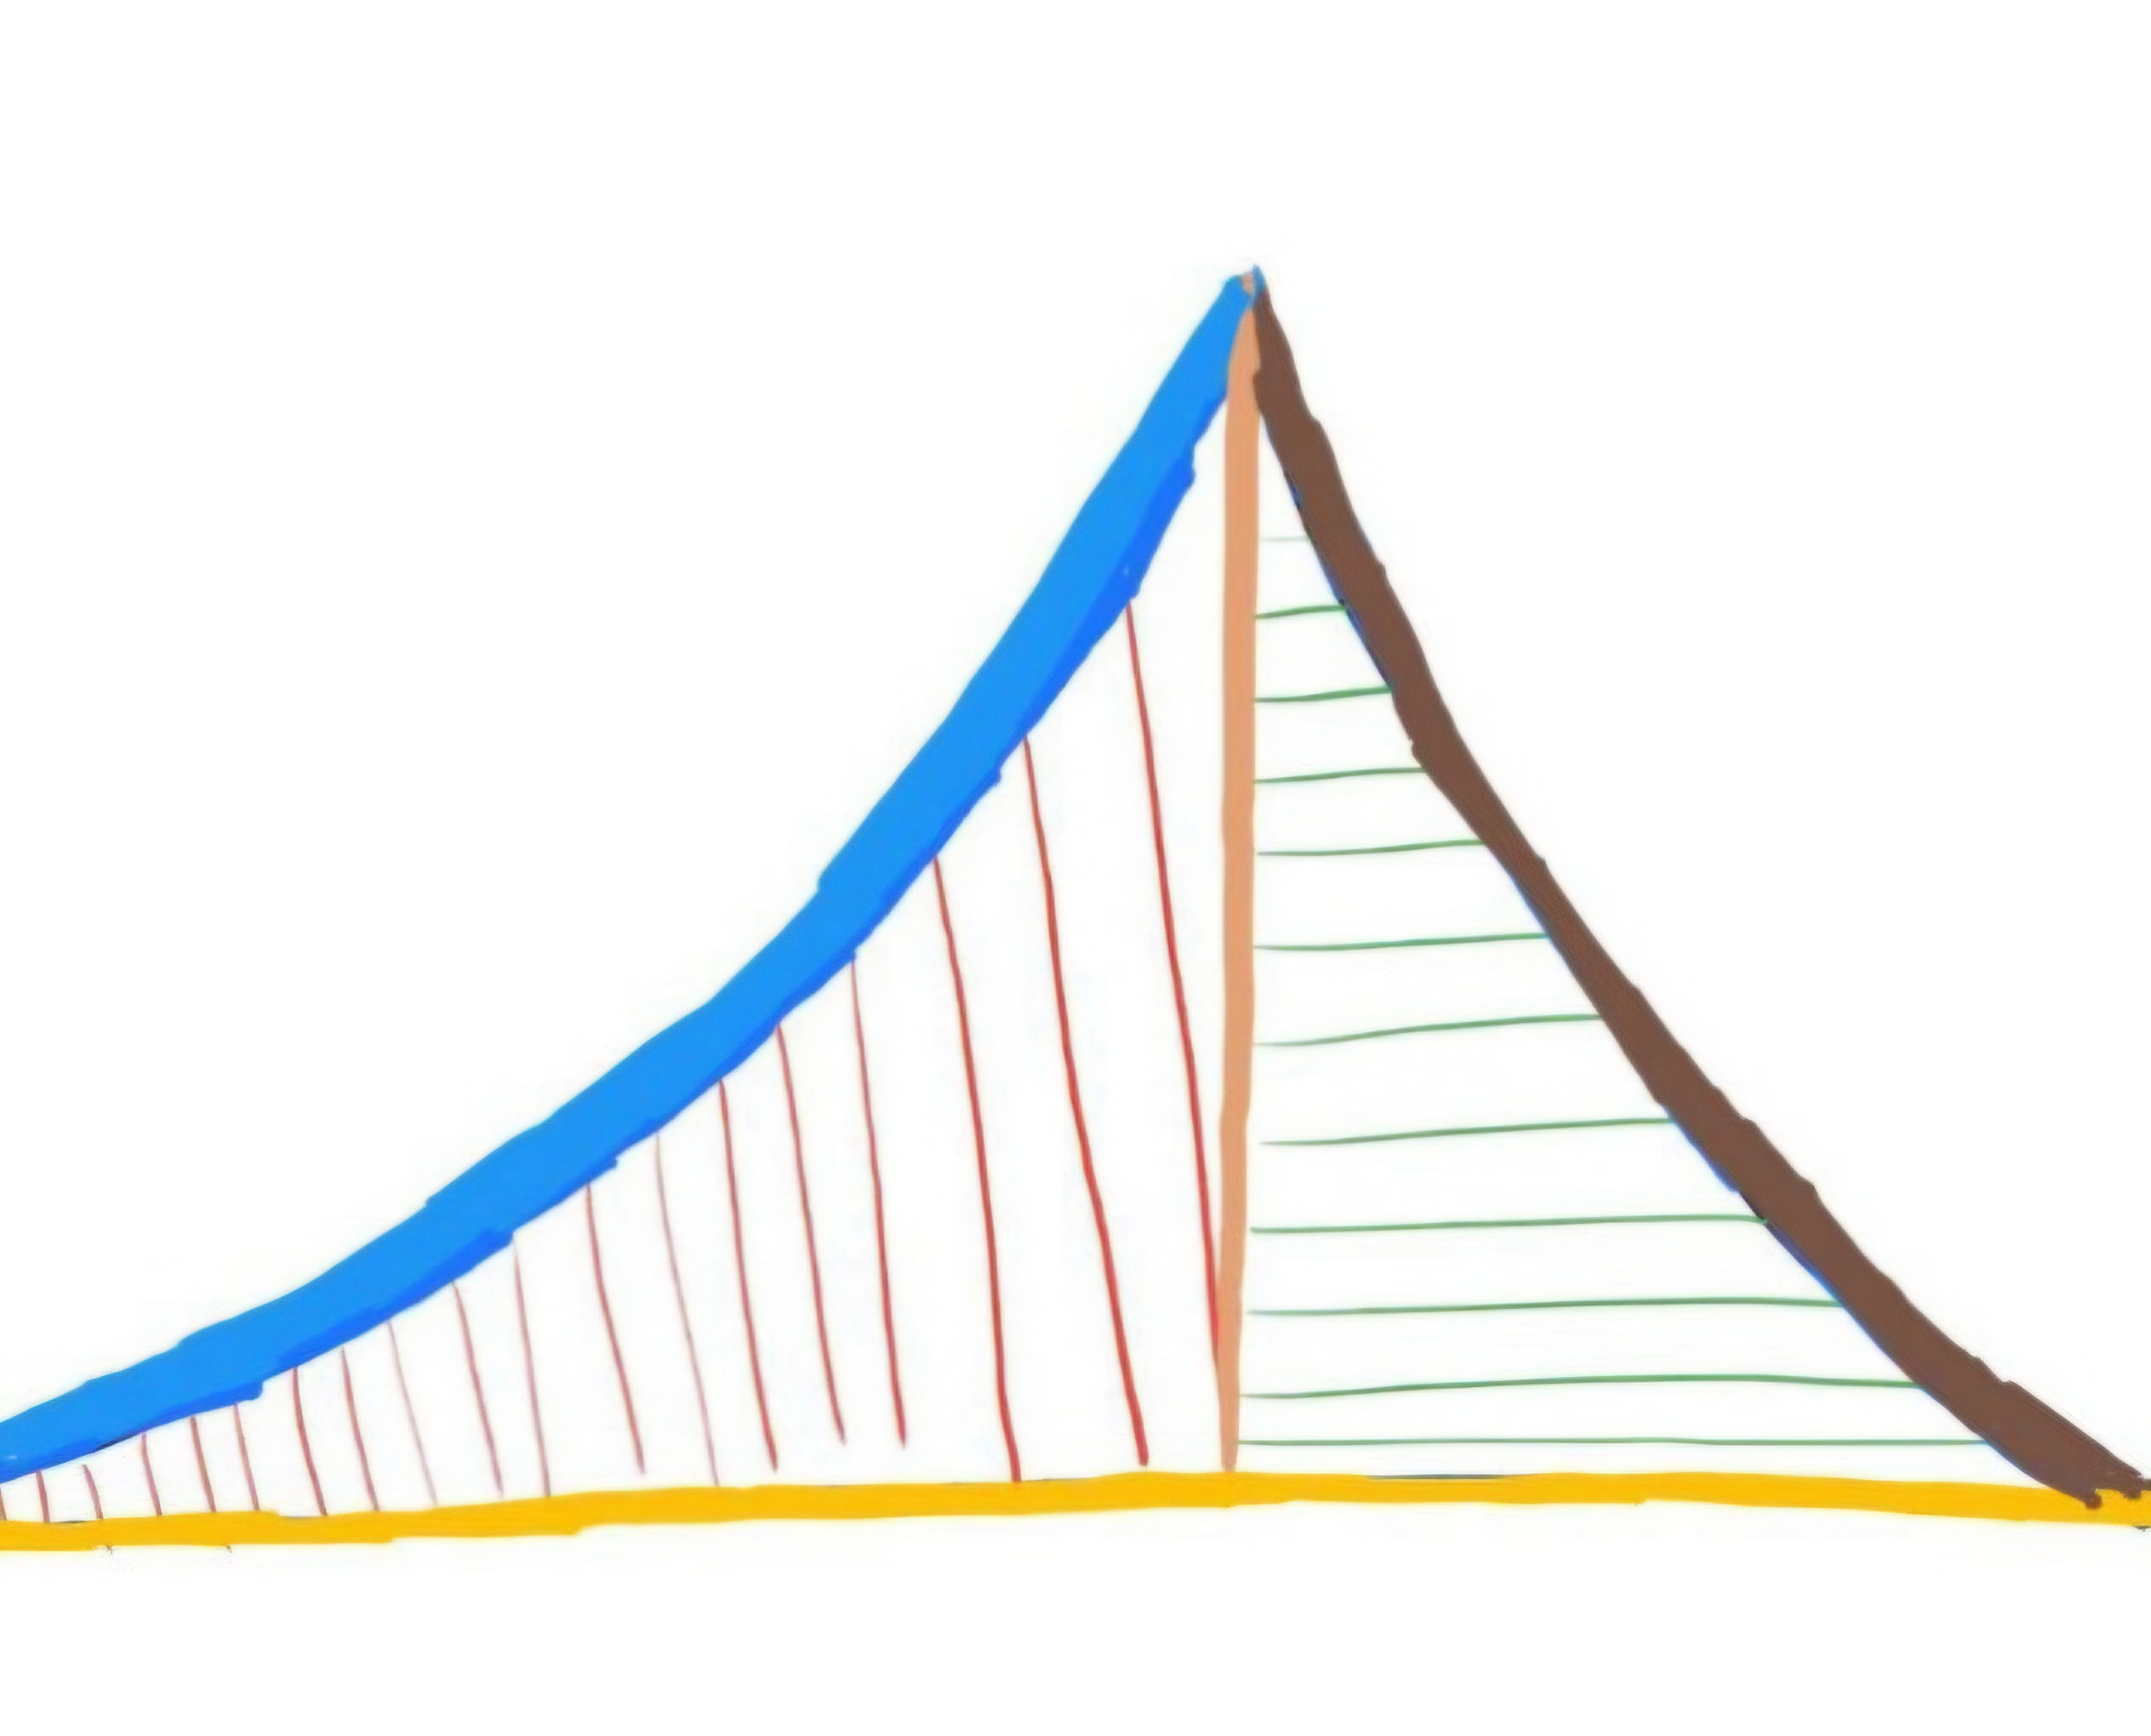
\includegraphics[width=0.2\columnwidth]{10/figs/logo.jpg}\\
    {\huge G. V. V. Sharma}
\end{center}
}

\maketitle
\newpage

\section*{About this Book}
This document contains the questions and solutions from the CBSE 2018 Mathematics question papers. Section 1 covers the unique questions from the Class 10 question paper sets. Section 2 covers the Class 12 question paper, Series BVM/5, Code No. 65/5/2 (Set 2).

Questions are typed in their original wording, with the original options and diagrams wherever applicable.

Where the same question appears in multiple sets, it will be included only once, provided the wording, values, options, and diagrams are identical.

\newpage
\tableofcontents
\newpage
\onecolumn

\numberwithin{equation}{enumi}
\numberwithin{figure}{enumi}
\renewcommand{\thetable}{\theenumi}

\section{CBSE CLASS-10 MATH 2018}
\subsection{Formulae}
\begin{enumerate}[label=\thesubsection.\arabic*, ref=\thesubsection.\theenumi]

\item If $x = \alpha$ is a root of $p(x) = ax^2 + bx + c = 0$, then $p(\alpha) = 0$, i.e.,
\begin{align}
	\myvec{\alpha^2 & \alpha & 1}\myvec{a \\ b \\ c} = a\alpha^2 + b\alpha + c = 0
	\label{eq:EE26BTECH11225-root}
\end{align}

\item If $\alpha$ and $\beta$ are distinct zeroes of $p(x)$, then $\brak{x - \alpha}\brak{x - \beta}$ is a factor of $p(x)$.
\begin{align}
	p\brak{x} = \brak{x - \alpha}\brak{x - \beta}q\brak{x}
	\label{eq:EE26BTECH11225-factor}
\end{align}
\solution
Dividing $p\brak{x}$ by $\brak{x - \alpha}$,
\begin{align}
	p\brak{x} = \brak{x - \alpha}s\brak{x} + p\brak{\alpha}
	= \brak{x - \alpha}s\brak{x}
\end{align}
since $p\brak{\alpha} = 0$. Substituting $x = \beta$,
\begin{align}
	p\brak{\beta} = \brak{\beta - \alpha}s\brak{\beta} = 0
	\implies s\brak{\beta} = 0
\end{align}
as $\beta \neq \alpha$. Repeating the division for $s\brak{x}$ with the zero $\beta$ gives
$s\brak{x} = \brak{x - \beta}q\brak{x}$, yielding \eqref{eq:EE26BTECH11225-factor}.

\item Roots of a quadratic equation $ax^2 + bx + c = 0$ $\brak{a \neq 0}$ and nature of roots, with discriminant $D = b^2 - 4ac$:
\begin{align}
	x &= \frac{-b \pm \sqrt{D}}{2a}
	\label{eq:EE26BTECH11225-quadratic}
	\\
	\begin{cases}
		D > 0 & \implies \text{two distinct real roots} \\
		D = 0 & \implies \text{two equal real roots} \\
		D < 0 & \implies \text{no real roots}
	\end{cases}
	\nonumber
\end{align}
\solution
Dividing by $a$ and completing the square,
\begin{align}
	x^2 + \frac{b}{a}x + \frac{c}{a} = 0
	\implies \brak{x + \frac{b}{2a}}^2 = \frac{b^2 - 4ac}{4a^2}
\end{align}
Taking the square root on both sides yields \eqref{eq:EE26BTECH11225-quadratic}. The roots are real only if $D \geq 0$. Further, for roots $\alpha, \beta$,
\begin{align}
	\alpha + \beta = -\frac{b}{a}, \quad \alpha\beta = \frac{c}{a}
\end{align}
which also follows from the fact that $\alpha, \beta$ are the eigenvalues of the companion matrix
\begin{align}
	\vec{C} = \myvec{0 & 1 \\ -\frac{c}{a} & -\frac{b}{a}},
	\quad
	\mydet{\vec{C} - \lambda\vec{I}} = \lambda^2 + \frac{b}{a}\lambda + \frac{c}{a}
\end{align}
with $\sum \lambda_i = \text{Tr}\brak{\vec{C}}$ and $\prod \lambda_i = \mydet{\vec{C}}$.

\item The $n^{\text{th}}$ term $a_n$ of an Arithmetic Progression (A.P.) with first term $a$ and common difference $d$:
\begin{align}
	a_n = a + \brak{n - 1}d
	\label{eq:EE26BTECH11225-ap-nth}
\end{align}
\solution
By definition $a_{k+1} - a_k = d$. Summing for $k = 1, 2, \ldots, n-1$ (telescoping),
\begin{align}
	\sum_{k=1}^{n-1}\brak{a_{k+1} - a_k} = a_n - a_1 = \brak{n - 1}d
\end{align}
and $a_1 = a$, yielding \eqref{eq:EE26BTECH11225-ap-nth}.

\item Sum of the first $n$ terms $S_n$ of an A.P.:
\begin{align}
	S_n = \frac{n}{2}\sbrak{2a + \brak{n - 1}d} = \frac{n}{2}\brak{a + l}
	\label{eq:EE26BTECH11225-ap-sum}
\end{align}
where $l = a_n$ is the last term.
\\
\solution
Writing the sum forwards and backwards,
\begin{align}
	S_n &= a_1 + a_2 + \cdots + a_n
	\\
	S_n &= a_n + a_{n-1} + \cdots + a_1
\end{align}
From \eqref{eq:EE26BTECH11225-ap-nth}, each pair satisfies
$a_k + a_{n+1-k} = 2a + \brak{n-1}d = a + l$. Adding the two equations,
\begin{align}
	2S_n = n\brak{a + l} = n\sbrak{2a + \brak{n - 1}d}
\end{align}
yielding \eqref{eq:EE26BTECH11225-ap-sum}.

\item Four consecutive terms in an A.P. with common difference $2d$:
\begin{align}
	\myvec{a - 3d \\ a - d \\ a + d \\ a + 3d}
	= a\vec{1} + d\myvec{-3 \\ -1 \\ 1 \\ 3}
	\label{eq:EE26BTECH11225-ap-four}
\end{align}
where $\vec{1}$ is the all-ones vector.
\\
\solution
The difference between any two consecutive entries is
\begin{align}
	\brak{a - d} - \brak{a - 3d} = \brak{a + d} - \brak{a - d} = \brak{a + 3d} - \brak{a + d} = 2d
\end{align}
and the mean of the four terms is $a$, which is why this choice simplifies the equations.

\item Distance between the points $\vec{P} = \myvec{x_1 \\ y_1}$ and $\vec{Q} = \myvec{x_2 \\ y_2}$:
\begin{align}
	d = \norm{\vec{Q} - \vec{P}}
	= \sqrt{\brak{\vec{Q} - \vec{P}}^{\top}\brak{\vec{Q} - \vec{P}}}
	= \sqrt{\brak{x_2 - x_1}^2 + \brak{y_2 - y_1}^2}
	\label{eq:EE26BTECH11225-distance}
\end{align}
\solution
The direction vector from $\vec{P}$ to $\vec{Q}$ is
\begin{align}
	\vec{Q} - \vec{P} = \myvec{x_2 - x_1 \\ y_2 - y_1}
\end{align}
and its length is the norm, obtained from the Pythagoras theorem, yielding \eqref{eq:EE26BTECH11225-distance}.

\item Section formula: the point $\vec{R}$ dividing the line joining $\vec{P}$ and $\vec{Q}$ internally in the ratio $k : 1$ is
\begin{align}
	\vec{R} = \frac{k\vec{Q} + \vec{P}}{k + 1}
	\iff
	\myvec{x \\ y} = \frac{1}{k + 1}\myvec{k x_2 + x_1 \\ k y_2 + y_1}
	\label{eq:EE26BTECH11225-section}
\end{align}
\solution
Since $\vec{R}$ lies on the line segment $PQ$ with $PR : RQ = k : 1$,
\begin{align}
	\vec{R} - \vec{P} &= k\brak{\vec{Q} - \vec{R}}
	\\
	\implies \brak{k + 1}\vec{R} &= k\vec{Q} + \vec{P}
\end{align}
yielding \eqref{eq:EE26BTECH11225-section}. For $k = 1$, $\vec{R}$ is the midpoint of $PQ$.

\item The area of a triangle with vertices $\vec{A} = \myvec{x_1 \\ y_1}$, $\vec{B} = \myvec{x_2 \\ y_2}$ and $\vec{C} = \myvec{x_3 \\ y_3}$ is
\begin{align}
	\text{Area}\brak{\Delta ABC}
	&= \frac{1}{2}\abs{\det\myvec{\vec{B} - \vec{A} & \vec{C} - \vec{A}}}
	\nonumber
	\\
	&= \frac{1}{2}\abs{x_1\brak{y_2 - y_3} + x_2\brak{y_3 - y_1} + x_3\brak{y_1 - y_2}}
	\label{eq:EE26BTECH11225-area-triangle}
\end{align}
The area of the quadrilateral $ABCD$, whose diagonal $AC$ lies inside it, is
\begin{align}
	\text{Area}\brak{ABCD} = \text{Area}\brak{\Delta ABC} + \text{Area}\brak{\Delta ADC}
	\label{eq:EE26BTECH11225-area-quad}
\end{align}
\solution
Let $\vec{a} = \vec{B} - \vec{A}$, $\vec{b} = \vec{C} - \vec{A}$ and let $\theta$ be the angle at $A$. Then
\begin{align}
	\text{Area}\brak{\Delta ABC} = \frac{1}{2}\norm{\vec{a}}\norm{\vec{b}}\sin\theta
\end{align}
Choosing $\vec{a} = \norm{\vec{a}}\myvec{\cos\phi \\ \sin\phi}$ and $\vec{b} = \norm{\vec{b}}\myvec{\cos\brak{\phi + \theta} \\ \sin\brak{\phi + \theta}}$,
\begin{align}
	\det\myvec{\vec{a} & \vec{b}}
	&= \norm{\vec{a}}\norm{\vec{b}}\sbrak{\cos\phi\sin\brak{\phi + \theta} - \sin\phi\cos\brak{\phi + \theta}}
	\\
	&= \norm{\vec{a}}\norm{\vec{b}}\sin\theta
\end{align}
Expanding the determinant,
\begin{align}
	\mydet{x_2 - x_1 & x_3 - x_1 \\ y_2 - y_1 & y_3 - y_1}
	= x_1\brak{y_2 - y_3} + x_2\brak{y_3 - y_1} + x_3\brak{y_1 - y_2}
\end{align}
yielding \eqref{eq:EE26BTECH11225-area-triangle}. The modulus accounts for the orientation of the vertices. The diagonal $AC$ splits $ABCD$ into $\Delta ABC$ and $\Delta ADC$, resulting in \eqref{eq:EE26BTECH11225-area-quad}.

\item Area Ratio Theorem for similar triangles $\Delta ABC \sim \Delta PQR$:
\begin{align}
	\frac{\text{ar}\brak{\Delta ABC}}{\text{ar}\brak{\Delta PQR}} = \brak{\frac{AB}{PQ}}^2
	\label{eq:EE26BTECH11225-area-ratio}
\end{align}
\solution
Similarity with scale factor $s = \frac{PQ}{AB}$ means there exist an orthogonal matrix $\vec{M}$, i.e., $\vec{M}^{\top}\vec{M} = \vec{I}$, with $\mydet{\vec{M}} = \pm 1$, and a vector $\vec{t}$ such that
\begin{align}
	\vec{P} = s\vec{M}\vec{A} + \vec{t}, \quad
	\vec{Q} = s\vec{M}\vec{B} + \vec{t}, \quad
	\vec{R} = s\vec{M}\vec{C} + \vec{t}
\end{align}
Then $\vec{Q} - \vec{P} = s\vec{M}\brak{\vec{B} - \vec{A}}$ and $\vec{R} - \vec{P} = s\vec{M}\brak{\vec{C} - \vec{A}}$. Using \eqref{eq:EE26BTECH11225-area-triangle} and $\mydet{\vec{X}\vec{Y}} = \mydet{\vec{X}}\mydet{\vec{Y}}$,
\begin{align}
	\text{ar}\brak{\Delta PQR}
	&= \frac{1}{2}\abs{\det\brak{s\vec{M}\myvec{\vec{B} - \vec{A} & \vec{C} - \vec{A}}}}
	\\
	&= \frac{s^2}{2}\abs{\det\vec{M}}\abs{\det\myvec{\vec{B} - \vec{A} & \vec{C} - \vec{A}}}
	= s^2\,\text{ar}\brak{\Delta ABC}
\end{align}
since $\mydet{s\vec{X}} = s^2\mydet{\vec{X}}$ for a $2 \times 2$ matrix. Hence
\begin{align}
	\frac{\text{ar}\brak{\Delta ABC}}{\text{ar}\brak{\Delta PQR}} = \frac{1}{s^2} = \brak{\frac{AB}{PQ}}^2
\end{align}

\item Tangent properties of a circle with centre $\vec{O}$ and radius $r$:
\begin{center}
	\begin{tikzpicture}[scale=0.8]
        \draw[thick] (0,0) circle (1.5cm);
        \coordinate (O) at (0,0);
        \coordinate (P) at (4,0);
        \coordinate (A) at (0.56, 1.39);
        \coordinate (B) at (0.56, -1.39);
        
        \draw[dashed] (O) -- (A);
        \draw[dashed] (O) -- (B);
        \draw[dashed] (O) -- (P);
        \draw[thick] (P) -- (A);
        \draw[thick] (P) -- (B);
        
        \filldraw (O) circle (1.5pt) node[left] {$O$};
        \filldraw (P) circle (1.5pt) node[right] {$P$};
        \filldraw (A) circle (1.5pt) node[above] {$A$};
        \filldraw (B) circle (1.5pt) node[below] {$B$};
        
        % Right angle symbol at A
        \draw (0.42,1.25) -- (0.55,1.12) -- (0.69,1.26);
    \end{tikzpicture}

\end{center}
Radius is perpendicular to the tangent at the point of contact:
\begin{align}
	\angle OAP = 90^\circ
	\iff \brak{\vec{O} - \vec{A}}^{\top}\brak{\vec{P} - \vec{A}} = 0
	\label{eq:EE26BTECH11225-tangent-perp}
\end{align}
Tangents drawn to a circle from an external point $P$ are equal in length:
\begin{align}
	PA = PB
	\label{eq:EE26BTECH11225-tangent-equal}
\end{align}
\solution
The tangent at $\vec{A}$ is the line $\vec{x} = \vec{A} + \lambda\vec{m}$. Its points of intersection with the circle $\norm{\vec{x} - \vec{O}}^2 = r^2$ satisfy
\begin{align}
	\norm{\vec{A} - \vec{O} + \lambda\vec{m}}^2 = r^2
	\implies \norm{\vec{m}}^2\lambda^2 + 2\lambda\,\vec{m}^{\top}\brak{\vec{A} - \vec{O}} = 0
\end{align}
using $\norm{\vec{A} - \vec{O}}^2 = r^2$. The roots are $\lambda = 0$ and $\lambda = -\frac{2\vec{m}^{\top}\brak{\vec{A} - \vec{O}}}{\norm{\vec{m}}^2}$. A tangent touches the circle at only one point, so both roots must be zero, yielding
$\vec{m}^{\top}\brak{\vec{A} - \vec{O}} = 0$, which is \eqref{eq:EE26BTECH11225-tangent-perp} since $\vec{P} - \vec{A}$ is along $\vec{m}$.
\\
Now,
\begin{align}
	\norm{\vec{P} - \vec{O}}^2
	&= \norm{\brak{\vec{P} - \vec{A}} + \brak{\vec{A} - \vec{O}}}^2
	\\
	&= \norm{\vec{P} - \vec{A}}^2 + 2\brak{\vec{P} - \vec{A}}^{\top}\brak{\vec{A} - \vec{O}} + r^2
	\\
	\implies PA^2 &= \norm{\vec{P} - \vec{O}}^2 - r^2
\end{align}
by \eqref{eq:EE26BTECH11225-tangent-perp}. The same steps give $PB^2 = \norm{\vec{P} - \vec{O}}^2 - r^2$, yielding \eqref{eq:EE26BTECH11225-tangent-equal}.

\item Pythagoras Theorem in a right-angled triangle $ABC$ with $\angle B = 90^\circ$:
\begin{align}
	\text{Hypotenuse}^2 = \text{Base}^2 + \text{Height}^2
	\iff
	\norm{\vec{A} - \vec{C}}^2 = \norm{\vec{A} - \vec{B}}^2 + \norm{\vec{C} - \vec{B}}^2
	\label{eq:EE26BTECH11225-pythagoras}
\end{align}
\solution
The right angle at $B$ means
\begin{align}
	\brak{\vec{A} - \vec{B}}^{\top}\brak{\vec{C} - \vec{B}} = 0
\end{align}
Writing $\vec{A} - \vec{C} = \brak{\vec{A} - \vec{B}} - \brak{\vec{C} - \vec{B}}$,
\begin{align}
	\norm{\vec{A} - \vec{C}}^2
	= \norm{\vec{A} - \vec{B}}^2 + \norm{\vec{C} - \vec{B}}^2 - 2\brak{\vec{A} - \vec{B}}^{\top}\brak{\vec{C} - \vec{B}}
\end{align}
yielding \eqref{eq:EE26BTECH11225-pythagoras}.

\item Fundamental trigonometric identities and standard ratios:
\begin{align}
	\sin^2 A + \cos^2 A &= 1
	\label{eq:EE26BTECH11225-trig-1}
	\\
	\sec^2 A - \tan^2 A &= 1
	\label{eq:EE26BTECH11225-trig-2}
	\\
	\csc^2 A - \cot^2 A &= 1
	\label{eq:EE26BTECH11225-trig-3}
\end{align}
For a vector $\vec{x} = \myvec{\text{Adjacent} \\ \text{Opposite}}$ making an angle $\theta$ with $\vec{e}_1$,
\begin{align}
	\begin{split}
		\sin\theta &= \frac{\text{Opposite}}{\text{Hypotenuse}} = \frac{\vec{e}_2^{\top}\vec{x}}{\norm{\vec{x}}}
		\\
		\cos\theta &= \frac{\text{Adjacent}}{\text{Hypotenuse}} = \frac{\vec{e}_1^{\top}\vec{x}}{\norm{\vec{x}}}
		\\
		\tan\theta &= \frac{\text{Opposite}}{\text{Adjacent}} = \frac{\vec{e}_2^{\top}\vec{x}}{\vec{e}_1^{\top}\vec{x}}
	\end{split}
	\label{eq:EE26BTECH11225-trig-ratios}
\end{align}
\solution
The point $\vec{r}\brak{A} = \myvec{\cos A \\ \sin A}$ lies on the unit circle, so
\begin{align}
	\norm{\vec{r}\brak{A}}^2 = \vec{r}\brak{A}^{\top}\vec{r}\brak{A} = \cos^2 A + \sin^2 A = 1
\end{align}
yielding \eqref{eq:EE26BTECH11225-trig-1}. Dividing by $\cos^2 A$ and $\sin^2 A$ respectively,
\begin{align}
	1 + \tan^2 A = \sec^2 A, \quad \cot^2 A + 1 = \csc^2 A
\end{align}
which are \eqref{eq:EE26BTECH11225-trig-2} and \eqref{eq:EE26BTECH11225-trig-3}.

\item Complementary angle identities:
\begin{align}
	\begin{split}
		\cos\brak{90^\circ - \theta} &= \sin\theta
		\\
		\tan\brak{90^\circ - \theta} &= \cot\theta
	\end{split}
	\label{eq:EE26BTECH11225-complementary}
\end{align}
\solution
Rotating the unit vector at angle $-\theta$ by $90^\circ$ using the rotation matrix,
\begin{align}
	\myvec{\cos\brak{90^\circ - \theta} \\ \sin\brak{90^\circ - \theta}}
	= \myvec{0 & -1 \\ 1 & 0}\myvec{\cos\theta \\ -\sin\theta}
	= \myvec{\sin\theta \\ \cos\theta}
\end{align}
yielding the first identity. Dividing the second row by the first,
\begin{align}
	\tan\brak{90^\circ - \theta} = \frac{\cos\theta}{\sin\theta} = \cot\theta
\end{align}

\item Area of a circular sector with central angle $\theta$:
\begin{align}
	\text{Area} = \frac{\theta}{360^\circ} \times \pi r^2
	\label{eq:EE26BTECH11225-sector}
\end{align}
\item Curved surface areas of a cylinder and a hemisphere of radius $r$:
\begin{align}
	\text{CSA of cylinder} &= 2\pi rh
	\label{eq:EE26BTECH11225-csa-cyl}
	\\
	\text{CSA of hemisphere} &= 2\pi r^2
	\label{eq:EE26BTECH11225-csa-hemi}
\end{align}
\item Volume, slant height, and curved surface area of a cone of base radius $r$ and height $h$:
\begin{align}
	V &= \frac{1}{3}\pi r^2 h
	\label{eq:EE26BTECH11225-cone-vol}
	\\
	l = \norm{\myvec{r \\ h}} &= \sqrt{r^2 + h^2}, \quad \text{CSA} = \pi r l
	\label{eq:EE26BTECH11225-cone-csa}
\end{align}
\solution
By similar triangles, the cross-section at height $z$ from the apex has radius $\frac{rz}{h}$. Integrating the areas of the circular cross-sections,
\begin{align}
	V = \int_{0}^{h}\pi\brak{\frac{rz}{h}}^2 dz = \frac{\pi r^2}{h^2}\sbrak{\frac{z^3}{3}}_{0}^{h} = \frac{1}{3}\pi r^2 h
\end{align}
The slant height is the length of the vector $\myvec{r \\ h}$. Cutting the cone along a slant line and unrolling it gives a sector of radius $l$ and arc length $2\pi r$, so the angle is $\theta_r = \frac{2\pi r}{l}$. From \eqref{eq:EE26BTECH11225-sector} in radians,
\begin{align}
	\text{CSA} = \frac{1}{2}l^2\theta_r = \pi r l
\end{align}

\item Slant height and surface area of an open frustum with radii $R > r$ and height $h$:
\begin{align}
	l = \norm{\myvec{R - r \\ h}} &= \sqrt{h^2 + \brak{R - r}^2}
	\label{eq:EE26BTECH11225-frustum-l}
	\\
	\text{Area} &= \pi\brak{R + r}l + \pi r^2
	\label{eq:EE26BTECH11225-frustum-area}
\end{align}
\solution
The slant height is the length of the vector $\myvec{R - r \\ h}$. Let $L$ be the slant height of the full cone of base radius $R$. The removed cone has radius $r$ and slant height $L - l$. By similar triangles,
\begin{align}
	\frac{r}{R} = \frac{L - l}{L}
	\implies L = \frac{lR}{R - r}
\end{align}
Subtracting the curved surface areas using \eqref{eq:EE26BTECH11225-cone-csa},
\begin{align}
	\text{CSA} = \pi RL - \pi r\brak{L - l}
	= \pi\sbrak{\brak{R - r}L + rl}
	= \pi\brak{R + r}l
\end{align}
Adding the circular base of radius $r$ yields \eqref{eq:EE26BTECH11225-frustum-area}.

\item Direct method for the mean and the grouped median formula, for class marks $x_i$ and frequencies $f_i$:
\begin{align}
	\bar{x} &= \frac{\sum f_i x_i}{\sum f_i} = \frac{\vec{f}^{\top}\vec{x}}{\vec{f}^{\top}\vec{1}}
	\label{eq:EE26BTECH11225-mean}
	\\
	\text{Median} &= l + \brak{\frac{\frac{N}{2} - cf}{f}} \times h
	\label{eq:EE26BTECH11225-median}
\end{align}
where $N = \sum f_i$, $l$ is the lower limit, $h$ the width and $f$ the frequency of the median class, and $cf$ the cumulative frequency of the class preceding it.
\\
\solution
The mean $m$ minimizes the weighted squared error
\begin{align}
	J\brak{m} = \sum f_i\brak{x_i - m}^2
	\implies \frac{dJ}{dm} = -2\sum f_i\brak{x_i - m} = 0
	\implies m = \frac{\sum f_i x_i}{\sum f_i}
\end{align}
yielding \eqref{eq:EE26BTECH11225-mean}. For the median, assuming the frequency is uniformly spread over the median class, the cumulative frequency is linear in that class,
\begin{align}
	F\brak{x} = cf + \frac{f}{h}\brak{x - l}
\end{align}
The median is the value where $F\brak{x} = \frac{N}{2}$,
\begin{align}
	\frac{N}{2} = cf + \frac{f}{h}\brak{x - l}
	\implies x = l + \brak{\frac{\frac{N}{2} - cf}{f}} \times h
\end{align}
yielding \eqref{eq:EE26BTECH11225-median}.

\item The unit step function, and an A.P. with first term $a$ and common difference $d$ written as a sequence:
\begin{align}
u(n) &= \begin{cases} 1, & n \ge 0 \\ 0, & n < 0 \end{cases} \label{eq:EE26BTECH11225-unit-step} \\
x(n) &= \brak{a + (n-1)d}\,u(n-1) \label{eq:EE26BTECH11225-ap-step}
\end{align}
Thus $x(n) = 0$ for $n < 1$ and $x(n) = a_n$ for $n \ge 1$.
\item Newton--Raphson iteration to find a root of $f(x) = 0$ from a starting value $x_0$:
\begin{align}
x_{n+1} = x_n - \frac{f(x_n)}{f'(x_n)}, \quad f'(x_n) \ne 0 \label{eq:EE26BTECH11225-newton}
\end{align}
\solution The tangent to $y = f(x)$ at $x = x_n$ is $y = f(x_n) + f'(x_n)(x - x_n)$. It meets the $x$-axis where $y = 0$, which gives $x_{n+1}$ above.
\item Probability mass function (PMF) of a discrete random variable $X$, and of a pair $(X,Y)$:
\begin{align}
p_X(k) &= \Pr\brak{X = k}, \quad \sum_k p_X(k) = 1, \quad \Pr\brak{X \in E} = \sum_{k \in E} p_X(k) \label{eq:EE26BTECH11225-pmf} \\
p_{XY}(i,j) &= p_X(i)\,p_Y(j) \quad \text{when $X$ and $Y$ are independent} \label{eq:EE26BTECH11225-pmf-joint}
\end{align}
\end{enumerate}

\subsection{Problems}
\graphicspath{{10/}}
\begin{enumerate}[label=\thesubsection.\arabic*, ref=\thesubsection.\theenumi]
    \item If $x = 3$ is one root of the quadratic equation $x^2 - 2kx - 6 = 0$, then find the value of $k$.

\solution Since $x = 3$ is a root of the given quadratic equation, from \eqref{eq:EE26BTECH11225-root}, substituting $x = 3$ into $x^2 - 2kx - 6 = 0$:
\begin{align}
    (3)^2 - 2k(3) - 6 &= 0 \\
    &\implies 9 - 6k - 6 = 0 \\
    &\implies 3 - 6k = 0 \\
    &\implies 6k = 3 
\end{align}
Thus, the value of $k$ is $\frac{1}{2}$.
    \item What is the HCF of smallest prime number and the smallest composite number?

\solution 
\begin{align}
    \text{Smallest prime number} &= 2 \\
    \text{Smallest composite number} &= 4
\end{align}
Expressing both as prime factors:
\begin{align}
    2 &= 2^1 \\
    4 &= 2^2 \\
    &\implies \text{HCF}(2, 4) = 2^1 = 2
\end{align}
    \item Find the distance of a point $P(x, y)$ from the origin.

\solution From \eqref{eq:EE26BTECH11225-distance}, the distance of $P(x, y)$ from $O(0, 0)$ is:
\begin{align}
    d &= \sqrt{(x - 0)^2 + (y - 0)^2} \\
    &= \sqrt{x^2 + y^2}
\end{align}
    \item In an AP, if the common difference $(d) = -4$, and the seventh term $(a_7)$ is 4, then find the first term.

\solution
The A.P. is the sequence $x(n)$ with first term $a$ and common difference $d = -4$. From \eqref{eq:EE26BTECH11225-ap-step},
\begin{align}
x(n) = \brak{a + (n-1)d}\,u(n-1) = \brak{a - 4(n-1)}\,u(n-1)
\end{align}
\par\noindent\hfill\mbox{\textit{(\ref{eq:EE26BTECH11225-ap-step})}}\par
Since $u(6) = 1$, the seventh term is $x(7) = a - 24$. Equating it to the given value,
\begin{align}
a - 24 = 4 \implies a = 28
\end{align}
The first term is therefore $\boxed{28}$. The C program prints the sequence, which the unit step switches on at $n = 1$, and the Python program plots it in \figref{fig:ap_q4}.
\begin{lstlisting}[frame=single, basicstyle=\rmfamily, escapeinside={(*@}{@*)}]
(*@\makebox[\dimexpr\linewidth-2\fboxsep-2\fboxrule\relax][c]{codes/1.2.4.c}@*)
\end{lstlisting}
\begin{lstlisting}[frame=single, basicstyle=\rmfamily, escapeinside={(*@}{@*)}]
(*@\makebox[\dimexpr\linewidth-2\fboxsep-2\fboxrule\relax][c]{codes/1.2.4.py}@*)
\end{lstlisting}
\begin{figure}[H]
    \centering
    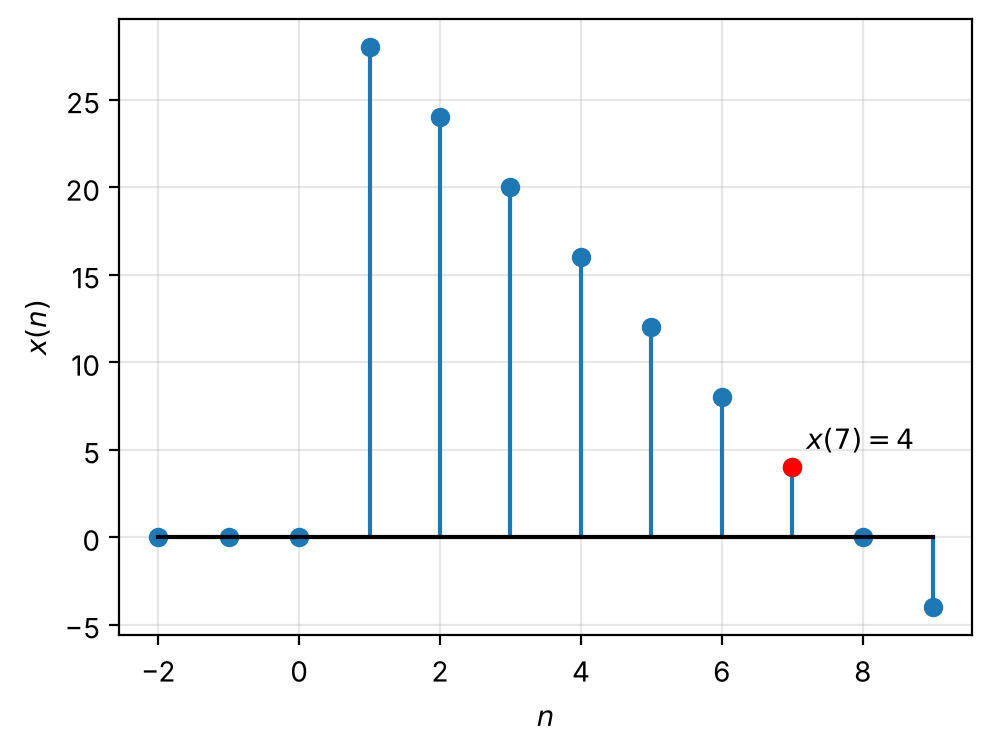
\includegraphics[width=0.65\linewidth]{figs/1.2.4.png}
    \caption{The A.P. as the sequence $x(n) = (a + (n-1)d)\,u(n-1)$}
    \label{fig:ap_q4}
\end{figure}

	\item What is the value of $(\cos^2 67^\circ - \sin^2 23^\circ)$?

\solution From \eqref{eq:EE26BTECH11225-complementary}, $\cos(90^\circ - \theta) = \sin \theta$:
\begin{align}
    \cos 67^\circ &= \cos(90^\circ - 23^\circ) \\
    &\implies \cos 67^\circ = \sin 23^\circ \\
    &\implies \cos^2 67^\circ - \sin^2 23^\circ = \sin^2 23^\circ - \sin^2 23^\circ = 0
\end{align}
    \item Given $\Delta ABC \sim \Delta PQR$, if $\frac{AB}{PQ} = \frac{1}{3}$, then find $\frac{\text{ar}(\Delta ABC)}{\text{ar}(\Delta PQR)}$.

\solution From \eqref{eq:EE26BTECH11225-area-ratio} (area ratio theorem for similar triangles):
\begin{align}
    \frac{\text{ar}(\Delta ABC)}{\text{ar}(\Delta PQR)} &= \left(\frac{AB}{PQ}\right)^2 \\
    &\implies \frac{\text{ar}(\Delta ABC)}{\text{ar}(\Delta PQR)} = \left(\frac{1}{3}\right)^2 = \frac{1}{9}
\end{align}
    \item Given that $\sqrt{2}$ is irrational, prove that $(5+3\sqrt{2})$ is an irrational number.

\solution Assume $(5+3\sqrt{2})$ is rational, so $5+3\sqrt{2} = \frac{a}{b}$ where $a, b \in \mathbb{Z}, b \neq 0$:
\begin{align}
    3\sqrt{2} &= \frac{a}{b} - 5 \\
    &\implies \sqrt{2} = \frac{a - 5b}{3b}
\end{align}
Since $a, b \in \mathbb{Z}$, the expression $\frac{a - 5b}{3b}$ is rational. This contradicts the given fact that $\sqrt{2}$ is irrational. Hence, $(5+3\sqrt{2})$ is irrational.

    \item In \figref{fig:rectangle_q8}, $ABCD$ is a rectangle. Find the values of $x$ and $y$.
    \begin{figure}[H]
\centering
\begin{tikzpicture}[scale=0.85]
    % Draw the rectangle box (width 6, height 3)
    \draw[line width=1.2pt] (0,0) -- (6,0) -- (6,3) -- (0,3) -- cycle;

    % Vertex labels (A, B, C, D)
    \node[below left] at (0,0) {\textbf{A}};
    \node[below right] at (6,0) {\textbf{B}};
    \node[above right] at (6,3) {\textbf{C}};
    \node[above left] at (0,3) {\textbf{D}};

    % Side measurement labels
    \node[below] at (3, 0) {$30\text{ cm}$};
    \node[right] at (6, 1.5) {$x - y$};
    \node[above] at (3, 3) {$x + y$};
    \node[left] at (0, 1.5) {$14\text{ cm}$};
\end{tikzpicture}

\caption{Rectangle $ABCD$}
\label{fig:rectangle_q8}
\end{figure} 

\solution Opposite sides of a rectangle are equal in length.
\begin{align}
    x + y &= 30 \label{eq:EE26BTECH11225-rect-1} \\
    x - y &= 14 \label{eq:EE26BTECH11225-rect-2}
\end{align}
Adding \eqref{eq:EE26BTECH11225-rect-1} and \eqref{eq:EE26BTECH11225-rect-2}:
\begin{align}
    (x + y) + (x - y) &= 30 + 14 \\
    &\implies 2x = 44 \\
    &\implies x = 22
\end{align}
Substituting $x = 22$ into \eqref{eq:EE26BTECH11225-rect-1}:
\begin{align}
    22 + y &= 30 \\
    &\implies y = 30 - 22 \\
    &\implies y = 8
\end{align}
Thus, $x = 22$ and $y = 8$.
    \item Find the sum of first 8 multiples of 3.

\solution The first 8 multiples of 3 form an A.P.: $3, 6, 9, \dots$ with first term $a = 3$, common difference $d = 3$, and $n = 8$. From \eqref{eq:EE26BTECH11225-ap-sum},
\begin{align}
    S_n &= \frac{n}{2}[2a + (n-1)d] \\
    &\implies S_8 = \frac{8}{2}[2(3) + (8-1)3] \\
    &\implies S_8 = 4[6 + 21] \\
    &\implies S_8 = 4(27) = 108
\end{align}
    \item Find the ratio in which $P(4, m)$ divides the line segment joining the points $A(2, 3)$ and $B(6, -3)$. Hence find $m$.

\solution Let $P(4, m)$ divide $AB$ in the ratio $k : 1$. From \eqref{eq:EE26BTECH11225-section}, for the $x$-coordinate:
\begin{align}
    x &= \frac{k(x_2) + 1(x_1)}{k + 1} \\
    &\implies 4 = \frac{k(6) + 1(2)}{k + 1} \\
    &\implies 4(k + 1) = 6k + 2 \\
    &\implies 4k + 4 = 6k + 2 \\
    &\implies 2k = 2 \implies k = 1
\end{align}
Thus, the ratio is $1 : 1$. Now from \eqref{eq:EE26BTECH11225-section}, for the $y$-coordinate:
\begin{align}
    m &= \frac{1(-3) + 1(3)}{1 + 1} \\
    &\implies m = \frac{0}{2} = 0
\end{align}The following code verifies the result and generates \figref{fig:section_q10}.
\begin{lstlisting}[frame=single, basicstyle=\rmfamily, escapeinside={(*@}{@*)}]
(*@\makebox[\dimexpr\linewidth-2\fboxsep-2\fboxrule\relax][c]{codes/1.2.10.py}@*)
\end{lstlisting}
\begin{figure}[H]
    \centering
    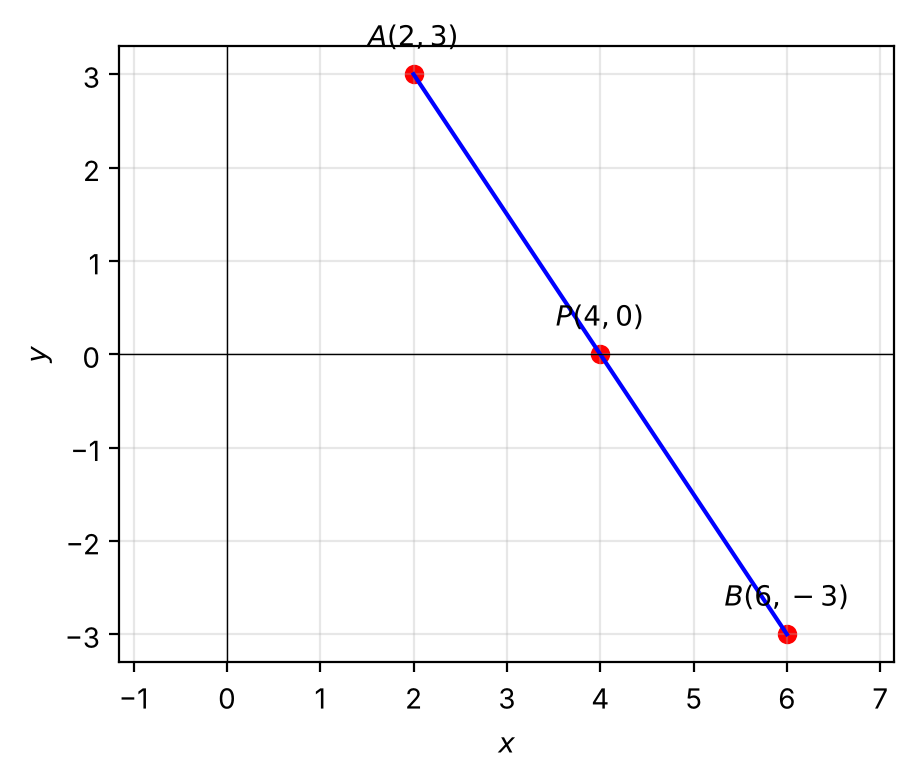
\includegraphics[width=0.60\linewidth]{figs/1.2.10.png}
    \caption{Point $P$ dividing $AB$}
    \label{fig:section_q10}
\end{figure}

    \item Two different dice are tossed together. Find the probability: \\[2pt]
(i) of getting a doublet. \\[2pt]
(ii) of getting a sum 10, of the numbers on the two dice.

\solution Let $X$ and $Y$ be the numbers on the two dice. They are independent and each is uniform on $\{1,\dots,6\}$, so from \eqref{eq:EE26BTECH11225-pmf-joint},
\begin{align}
    p_{XY}(i,j) = \frac{1}{6}\cdot\frac{1}{6} = \frac{1}{36}, \quad i,j \in \{1,\dots,6\}
\end{align}
(i) A doublet means $X = Y$. From \eqref{eq:EE26BTECH11225-pmf},
\begin{align}
    \Pr\brak{X = Y} = \sum_{i=1}^{6} p_{XY}(i,i) = 6 \cdot \frac{1}{36} = \frac{1}{6}
\end{align}
(ii) A sum of 10 means $(X,Y) \in \{(4,6),(5,5),(6,4)\}$:
\begin{align}
    \Pr\brak{X + Y = 10} = \sum_{i=4}^{6} p_{XY}(i,10-i) = 3 \cdot \frac{1}{36} = \frac{1}{12}
\end{align}
The following code builds the joint PMF of the two dice and verifies both probabilities.
\begin{lstlisting}[frame=single, basicstyle=\rmfamily, escapeinside={(*@}{@*)}]
(*@\makebox[\dimexpr\linewidth-2\fboxsep-2\fboxrule\relax][c]{codes/1.2.11.py}@*)
\end{lstlisting}

    \item An integer is chosen at random between 1 and 100. Find the probability that it is: \\[2pt]
(i) divisible by 8. \\[2pt]
(ii) not divisible by 8.

\solution Taking ``between $1$ and $100$'' to exclude both $1$ and $100$, the integer $X$ takes the values $2,3,\dots,99$, which are $98$ equally likely values. Its PMF is
\begin{align}
    p_X(k) = \frac{1}{98}, \quad k \in \{2,3,\dots,99\}
\end{align}
(i) The multiples of $8$ are $E = \{8,16,\dots,96\}$, which has $12$ values. From \eqref{eq:EE26BTECH11225-pmf},
\begin{align}
    \Pr\brak{8 \mid X} = \sum_{k \in E} p_X(k) = \frac{12}{98} = \frac{6}{49}
\end{align}
(ii) Since $\sum_k p_X(k) = 1$,
\begin{align}
    \Pr\brak{8 \nmid X} = 1 - \sum_{k \in E} p_X(k) = 1 - \frac{6}{49} = \frac{43}{49}
\end{align}
\item Find HCF and LCM of 404 and 96 and verify that $\text{HCF} \times \text{LCM} = \text{Product of the two given numbers}$.

\solution Expressing numbers as products of prime factors:
\begin{align}
    404 &= 2^2 \times 101 \\
    96 &= 2^5 \times 3 \\
    &\implies \text{HCF}(404, 96) = 2^2 = 4 \\
    &\implies \text{LCM}(404, 96) = 2^5 \times 3 \times 101 = 9696
\end{align}
Verification:
\begin{align}
    \text{LHS} &= \text{HCF} \times \text{LCM} = 4 \times 9696 = 38784 \\
    \text{RHS} &= 404 \times 96 = 38784 \\
    &\implies \text{LHS} = \text{RHS}
\end{align}
    \item Find all zeroes of the polynomial $(2x^4 - 9x^3 + 5x^2 + 3x - 1)$ if two of its zeroes are $(2+\sqrt{3})$ and $(2-\sqrt{3})$.

\solution Given zeroes $x = 2 \pm \sqrt{3}$, from \eqref{eq:EE26BTECH11225-factor}, $(x-\alpha)(x-\beta)$ is a factor of $p(x)$:
\begin{align}
    [x - (2 + \sqrt{3})][x - (2 - \sqrt{3})] &= (x - 2)^2 - 3 \\
    &= x^2 - 4x + 4 - 3 \\
    &\implies g(x) = x^2 - 4x + 1 \text{ is a factor}
\end{align}
Dividing $p(x) = 2x^4 - 9x^3 + 5x^2 + 3x - 1$ by $g(x) = x^2 - 4x + 1$:
\begin{align}
    2x^4 - 9x^3 + 5x^2 + 3x - 1 &= (x^2 - 4x + 1)(2x^2 - x - 1)
\end{align}
To find the remaining zeroes, set $2x^2 - x - 1 = 0$:
\begin{align}
    2x^2 - 2x + x - 1 &= 0 \\
    2x(x - 1) + 1(x - 1) &= 0 \\
    (2x + 1)(x - 1) &= 0 \\
    &\implies x = 1 \quad \text{or} \quad x = -\frac{1}{2}
\end{align}
Thus, all zeroes are $2+\sqrt{3}$, $2-\sqrt{3}$, $1$, and $-\frac{1}{2}$.The following code verifies the zeroes and plots $p(x)$ in \figref{fig:poly_q14}.
\begin{lstlisting}[frame=single, basicstyle=\rmfamily, escapeinside={(*@}{@*)}]
(*@\makebox[\dimexpr\linewidth-2\fboxsep-2\fboxrule\relax][c]{codes/1.2.14.py}@*)
\end{lstlisting}
\begin{figure}[H]
    \centering
    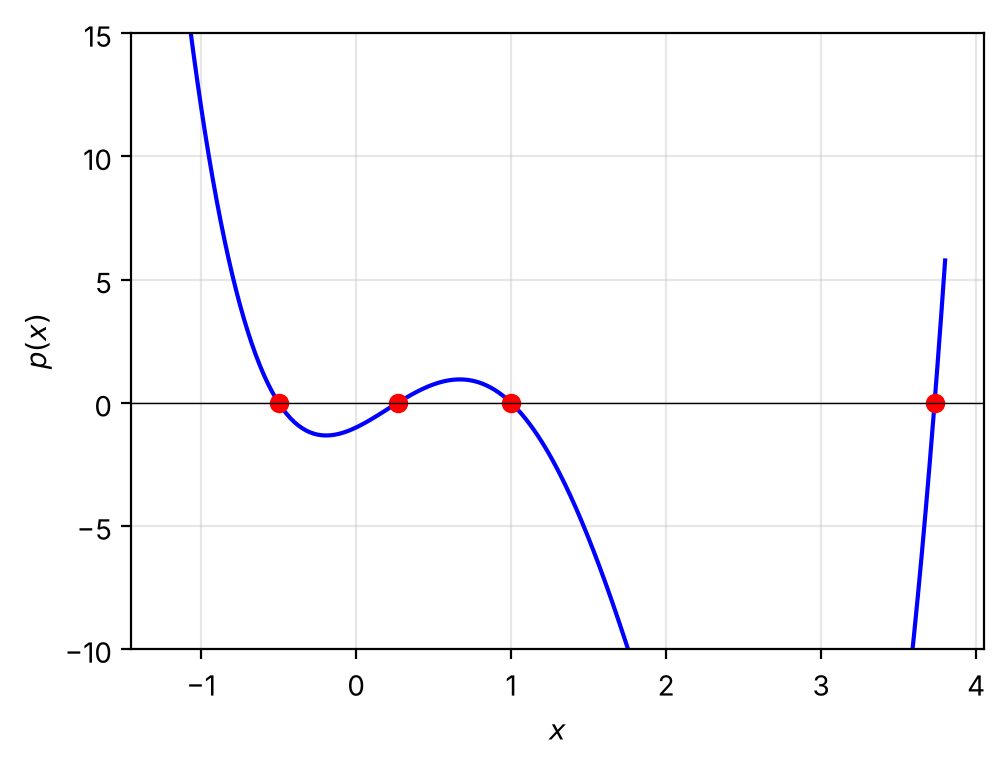
\includegraphics[width=0.70\linewidth]{figs/1.2.14.png}
    \caption{Plot of $p(x)=2x^4-9x^3+5x^2+3x-1$ with its zeroes}
    \label{fig:poly_q14}
\end{figure}

   \item 
    \begin{enumerate}[label=(\alph*), leftmargin=*, labelsep=0.5em]
        \item If $A(-2,1)$, $B(a,0)$, $C(4,b)$ and $D(1,2)$ are the vertices of a parallelogram $ABCD$, find the values of $a$ and $b$. Hence find the lengths of its sides.
        
        \begin{center}
            \textbf{OR}
        \end{center}
        
        \item If $A(-5,7)$, $B(-4,-5)$, $C(-1,-6)$ and $D(4,5)$ are the vertices of a quadrilateral, find the area of the quadrilateral $ABCD$.
    \end{enumerate} \vspace{2pt}
    \textbf{(a) Solution:} In a parallelogram, the diagonals bisect each other. Therefore, the midpoint of diagonal $AC$ is equal to the midpoint of diagonal $BD$.

From \eqref{eq:EE26BTECH11225-section} with $k=1$, the midpoint of $AC$ is:
\begin{align}
    M_{AC} &= \left( \frac{-2 + 4}{2}, \frac{1 + b}{2} \right) = \left( 1, \frac{1 + b}{2} \right)
\end{align}
Midpoint of $BD$:
\begin{align}
    M_{BD} &= \left( \frac{a + 1}{2}, \frac{0 + 2}{2} \right) = \left( \frac{a + 1}{2}, 1 \right)
\end{align}
Equating the $x$-coordinates and $y$-coordinates:
\begin{align}
    \frac{a + 1}{2} = 1 &\implies a + 1 = 2 \implies a = 1 \\
    \frac{1 + b}{2} = 1 &\implies 1 + b = 2 \implies b = 1
\end{align}
Thus, the vertices are $A(-2,1)$, $B(1,0)$, $C(4,1)$, and $D(1,2)$. \\[4pt]
Now, from \eqref{eq:EE26BTECH11225-distance}, the lengths of the sides are:
\begin{align}
    AB &= \sqrt{(1 - (-2))^2 + (0 - 1)^2} = \sqrt{3^2 + (-1)^2} = \sqrt{9 + 1} = \sqrt{10} \\
    BC &= \sqrt{(4 - 1)^2 + (1 - 0)^2} = \sqrt{3^2 + 1^2} = \sqrt{9 + 1} = \sqrt{10}
\end{align}
Since opposite sides of a parallelogram are equal:
\begin{align}
    CD &= AB = \sqrt{10} \\
    AD &= BC = \sqrt{10}
\end{align}
Thus, $a = 1, b = 1$, and all four sides have length $\sqrt{10}$ units. \\[8pt]
\textbf{(b) Solution:} Joining diagonal $AC$ divides quadrilateral $ABCD$ into two triangles: $\Delta ABC$ and $\Delta ADC$.

From \eqref{eq:EE26BTECH11225-area-triangle}, the area of a triangle with vertices $(x_1,y_1), (x_2,y_2), (x_3,y_3)$ is given by:
\begin{align}
    \text{Area} &= \frac{1}{2} \big| x_1(y_2 - y_3) + x_2(y_3 - y_1) + x_3(y_1 - y_2) \big|
\end{align}

For $\Delta ABC$ with $A(-5,7)$, $B(-4,-5)$, and $C(-1,-6)$:
\begin{align}
    \text{Area}(\Delta ABC) &= \frac{1}{2} \big| -5(-5 - (-6)) + (-4)(-6 - 7) + (-1)(7 - (-5)) \big| \\
    &= \frac{1}{2} \big| -5(1) + (-4)(-13) + (-1)(12) \big| \\
    &= \frac{1}{2} \big| -5 + 52 - 12 \big| \\
    &= \frac{1}{2} |35| = 17.5\text{ sq. units}
\end{align}

For $\Delta ADC$ with $A(-5,7)$, $D(4,5)$, and $C(-1,-6)$:
\begin{align}
    \text{Area}(\Delta ADC) &= \frac{1}{2} \big| -5(5 - (-6)) + 4(-6 - 7) + (-1)(7 - 5) \big| \\
    &= \frac{1}{2} \big| -5(11) + 4(-13) + (-1)(2) \big| \\
    &= \frac{1}{2} \big| -55 - 52 - 2 \big| \\
    &= \frac{1}{2} |-109| = 54.5\text{ sq. units}
\end{align}

From \eqref{eq:EE26BTECH11225-area-quad}, the total area of quadrilateral $ABCD$ is:
\begin{align}
    \text{Area}(ABCD) &= \text{Area}(\Delta ABC) + \text{Area}(\Delta ADC) \\
    &= 17.5 + 54.5 = 72\text{ sq. units}
\end{align}
Thus, the area of quadrilateral $ABCD$ is $72\text{ sq. units}$.The following code verifies both parts and generates \figref{fig:quad_q15}.
\begin{lstlisting}[frame=single, basicstyle=\rmfamily, escapeinside={(*@}{@*)}]
(*@\makebox[\dimexpr\linewidth-2\fboxsep-2\fboxrule\relax][c]{codes/1.2.15.py}@*)
\end{lstlisting}
\begin{figure}[H]
    \centering
    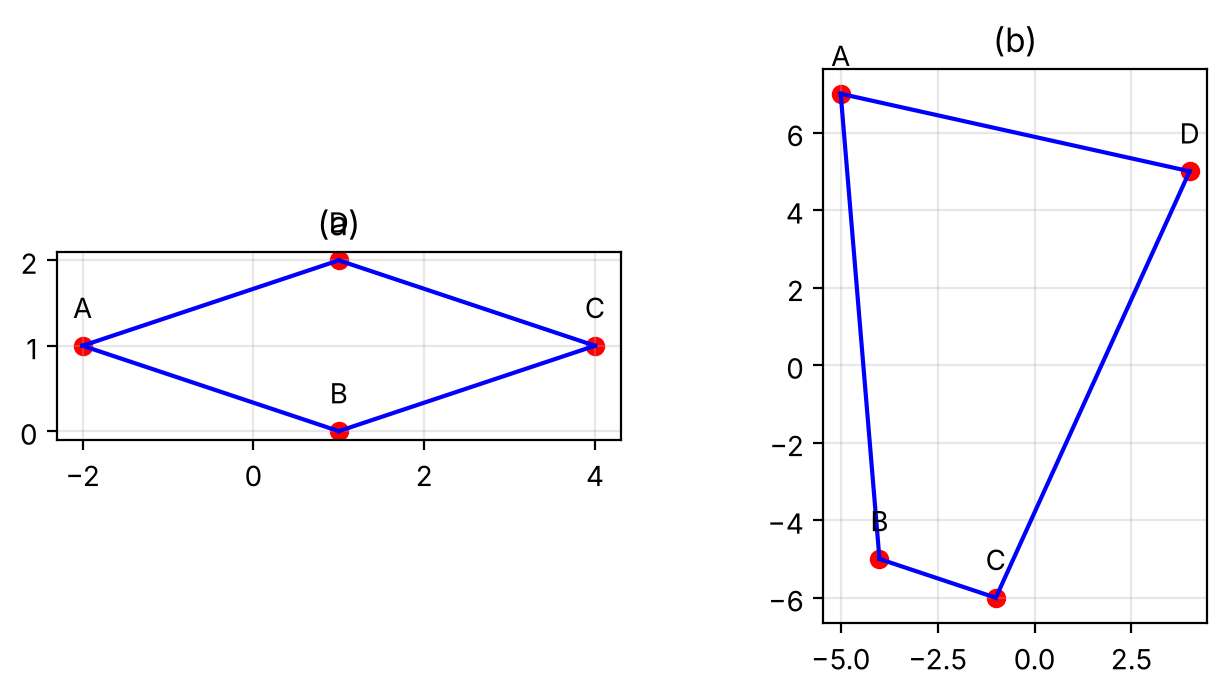
\includegraphics[width=0.95\linewidth]{figs/1.2.15.png}
    \caption{(a) Parallelogram $ABCD$ and (b) quadrilateral $ABCD$}
    \label{fig:quad_q15}
\end{figure}

    \item A plane left 30 minutes late than its scheduled time and in order to reach the destination 1500 km away in time, it had to increase its speed by 100 km/h from the usual speed. Find its usual speed.

\solution
Let the usual speed be $x$ km/h. The delay of $\frac{1}{2}$ hour on $1500$ km gives
\begin{align}
\frac{1500}{x} - \frac{1500}{x+100} = \frac{1}{2} \implies f(x) = x^2 + 100x - 300000 = 0
\end{align}
The speed is the positive root of $f$. With $f'(x) = 2x + 100$, the Newton--Raphson iteration is
\begin{align}
x_{n+1} = x_n - \frac{x_n^2 + 100x_n - 300000}{2x_n + 100}
\end{align}
\par\noindent\hfill\mbox{\textit{(\ref{eq:EE26BTECH11225-newton})}}\par
Starting from $x_0 = 1000$ and from $x_0 = -1000$, the C program gives
\[
\begin{array}{c|r|r}
n & x_n\;(x_0=1000) & x_n\;(x_0=-1000)\\\hline
0 & 1000.000000 & -1000.000000 \\
1 & 619.047619 & -684.210526 \\
2 & 510.591425 & -605.590740 \\
3 & 500.100054 & -600.028129 \\
4 & 500.000009 & -600.000001 \\
5 & 500.000000 & -600.000000 \\
6 & 500.000000 & -600.000000
\end{array}
\]
The iterates settle at $500$ and $-600$. Speed cannot be negative, so the usual speed is $\boxed{500\text{ km/h}}$. This agrees with $f(x) = (x-500)(x+600)$. The C program prints the iterates and checks both roots, and the Python program draws the first three Newton steps as tangent lines using CoordGeo in \figref{fig:newton_q16}.
\begin{lstlisting}[frame=single, basicstyle=\rmfamily, escapeinside={(*@}{@*)}]
(*@\makebox[\dimexpr\linewidth-2\fboxsep-2\fboxrule\relax][c]{codes/1.2.16.c}@*)
\end{lstlisting}
\begin{lstlisting}[frame=single, basicstyle=\rmfamily, escapeinside={(*@}{@*)}]
(*@\makebox[\dimexpr\linewidth-2\fboxsep-2\fboxrule\relax][c]{codes/1.2.16.py}@*)
\end{lstlisting}
\begin{figure}[H]
    \centering
    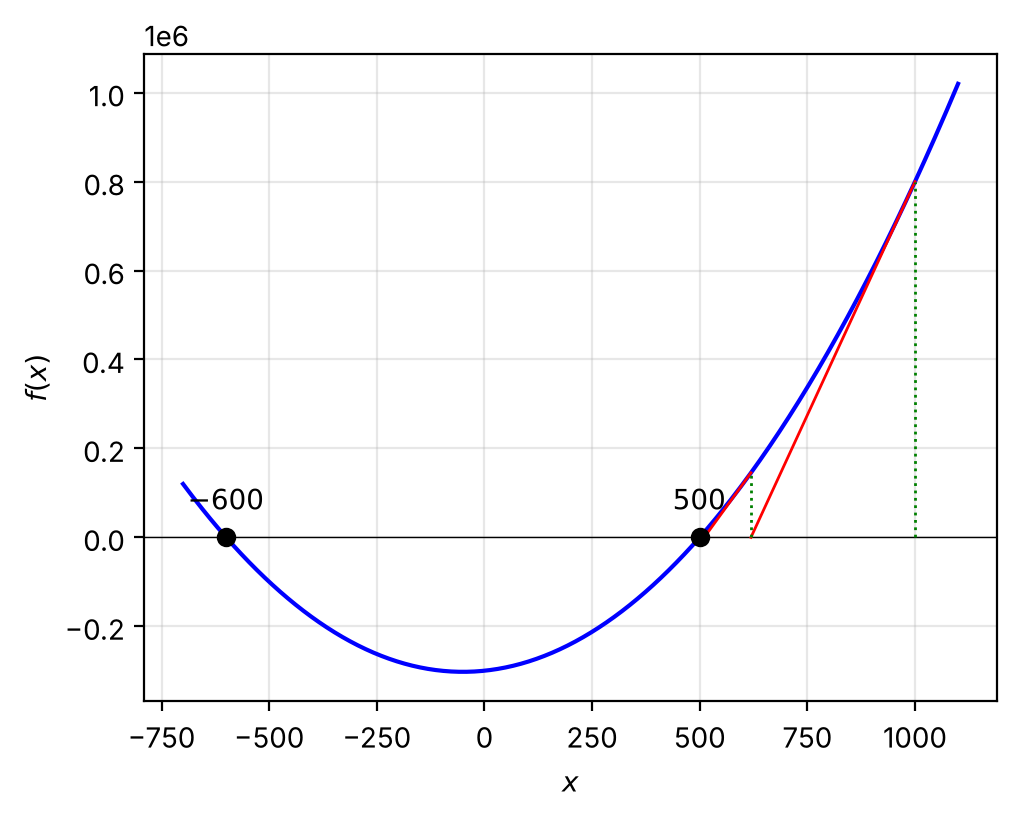
\includegraphics[width=0.65\linewidth]{figs/1.2.16.png}
    \caption{Newton--Raphson steps for $f(x) = x^2 + 100x - 300000$ from $x_0 = 1000$}
    \label{fig:newton_q16}
\end{figure}

    \item 
    \begin{enumerate}[label=(\alph*), leftmargin=1.5em, labelsep=0.5em]
        \item Prove that the area of an equilateral triangle described on one side of a square is equal to half the area of the equilateral triangle described on one of its diagonals.
        
        \vspace{0.5em}
        \begin{center}
            \textbf{OR}
        \end{center}
        \vspace{0.5em}

        \item If the areas of two similar triangles are equal, prove that they are congruent.	\\[2pt]
    \end{enumerate}
    \noindent\textbf{(a) Solution:} Let $ABCD$ be a square of side length $a$.
From \eqref{eq:EE26BTECH11225-pythagoras}, the length of diagonal $AC$ is given by:
\begin{align}
    AC &= \sqrt{a^2 + a^2} = a\sqrt{2}
\end{align}

\begin{center}
    \begin{tikzpicture}[scale=0.9]
        % Square ABCD
        \draw[line width=1.2pt] (0,0) coordinate (B) -- (3,0) coordinate (C) -- (3,3) coordinate (A) -- (0,3) coordinate (D) -- cycle;
        
        % Diagonal AC
        \draw[thick, dashed] (A) -- (C);
        
        % Equilateral Triangle on side BC (BCE)
        \coordinate (E) at (4.5, 2.598);
        \draw[line width=1pt, blue] (B) -- (E) -- (C);
        
        % Equilateral Triangle on diagonal AC (ACF)
        % Angle of AC is -45 deg, side is 3*sqrt(2) = 4.242
        \coordinate (F) at (5.121, 5.121);
        \draw[line width=1pt, red, dashed] (A) -- (F) -- (C);
        
        % Labels
        \node[above left] at (D) {\textbf{D}};
        \node[above left] at (A) {\textbf{A}};
        \node[below left] at (B) {\textbf{B}};
        \node[below right] at (C) {\textbf{C}};
        \node[right, blue] at (E) {\textbf{E}};
        \node[above right, red] at (F) {\textbf{F}};
        
        % Side labels
        \node[below] at (1.5,0) {$a$};
        \node[left] at (0,1.5) {$a$};
    \end{tikzpicture}

    \captionof{figure}{Equilateral triangles $\Delta BCE$ on side $a$ and $\Delta ACF$ on diagonal $a\sqrt{2}$}
    \label{fig:square_triangles_q17}
\end{center} \vspace{2pt}

Let $\Delta BCE$ be the equilateral triangle described on side $BC = a$, and $\Delta ACF$ be the equilateral triangle described on diagonal $AC = a\sqrt{2}$.

Area of an equilateral triangle with side $s$ is given by $\frac{\sqrt{3}}{4} s^2$.

Area of $\Delta BCE$:
\begin{align}
    \text{Area}(\Delta BCE) &= \frac{\sqrt{3}}{4} a^2
\end{align}

Area of $\Delta ACF$:
\begin{align}
    \text{Area}(\Delta ACF) &= \frac{\sqrt{3}}{4} (a\sqrt{2})^2 = \frac{\sqrt{3}}{4} (2a^2) = 2 \left( \frac{\sqrt{3}}{4} a^2 \right) \\
    &\implies \text{Area}(\Delta BCE) = \frac{1}{2} \text{Area}(\Delta ACF)
\end{align}
Hence proved. \\[8pt]
\noindent\textbf{(b) Solution:} Let $\Delta ABC \sim \Delta PQR$ such that $\text{Area}(\Delta ABC) = \text{Area}(\Delta PQR)$.

From \eqref{eq:EE26BTECH11225-area-ratio} (area ratio theorem for similar triangles):
\begin{align}
    \frac{\text{Area}(\Delta ABC)}{\text{Area}(\Delta PQR)} &= \left(\frac{AB}{PQ}\right)^2 = \left(\frac{BC}{QR}\right)^2 = \left(\frac{AC}{PR}\right)^2
\end{align}

Since $\text{Area}(\Delta ABC) = \text{Area}(\Delta PQR)$, the ratio of their areas is $1$:
\begin{align}
    1 = \left(\frac{AB}{PQ}\right)^2 &\implies \frac{AB}{PQ} = 1 \implies AB = PQ \\
    1 = \left(\frac{BC}{QR}\right)^2 &\implies \frac{BC}{QR} = 1 \implies BC = QR \\
    1 = \left(\frac{AC}{PR}\right)^2 &\implies \frac{AC}{PR} = 1 \implies AC = PR
\end{align}

Since all three corresponding sides are equal ($AB = PQ$, $BC = QR$, $AC = PR$), by SSS congruence criterion:
\begin{align}
    \Delta ABC \cong \Delta PQR
\end{align}
Hence proved.
    \item Prove that the lengths of tangents drawn from an external point to a circle are equal.

\solution Let $P$ be an external point to a circle with centre $O$. Let $PA$ and $PB$ be two tangents drawn from $P$ touching the circle at points $A$ and $B$ respectively. Join $OA$, $OB$, and $OP$.

\begin{figure}[H]
    \centering
    \begin{tikzpicture}[scale=0.8]
        % Circle centre and radius
        \coordinate (O) at (0,0);
        \draw[line width=1pt] (O) circle (2cm);
        
        % External point P
        \coordinate (P) at (5,0);
        
        % Tangent points A and B
        \coordinate (A) at (0.8, 1.833);
        \coordinate (B) at (0.8, -1.833);
        
        % Draw radius lines
        \draw[line width=1pt, dashed] (O) -- (A);
        \draw[line width=1pt, dashed] (O) -- (B);
        \draw[line width=1pt, dashed] (O) -- (P);
        
        % Draw tangent lines
        \draw[line width=1pt] (P) -- (A);
        \draw[line width=1pt] (P) -- (B);
        
        % Right angle indicators
        \draw (0.68, 1.56) -- (0.95, 1.44) -- (1.07, 1.71);
        \draw (0.68, -1.56) -- (0.95, -1.44) -- (1.07, -1.71);
        
        % Labels
        \node[left] at (O) {\textbf{O}};
        \node[right] at (P) {\textbf{P}};
        \node[above left] at (A) {\textbf{A}};
        \node[below left] at (B) {\textbf{B}};
    \end{tikzpicture}

    \caption{Tangents $PA$ and $PB$ from external point $P$ to circle with centre $O$}
    \label{fig:tangents_circle}
\end{figure}

In $\Delta OAP$ and $\Delta OBP$:
\begin{align}
    \angle OAP = \angle OBP &= 90^\circ \quad (\text{Radius is perpendicular to tangent, from } \eqref{eq:EE26BTECH11225-tangent-perp}) \\
    OP &= OP \quad (\text{Common hypotenuse}) \\
    OA &= OB \quad (\text{Radii of the same circle})
\end{align}
By RHS congruence criterion:
\begin{align}
    \Delta OAP \cong \Delta OBP &\implies PA = PB
\end{align}
Hence, the lengths of tangents drawn from an external point to a circle are equal.
    \item 
    \begin{enumerate}[label=(\alph*), leftmargin=1.5em, labelsep=0.5em]
        \item If $4 \tan\theta = 3$, evaluate $\left( \frac{4 \sin\theta - \cos\theta + 1}{4 \sin\theta + \cos\theta - 1} \right)$.
        
        \vspace{0.5em}
        \begin{center}
            \textbf{OR}
        \end{center}
        \vspace{0.5em}

        \item If $\tan 2A = \cot(A - 18^\circ)$, where $2A$ is an acute angle, find the value of $A$.	\\[2pt]
        \noindent\textbf{(a) Solution:} Given $4\tan\theta = 3 \implies \tan\theta = \frac{3}{4}$.

Consider a right-angled triangle with opposite side $= 3$ and adjacent side $= 4$.
By Pythagoras theorem, from \eqref{eq:EE26BTECH11225-pythagoras}, the hypotenuse is:
\begin{align}
    \text{Hypotenuse} &= \sqrt{3^2 + 4^2} = \sqrt{9 + 16} = \sqrt{25} = 5
\end{align}

Therefore, from \eqref{eq:EE26BTECH11225-trig-ratios}:
\begin{align}
    \sin\theta &= \frac{3}{5}, \quad \cos\theta = \frac{4}{5}
\end{align}

Substituting these values into the given expression:
\begin{align}
    \frac{4\sin\theta - \cos\theta + 1}{4\sin\theta + \cos\theta - 1} &= \frac{4\left(\frac{3}{5}\right) - \frac{4}{5} + 1}{4\left(\frac{3}{5}\right) + \frac{4}{5} - 1} \\
    &= \frac{\frac{12}{5} - \frac{4}{5} + 1}{\frac{12}{5} + \frac{4}{5} - 1} \\
    &= \frac{\frac{8}{5} + 1}{\frac{16}{5} - 1} \\
    &= \frac{\frac{13}{5}}{\frac{11}{5}} = \frac{13}{11}
\end{align}
Thus, the value of the expression is $\frac{13}{11}$. \\[8pt]
\noindent\textbf{(b) Solution:} Given $\tan 2A = \cot(A - 18^\circ)$.

From \eqref{eq:EE26BTECH11225-complementary}, $\tan \theta = \cot(90^\circ - \theta)$:
\begin{align}
    \cot(90^\circ - 2A) &= \cot(A - 18^\circ)
\end{align}

Equating the angles:
\begin{align}
    90^\circ - 2A &= A - 18^\circ \\
    &\implies 90^\circ + 18^\circ = A + 2A \\
    &\implies 3A = 108^\circ \\
    &\implies A = \frac{108^\circ}{3} = 36^\circ
\end{align}
Thus, the value of $A$ is $36^\circ$.
        
    \end{enumerate}
   \item Find the area of the shaded region in \figref{fig:shaded_q20}, where arcs drawn with centres $A, B, C$ and $D$ intersect in pairs at mid-points $P, Q, R$ and $S$ of the sides $AB, BC, CD$ and $DA$ respectively of a square $ABCD$ of side $12\text{ cm}$. [Use $\pi = 3.14$]

\begin{figure}[H]
\centering
\begin{tikzpicture}[scale=0.35]
    % Coordinates of Square Vertices
    \coordinate (A) at (0, 12);
    \coordinate (B) at (12, 12);
    \coordinate (C) at (12, 0);
    \coordinate (D) at (0, 0);

    % Midpoints
    \coordinate (P) at (6, 12);
    \coordinate (Q) at (12, 6);
    \coordinate (R) at (6, 0);
    \coordinate (S) at (0, 6);

    % Fill Shaded Region (Square minus 4 quadrant arcs)
    \begin{scope}
        \clip (A) -- (B) -- (C) -- (D) -- cycle;
        % Fill the full square first with pattern/color
        \fill[pattern=north east lines, pattern color=black!70] (A) -- (B) -- (C) -- (D) -- cycle;
        
        % Un-clip/white-out the 4 corner circular quadrants
        \fill[white] (A) -- (P) arc (0:-90:6) -- cycle;
        \fill[white] (B) -- (Q) arc (-90:-180:6) -- cycle;
        \fill[white] (C) -- (R) arc (180:90:6) -- cycle;
        \fill[white] (D) -- (S) arc (90:0:6) -- cycle;
    \end{scope}

    % Draw Outer Square
    \draw[line width=1.2pt] (A) -- (B) -- (C) -- (D) -- cycle;

    % Draw Arcs
    \draw[line width=1pt] (P) arc (0:-90:6);
    \draw[line width=1pt] (Q) arc (-90:-180:6);
    \draw[line width=1pt] (R) arc (180:90:6);
    \draw[line width=1pt] (S) arc (90:0:6);

    % Label Vertices
    \node[above left] at (A) {\textbf{A}};
    \node[above right] at (B) {\textbf{B}};
    \node[below right] at (C) {\textbf{C}};
    \node[below left] at (D) {\textbf{D}};

    % Label Midpoints
    \node[above] at (P) {\textbf{P}};
    \node[right] at (Q) {\textbf{Q}};
    \node[below] at (R) {\textbf{R}};
    \node[left] at (S) {\textbf{S}};
\end{tikzpicture}

\caption{Shaded region enclosed by circular arcs in square $ABCD$}
\label{fig:shaded_q20}
\end{figure}		 \vspace{2pt}


\solution Given:
\begin{align}
    \text{Side of square } ABCD \ (s) &= 12\text{ cm}
\end{align}

Since $P, Q, R, S$ are the mid-points of the sides of the square, the radius $r$ of each corner sector is:
\begin{align}
    r &= \frac{12}{2} = 6\text{ cm}
\end{align}

Each corner sector has an angle of $90^\circ$ (since all interior angles of a square are $90^\circ$), making each sector a quadrant of a circle. 

From \eqref{eq:EE26BTECH11225-sector}, combining these $4$ identical quadrants forms $1$ complete circle of radius $r = 6\text{ cm}$:
\begin{align}
    \text{Area of } 4\text{ quadrants} &= \text{Area of } 1\text{ full circle} = \pi r^2 \\
    &= 3.14 \times (6)^2 = 3.14 \times 36 = 113.04\text{ cm}^2
\end{align}

Calculating the area of the square:
\begin{align}
    \text{Area of square } ABCD &= s^2 = (12)^2 = 144\text{ cm}^2
\end{align}

Subtracting the area of the circle from the area of the square gives the area of the shaded region:
\begin{align}
    \text{Area of shaded region} &= \text{Area of square } ABCD - \text{Area of } 4\text{ quadrants} \\
    &= 144 - 113.04 = 30.96\text{ cm}^2
\end{align}

Thus, the area of the shaded region is $30.96\text{ cm}^2$.
	\item 
    \begin{enumerate}[label=(\alph*), leftmargin=1.5em, labelsep=0.5em]
        \item A wooden article was made by scooping out a hemisphere from each end of a solid cylinder, as shown in \figref{fig:wooden_q21}. If the height of the cylinder is $10\text{ cm}$ and its base is of radius $3.5\text{ cm}$, find the total surface area of the article.
        
        \begin{figure}[H]
            \centering
            \begin{tikzpicture}[scale=0.8]
            % Top Scooped Hemisphere Pattern Shading
            \path[pattern=north east lines, pattern color=black!70] 
                (-1.5, 2) arc (180:360:1.5 and 1.5) 
                arc (0:180:1.5 and 0.5) -- cycle;

            % Bottom Scooped Hemisphere Pattern Shading
            \path[pattern=north east lines, pattern color=black!70] 
                (-1.5, -2) arc (180:0:1.5 and 1.5) 
                arc (360:180:1.5 and 0.5) -- cycle;

            % Main Cylinder Body Outline
            \draw[thick] (-1.5, -2) -- (-1.5, 2);
            \draw[thick] (1.5, -2) -- (1.5, 2);
            
            % Top Cylinder Rim
            \draw[thick] (0, 2) ellipse (1.5 and 0.5);
            
            % Bottom Cylinder Rim
            \draw[thick] (0, -2) ellipse (1.5 and 0.5);
            
            % Top Scooped Hemisphere Arc
            \draw[thick] (-1.5, 2) arc (180:360:1.5 and 1.5);
            
            % Bottom Scooped Hemisphere Arc
            \draw[thick] (-1.5, -2) arc (180:0:1.5 and 1.5);
            
        \end{tikzpicture}

            \caption{Wooden article}
            \label{fig:wooden_q21}
        \end{figure}
        
        \vspace{0.5em}
        \begin{center}
            \textbf{OR}
        \end{center}
        \vspace{0.5em}

        \item A heap of rice is in the form of a cone of base diameter $24\text{ m}$ and height $3.5\text{ m}$. Find the volume of the rice. How much canvas cloth is required to just cover the heap?	\\[2pt]
        \noindent\textbf{(a) Solution:} Given radius $r = 3.5\text{ cm} = \frac{7}{2}\text{ cm}$ and height of cylinder $h = 10\text{ cm}$.

From \eqref{eq:EE26BTECH11225-csa-cyl} and \eqref{eq:EE26BTECH11225-csa-hemi}, the total surface area (TSA) of the article consists of the curved surface area (CSA) of the cylinder plus the CSA of two hemispherical ends:
\begin{align}
    \text{TSA} &= \text{CSA of cylinder} + 2 \times (\text{CSA of hemisphere}) \\
    &= 2\pi r h + 2 \times (2\pi r^2) \\
    &= 2\pi r h + 4\pi r^2 \\
    &= 2\pi r (h + 2r)
\end{align}

Substituting $r = \frac{7}{2}$ and $h = 10$:
\begin{align}
    \text{TSA} &= 2 \times \frac{22}{7} \times \frac{7}{2} \left( 10 + 2 \times \frac{7}{2} \right) \\
    &= 22 \times (10 + 7) \\
    &= 22 \times 17 = 374\text{ cm}^2
\end{align}
Thus, the total surface area of the article is $374\text{ cm}^2$. \\[8pt]
\noindent\textbf{(b) Solution:} Given diameter $d = 24\text{ m} \implies \text{radius } r = 12\text{ m}$, and height $h = 3.5\text{ m} = \frac{7}{2}\text{ m}$.

From \eqref{eq:EE26BTECH11225-cone-vol}, the volume of the conical heap of rice is:
\begin{align}
    V &= \frac{1}{3} \pi r^2 h \\
    &= \frac{1}{3} \times \frac{22}{7} \times (12)^2 \times \frac{7}{2} \\
    &= \frac{1}{3} \times \frac{22}{7} \times 144 \times \frac{7}{2} \\
    &= 11 \times 48 = 528\text{ m}^3
\end{align}

To find the canvas cloth required to cover the heap, from \eqref{eq:EE26BTECH11225-cone-csa} we calculate the curved surface area ($\text{CSA} = \pi r l$), where $l$ is the slant height:
\begin{align}
    l &= \sqrt{r^2 + h^2} = \sqrt{12^2 + (3.5)^2} \\
    &= \sqrt{144 + 12.25} = \sqrt{156.25} = 12.5\text{ m}
\end{align}

Area of canvas cloth required:
\begin{align}
    \text{CSA} &= \pi r l \\
    &= \frac{22}{7} \times 12 \times 12.5 \\
    &= \frac{22 \times 150}{7} = \frac{3300}{7} \approx 471.43\text{ m}^2
\end{align}
Thus, the volume of rice is $528\text{ m}^3$ and the area of canvas cloth required is $471.43\text{ m}^2$.     
    \end{enumerate}
    \item The table below shows the salaries of 280 persons:
    \begin{center}
    \begin{tabular}{|c|c|}
    \hline
    \textbf{Salary (in thousand Rs.)} & \textbf{No. of Persons} \\
    \hline
    5--10  & 49  \\
    10--15 & 133 \\
    15--20 & 63  \\
    20--25 & 15  \\
    25--30 & 6   \\
    30--35 & 7   \\
    35--40 & 4   \\
    40--45 & 2   \\
    45--50 & 1   \\
    \hline
    \end{tabular}
    \end{center}
    Calculate the median salary of the data.

\solution Constructing the cumulative frequency table:
\begin{center}
\begin{tabular}{|c|c|c|}
    \hline
    \textbf{Salary (in thousand Rs.)} & \textbf{Frequency ($f$)} & \textbf{Cumulative Frequency ($cf$)} \\ \hline
    5--10  & 49  & 49  \\ \hline
    10--15 & 133 & 182 \\ \hline
    15--20 & 63  & 245 \\ \hline
    20--25 & 15  & 260 \\ \hline
    25--30 & 6   & 266 \\ \hline
    30--35 & 7   & 273 \\ \hline
    35--40 & 4   & 277 \\ \hline
    40--45 & 2   & 279 \\ \hline
    45--50 & 1   & 280 \\ \hline
\end{tabular}
\end{center}
Here, $N = 280 \implies \frac{N}{2} = 140$. \\[2pt]
The cumulative frequency just greater than $140$ is $182$, which corresponds to the median class $10\text{--}15$. \\[2pt]
Lower limit of median class $l = 10$, $cf = 49$, $f = 133$, and class width $h = 5$. From \eqref{eq:EE26BTECH11225-median},
\begin{align}
    \text{Median} &= l + \left(\frac{\frac{N}{2} - cf}{f}\right) \times h \\
    &= 10 + \left(\frac{140 - 49}{133}\right) \times 5 \\
    &= 10 + \left(\frac{91}{133}\right) \times 5 \\
    &= 10 + \frac{455}{133} \approx 10 + 3.42 = 13.42
\end{align}
Thus, the median salary is Rs. $13.42\text{ thousand} = \text{Rs. } 13,420$.The following code computes the median and plots the ogive in \figref{fig:median_q22}.
\begin{lstlisting}[frame=single, basicstyle=\rmfamily, escapeinside={(*@}{@*)}]
(*@\makebox[\dimexpr\linewidth-2\fboxsep-2\fboxrule\relax][c]{codes/1.2.22.py}@*)
\end{lstlisting}
\begin{figure}[H]
    \centering
    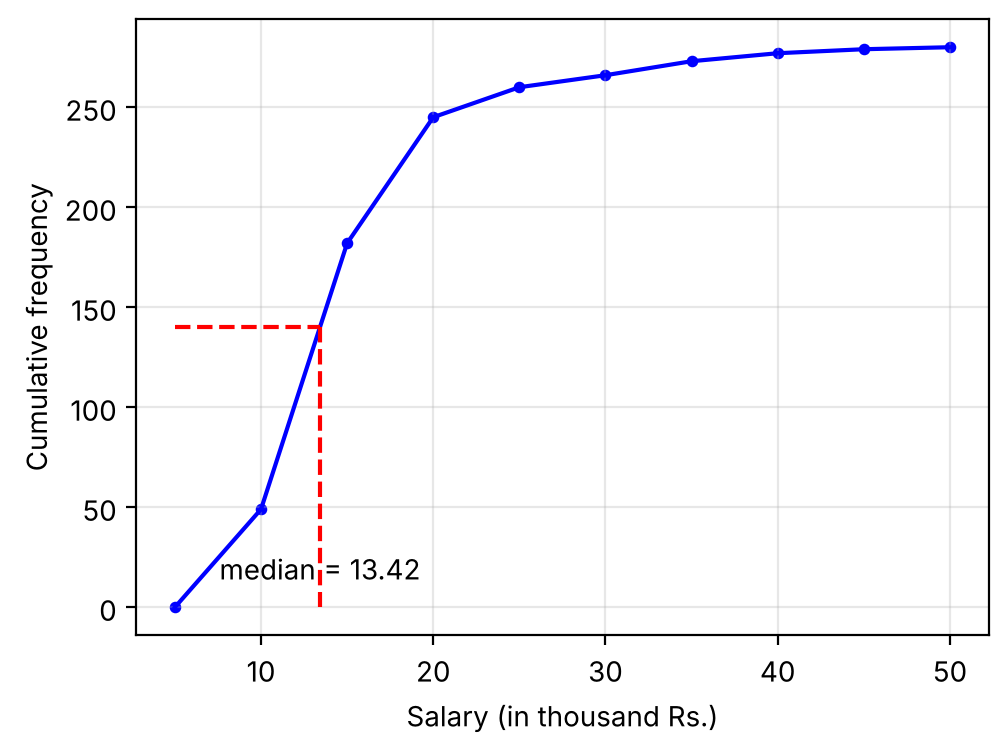
\includegraphics[width=0.70\linewidth]{figs/1.2.22.png}
    \caption{Less than type ogive for the salary data}
    \label{fig:median_q22}
\end{figure}

    \item 
    \begin{enumerate}[label=(\alph*), leftmargin=1.5em, labelsep=0.5em]
        \item A motor boat whose speed is $18\text{ km/h}$ in still water takes $1\text{ hour}$ more to go $24\text{ km}$ upstream than to return downstream to the same spot. Find the speed of the stream.
        
        \vspace{0.5em}
        \begin{center}
            \textbf{OR}
        \end{center}
        \vspace{0.5em}

        \item A train travels at a certain average speed for a distance of $63\text{ km}$ and then travels at a distance of $72\text{ km}$ at an average speed of $6\text{ km/h}$ more than its original speed. If it takes $3\text{ hours}$ to complete total journey, what is the original average speed?
    \end{enumerate}	\vspace{2pt}
    \noindent\textbf{(a) Solution:} Let the speed of the stream be $x\text{ km/h}$.

Given:
\begin{align}
    \text{Speed of boat in still water} &= 18\text{ km/h} \\
    \text{Speed upstream} &= (18 - x)\text{ km/h} \\
    \text{Speed downstream} &= (18 + x)\text{ km/h} \\
    \text{Distance} &= 24\text{ km}
\end{align}

Time taken upstream $t_1 = \frac{24}{18 - x}$ hours, and time taken downstream $t_2 = \frac{24}{18 + x}$ hours.

According to the given condition ($t_1 - t_2 = 1$ hour):
\begin{align}
    \frac{24}{18 - x} - \frac{24}{18 + x} &= 1 \\
    24 \left( \frac{(18 + x) - (18 - x)}{(18 - x)(18 + x)} \right) &= 1 \\
    24 \left( \frac{2x}{324 - x^2} \right) &= 1 \\
    48x &= 324 - x^2 \\
    &\implies x^2 + 48x - 324 = 0
\end{align}

Factoring the quadratic equation:
\begin{align}
    x^2 + 54x - 6x - 324 &= 0 \\
    x(x + 54) - 6(x + 54) &= 0 \\
    (x - 6)(x + 54) &= 0 \\
    &\implies x = 6 \quad \text{or} \quad x = -54
\end{align}

Since speed cannot be negative, $x = 6$.
Thus, the speed of the stream is $6\text{ km/h}$. \\[8pt]
\noindent\textbf{(b) Solution:} Let the original average speed of the train be $x\text{ km/h}$.

Given:
\begin{align}
    \text{Time for first 63 km} &= \frac{63}{x}\text{ hours} \\
    \text{Time for next 72 km} &= \frac{72}{x + 6}\text{ hours}
\end{align}

Total journey time is $3$ hours:
\begin{align}
    \frac{63}{x} + \frac{72}{x + 6} &= 3
\end{align}

Dividing the entire equation by 3:
\begin{align}
    \frac{21}{x} + \frac{24}{x + 6} &= 1 \\
    \frac{21(x + 6) + 24x}{x(x + 6)} &= 1 \\
    21x + 126 + 24x &= x^2 + 6x \\
    45x + 126 &= x^2 + 6x \\
    &\implies x^2 - 39x - 126 = 0
\end{align}

Factoring the quadratic equation:
\begin{align}
    x^2 - 42x + 3x - 126 &= 0 \\
    x(x - 42) + 3(x - 42) &= 0 \\
    (x - 42)(x + 3) &= 0 \\
    &\implies x = 42 \quad \text{or} \quad x = -3
\end{align}

Since speed cannot be negative, $x = 42$.
Thus, the original average speed of the train is $42\text{ km/h}$.The following code verifies both parts.
\begin{lstlisting}[frame=single, basicstyle=\rmfamily, escapeinside={(*@}{@*)}]
(*@\makebox[\dimexpr\linewidth-2\fboxsep-2\fboxrule\relax][c]{codes/1.2.23.py}@*)
\end{lstlisting}

    \item The sum of four consecutive numbers in an AP is 32 and the ratio of the product of the first and the last term to the product of two middle terms is $7 : 15$. Find the numbers.

\solution From \eqref{eq:EE26BTECH11225-ap-four}, let the four consecutive terms of the A.P. be $(a - 3d), (a - d), (a + d),$ and $(a + 3d)$. \\[2pt]
Given that the sum of these four numbers is 32:
\begin{align}
    (a - 3d) + (a - d) + (a + d) + (a + 3d) &= 32 \\
    &\implies 4a = 32 \\
    &\implies a = 8
\end{align}
Also given that the ratio of the product of the first and last terms to the product of the middle terms is $7 : 15$:
\begin{align}
    \frac{(a - 3d)(a + 3d)}{(a - d)(a + d)} &= \frac{7}{15} \\
    &\implies \frac{a^2 - 9d^2}{a^2 - d^2} = \frac{7}{15}
\end{align}
Substituting $a = 8$ ($a^2 = 64$):
\begin{align}
    \frac{64 - 9d^2}{64 - d^2} &= \frac{7}{15} \\
    &\implies 15(64 - 9d^2) = 7(64 - d^2) \\
    &\implies 960 - 135d^2 = 448 - 7d^2 \\
    &\implies 135d^2 - 7d^2 = 960 - 448 \\
    &\implies 128d^2 = 512 \\
    &\implies d^2 = \frac{512}{128} = 4 \\
    &\implies d = \pm 2
\end{align}
Taking $d = 2$:
\begin{align}
    a - 3d &= 8 - 3(2) = 2 \\
    a - d &= 8 - 2 = 6 \\
    a + d &= 8 + 2 = 10 \\
    a + 3d &= 8 + 3(2) = 14
\end{align}
(Taking $d = -2$ gives the same terms in reverse order: $14, 10, 6, 2$).

Thus, the four numbers are $2, 6, 10,$ and $14$.
    \item 
    \begin{enumerate}[label=(\alph*), leftmargin=1.5em, labelsep=0.5em]
        \item In an equilateral $\Delta ABC$, $D$ is a point on side $BC$ such that $BD = \frac{1}{3}BC$. Prove that $9(AD)^2 = 7(AB)^2$.
        
        \vspace{0.5em}
        \begin{center}
            \textbf{OR}
        \end{center}
        \vspace{0.5em}

        \item Prove that, in a right triangle, the square on the hypotenuse is equal to the sum of the squares on the other two sides.
    \end{enumerate}	\vspace{2pt}
    \noindent\textbf{(a) Solution:} Let $\Delta ABC$ be an equilateral triangle with side length $AB = BC = CA = a$.
Draw $AE \perp BC$. In an equilateral triangle, the altitude bisects the base, so:
\begin{align}
    BE = EC = \frac{a}{2}
\end{align}

Given $BD = \frac{1}{3}BC = \frac{a}{3}$.

Now, calculate $DE$:
\begin{align}
    DE &= BE - BD = \frac{a}{2} - \frac{a}{3} = \frac{a}{6}
\end{align}

In right $\Delta AEB$, by Pythagoras theorem, from \eqref{eq:EE26BTECH11225-pythagoras}:
\begin{align}
    AE^2 &= AB^2 - BE^2 = a^2 - \left(\frac{a}{2}\right)^2 = a^2 - \frac{a^2}{4} = \frac{3a^2}{4}
\end{align}

In right $\Delta AED$, by Pythagoras theorem, from \eqref{eq:EE26BTECH11225-pythagoras}:
\begin{align}
    AD^2 &= AE^2 + DE^2 \\
    AD^2 &= \frac{3a^2}{4} + \left(\frac{a}{6}\right)^2 \\
    AD^2 &= \frac{3a^2}{4} + \frac{a^2}{36} \\
    AD^2 &= \frac{27a^2 + a^2}{36} = \frac{28a^2}{36} = \frac{7a^2}{9} \\
    &\implies 9(AD)^2 = 7a^2
\end{align}

Since $a = AB$:
\begin{align}
    9(AD)^2 = 7(AB)^2
\end{align}
Hence proved. \\[8pt]
\noindent\textbf{(b) Solution:} Consider a right-angled triangle $ABC$, right-angled at $B$.

\textbf{To prove:} $AC^2 = AB^2 + BC^2$.

\textbf{Construction:} Draw $BD \perp AC$.

In $\Delta ADB$ and $\Delta ABC$:
\begin{align}
    \angle ADB &= \angle ABC = 90^\circ \\
    \angle A &= \angle A \quad \text{(Common angle)}
\end{align}
By AA similarity criterion, $\Delta ADB \sim \Delta ABC$.
Therefore, ratio of corresponding sides is equal:
\begin{align}
    \frac{AD}{AB} = \frac{AB}{AC} &\implies AB^2 = AD \times AC \label{eq:EE26BTECH11225-pyth-1}
\end{align}

In $\Delta BDC$ and $\Delta ABC$:
\begin{align}
    \angle BDC &= \angle ABC = 90^\circ \\
    \angle C &= \angle C \quad \text{(Common angle)}
\end{align}
By AA similarity criterion, $\Delta BDC \sim \Delta ABC$.
Therefore:
\begin{align}
    \frac{DC}{BC} = \frac{BC}{AC} &\implies BC^2 = DC \times AC \label{eq:EE26BTECH11225-pyth-2}
\end{align}

Adding \eqref{eq:EE26BTECH11225-pyth-1} and \eqref{eq:EE26BTECH11225-pyth-2}:
\begin{align}
    AB^2 + BC^2 &= (AD \times AC) + (DC \times AC) \\
    &= AC(AD + DC)
\end{align}

Since $AD + DC = AC$:
\begin{align}
    AB^2 + BC^2 &= AC \times AC = AC^2
\end{align}
Hence proved.
    
    \item Draw a triangle $ABC$ with $BC = 6\text{ cm}$, $AB = 5\text{ cm}$ and $\angle ABC = 60^\circ$. Then construct a triangle whose sides are $\frac{3}{4}$ of the corresponding sides of $\triangle ABC$.
\solution
Steps of construction:
\begin{enumerate}[label=(\roman*), leftmargin=1.5em, labelsep=0.5em]
    \item Draw $BC = 6\text{ cm}$.
    \item At $B$, draw ray $BY$ with $\angle CBY = 60^\circ$. With centre $B$ and radius $5\text{ cm}$, cut $BY$ at $A$. Join $AC$.
    \item Below $BC$, draw a ray $BX$ making an acute angle $\angle CBX$ with $BC$.
    \item Along $BX$, mark four points $B_1, B_2, B_3, B_4$ such that $BB_1 = B_1B_2 = B_2B_3 = B_3B_4$.
    \item Join $B_4C$. Through $B_3$, draw $B_3C' \parallel B_4C$ meeting $BC$ at $C'$.
    \item Through $C'$, draw $C'A' \parallel CA$ meeting $BA$ at $A'$.
\end{enumerate}
Then $\Delta A'BC'$ is the required triangle. \\
\textbf{Justification:} Since $B_3C' \parallel B_4C$, by the basic proportionality theorem
\begin{align}
    \frac{BC'}{BC} = \frac{BB_3}{BB_4} = \frac{3}{4}
\end{align}
Since $C'A' \parallel CA$, $\Delta A'BC' \sim \Delta ABC$, so
\begin{align}
    \frac{A'B}{AB} = \frac{BC'}{BC} = \frac{A'C'}{AC} = \frac{3}{4}
\end{align}
The following code verifies the construction and generates \figref{fig:construction_q26}.
\begin{lstlisting}[frame=single, basicstyle=\rmfamily, escapeinside={(*@}{@*)}]
(*@\makebox[\dimexpr\linewidth-2\fboxsep-2\fboxrule\relax][c]{codes/1.2.26.py}@*)
\end{lstlisting}
\begin{figure}[H]
    \centering
    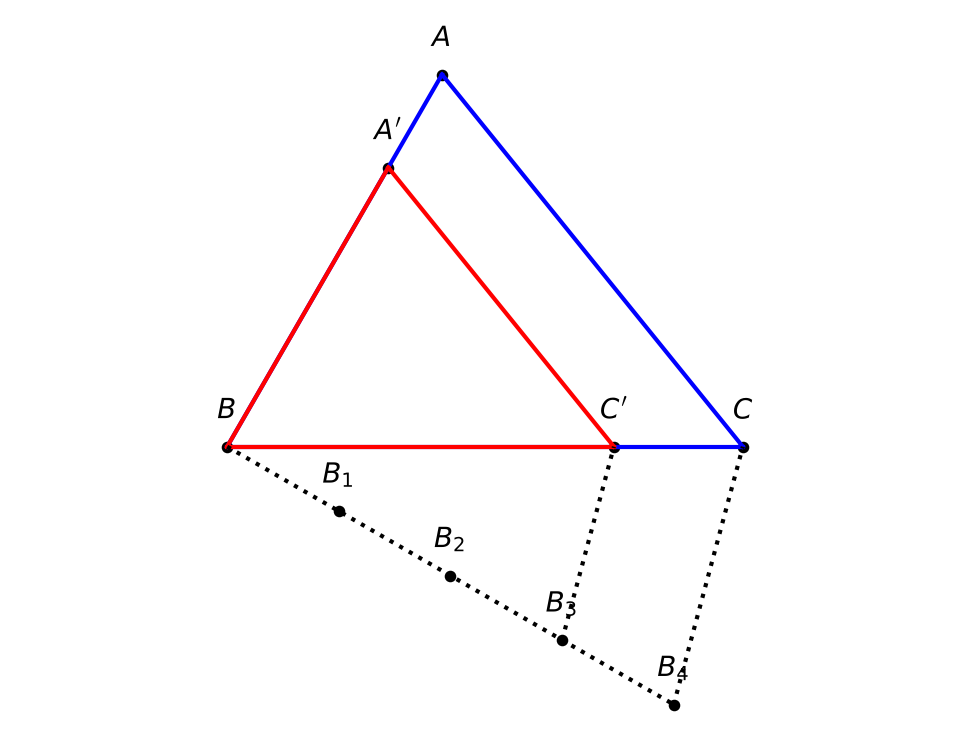
\includegraphics[width=0.75\linewidth]{figs/1.2.26.png}
    \caption{Construction of $\Delta A'BC'$}
    \label{fig:construction_q26}
\end{figure}

    \item Prove that:
    \[
    \frac{\sin A - 2\sin^3 A}{2\cos^3 A - \cos A} = \tan A.
    \]


\solution Taking the Left Hand Side (LHS):
\begin{align}
    \text{LHS} &= \frac{\sin A - 2\sin^3 A}{2\cos^3 A - \cos A} \\
    &= \frac{\sin A (1 - 2\sin^2 A)}{\cos A (2\cos^2 A - 1)}
\end{align}
From \eqref{eq:EE26BTECH11225-trig-1}, $\sin^2 A + \cos^2 A = 1 \implies 1 = \sin^2 A + \cos^2 A$:
\begin{align}
    1 - 2\sin^2 A &= (\sin^2 A + \cos^2 A) - 2\sin^2 A \\
    &= \cos^2 A - \sin^2 A \\
    2\cos^2 A - 1 &= 2\cos^2 A - (\sin^2 A + \cos^2 A) \\
    &= \cos^2 A - \sin^2 A
\end{align}
Substituting these into the expression:
\begin{align}
    \text{LHS} &= \frac{\sin A (\cos^2 A - \sin^2 A)}{\cos A (\cos^2 A - \sin^2 A)} \\
    &= \frac{\sin A}{\cos A} \\
    &= \tan A = \text{RHS}
\end{align}
Hence proved.The following code verifies the identity numerically and plots both sides in \figref{fig:identity_q27}.
\begin{lstlisting}[frame=single, basicstyle=\rmfamily, escapeinside={(*@}{@*)}]
(*@\makebox[\dimexpr\linewidth-2\fboxsep-2\fboxrule\relax][c]{codes/1.2.27.py}@*)
\end{lstlisting}
\begin{figure}[H]
    \centering
    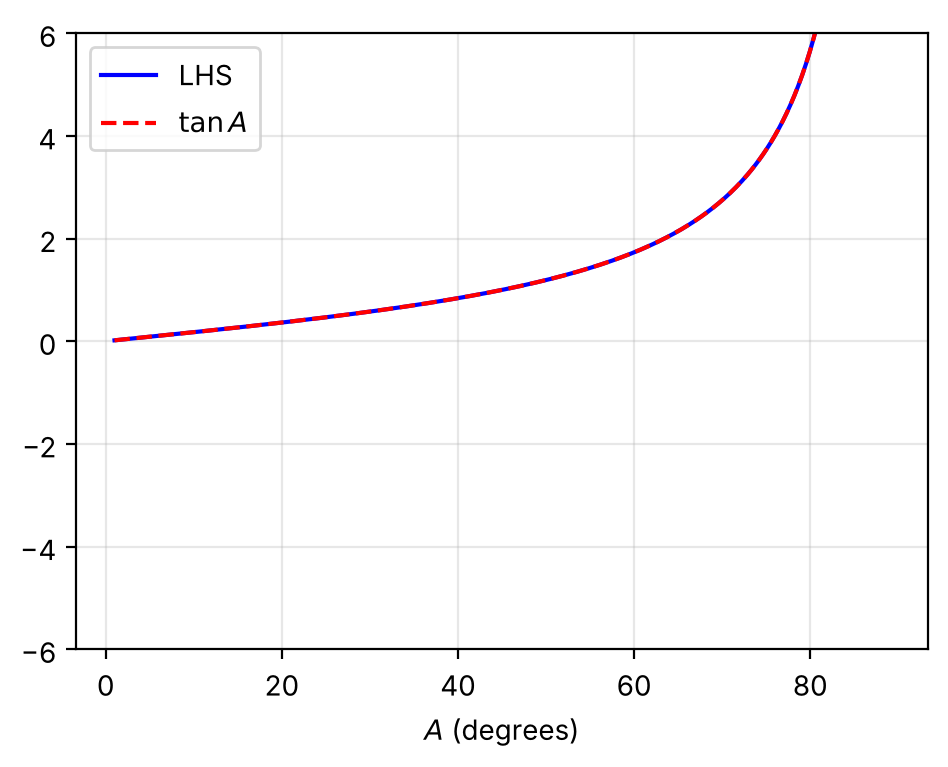
\includegraphics[width=0.70\linewidth]{figs/1.2.27.png}
    \caption{Plot of LHS and $\tan A$}
    \label{fig:identity_q27}
\end{figure}

    \item The diameters of the lower and upper ends of a bucket in the form of a frustum of a cone are 10 cm and 30 cm respectively. If its height is 24 cm, find:
\newline
    (i) The area of the metal sheet used to make the bucket.
\newline
    (ii) Why we should avoid the bucket made by ordinary plastic? [Use $\pi = 3.14$]

\solution Given:
Upper radius $R = \frac{30}{2} = 15\text{ cm}$, lower radius $r = \frac{10}{2} = 5\text{ cm}$, height $h = 24\text{ cm}$. \\[4pt]
From \eqref{eq:EE26BTECH11225-frustum-l}, the slant height $l$ of the frustum is:
\begin{align}
    l &= \sqrt{h^2 + (R - r)^2} \\
    &= \sqrt{24^2 + (15 - 5)^2} \\
    &= \sqrt{576 + 10^2} = \sqrt{576 + 100} = \sqrt{676} = 26\text{ cm}
\end{align}
(i) From \eqref{eq:EE26BTECH11225-frustum-area}, area of the metal sheet used = Curved Surface Area + Area of bottom circular base:
\begin{align}
    \text{Area} &= \pi(R + r)l + \pi r^2 \\
    &= \pi \left[ (15 + 5) \times 26 + 5^2 \right] \\
    &= \pi (20 \times 26 + 25) \\
    &= \pi (520 + 25) = 545 \pi \\
    &= 545 \times 3.14 = 1711.3\text{ cm}^2
\end{align}
Thus, the area of the metal sheet used is $1711.3\text{ cm}^2$. \\[6pt]
(ii) Plastic buckets should be avoided because ordinary plastic is non-biodegradable and causes environmental pollution. Additionally, plastics may leach toxic chemicals when stored with hot water or food items.
    \item As observed from the top of a 100 m high lighthouse from sea level, the angles of depression of two ships are $30^\circ$ and $45^\circ$. If one ship is exactly behind the other on the same side of the lighthouse, find the distance between the two ships. [Use $\sqrt{3} = 1.732$]

\solution Let $AB$ be the lighthouse of height $h = 100\text{ m}$, and $C, D$ be the two ships on the same side of the lighthouse such that the angles of depression are $45^\circ$ and $30^\circ$ respectively. Let $BC = x\text{ m}$ and $CD = y\text{ m}$ (the distance between the two ships).

\begin{center}
    \begin{tikzpicture}[scale=0.85]
        % Horizontal ground/sea level
        \draw[thick] (-0.5,0) -- (6.5,0);
        
        % Lighthouse AB
        \draw[line width=1.2pt] (0,0) -- (0,3.5) node[above] {\textbf{A}};
        \node[below] at (0,0) {\textbf{B}};
        \node[left] at (0,1.75) {$100\text{ m}$};
        
        % Ships C and D
        \coordinate (C) at (3.5,0);
        \coordinate (D) at (6,0);
        \node[below] at (C) {\textbf{C}};
        \node[below] at (D) {\textbf{D}};
        
        % Lines of sight
        \draw[line width=1pt] (0,3.5) -- (3.5,0);
        \draw[line width=1pt] (0,3.5) -- (6,0);
        
        % Horizontal reference line at top for angles of depression
        \draw[dashed] (0,3.5) -- (6.5,3.5) node[right] {\small Horizontal};
        
        % Angles of elevation (alternate interior to angles of depression)
        \draw (2.9,0) arc (180:135:0.6);
        \node at (2.6,0.3) {\small $45^\circ$};
        
        \draw (5.3,0) arc (180:150:0.7);
        \node at (4.9,0.25) {\small $30^\circ$};
        
        % Distance labels
        \draw[<->] (0,-0.6) -- (3.5,-0.6) node[midway,below] {$x$};
        \draw[<->] (3.5,-0.6) -- (6,-0.6) node[midway,below] {$y$};
    \end{tikzpicture}

    \captionof{figure}{Lighthouse $AB$ with ships $C$ and $D$}
    \label{fig:lighthouse_q29}
\end{center}

In right triangle $\Delta ABC$, from \eqref{eq:EE26BTECH11225-trig-ratios}:
\begin{align}
    \tan 45^\circ &= \frac{AB}{BC} \\
    &\implies 1 = \frac{100}{x} \\
    &\implies x = 100\text{ m}
\end{align}

In right triangle $\Delta ABD$, from \eqref{eq:EE26BTECH11225-trig-ratios}:
\begin{align}
    \tan 30^\circ &= \frac{AB}{BD} = \frac{AB}{x + y} \\
    &\implies \frac{1}{\sqrt{3}} = \frac{100}{100 + y} \\
    &\implies 100 + y = 100\sqrt{3} \\
    &\implies y = 100\sqrt{3} - 100 \\
    &\implies y = 100(\sqrt{3} - 1) \\
    &\implies y = 100(1.732 - 1) = 100(0.732) = 73.2\text{ m}
\end{align}
Thus, the distance between the two ships is $73.2\text{ m}$.
    \item 
    \begin{enumerate}[label=(\alph*), leftmargin=1.5em, labelsep=0.5em]
    		\item The mean of the following distribution is $18$. Find the frequency $f$ of the class $19\text{--}21$.
    
    \begin{center}
    \begin{tabular}{|c|c|c|c|c|c|c|c|}
        \hline
        \textbf{Class} & 11--13 & 13--15 & 15--17 & 17--19 & 19--21 & 21--23 & 23--25 \\ \hline
        \textbf{Frequency} & 3 & 6 & 9 & 13 & $f$ & 5 & 4 \\ \hline
    \end{tabular}
    \end{center}
        
        \vspace{0.5em}
        \begin{center}
            \textbf{OR}
        \end{center}
        \vspace{0.5em}

        \item The following distribution gives the daily income of $50$ workers of a factory:

\begin{center}
\begin{tabular}{|c|c|c|c|c|c|}
    \hline
    \textbf{Daily Income (in Rs.)} & 100--120 & 120--140 & 140--160 & 160--180 & 180--200 \\ \hline
    \textbf{Number of workers} & 12 & 14 & 8 & 6 & 10 \\ \hline
\end{tabular}
\end{center}

Convert the distribution above to a less than type cumulative frequency distribution and draw its ogive.
    \end{enumerate}	\vspace{2pt}
    \noindent\textbf{(a) Solution:} Constructing the frequency table to calculate the mean:

\begin{center}
\begin{tabular}{|c|c|c|c|}
    \hline
    \textbf{Class Interval} & \textbf{Class Mark ($x_i$)} & \textbf{Frequency ($f_i$)} & \textbf{$f_i x_i$} \\
    \hline
    11--13 & 12 & 3 & 36 \\
    13--15 & 14 & 6 & 84 \\
    15--17 & 16 & 9 & 144 \\
    17--19 & 18 & 13 & 234 \\
    19--21 & 20 & $f$ & $20f$ \\
    21--23 & 22 & 5 & 110 \\
    23--25 & 24 & 4 & 96 \\
    \hline
    \textbf{Total} & & $\sum f_i = 40 + f$ & $\sum f_i x_i = 704 + 20f$ \\
    \hline
\end{tabular}
\end{center}

Given Mean ($\bar{x}$) $= 18$. From \eqref{eq:EE26BTECH11225-mean}, the mean is:
\begin{align}
    \bar{x} &= \frac{\sum f_i x_i}{\sum f_i} \\
    18 &= \frac{704 + 20f}{40 + f} \\
    18(40 + f) &= 704 + 20f \\
    720 + 18f &= 704 + 20f \\
    720 - 704 &= 20f - 18f \\
    16 &= 2f \\
    &\implies f = \frac{16}{2} = 8
\end{align}
Thus, the missing frequency $f$ is $8$. \\[8pt]
\noindent\textbf{(b) Solution:} Converting the given data into a ``less than type'' cumulative frequency distribution:

\begin{center}
\begin{tabular}{|c|c|}
    \hline
    \textbf{Daily Income (in Rs.)} & \textbf{Cumulative Frequency (cf)} \\
    \hline
    Less than 120 & 12 \\
    Less than 140 & 26 \quad ($12 + 14$) \\
    Less than 160 & 34 \quad ($26 + 8$) \\
    Less than 180 & 40 \quad ($34 + 6$) \\
    Less than 200 & 50 \quad ($40 + 10$) \\
    \hline
\end{tabular}
\end{center}

To plot the ``less than type'' ogive, plot the points $(100, 0)$ (the lower limit of the first class, where the cumulative frequency is $0$), $(120, 12)$, $(140, 26)$, $(160, 34)$, $(180, 40)$, and $(200, 50)$ on a graph with upper limits on the $x$-axis and cumulative frequencies on the $y$-axis, and join them with a smooth freehand curve. The following code verifies part (a) and plots the ogive in \figref{fig:ogive_q30}.

\begin{lstlisting}[frame=single, basicstyle=\rmfamily, escapeinside={(*@}{@*)}]
(*@\makebox[\dimexpr\linewidth-2\fboxsep-2\fboxrule\relax][c]{codes/1.2.30.py}@*)
\end{lstlisting}
\begin{figure}[H]
    \centering
    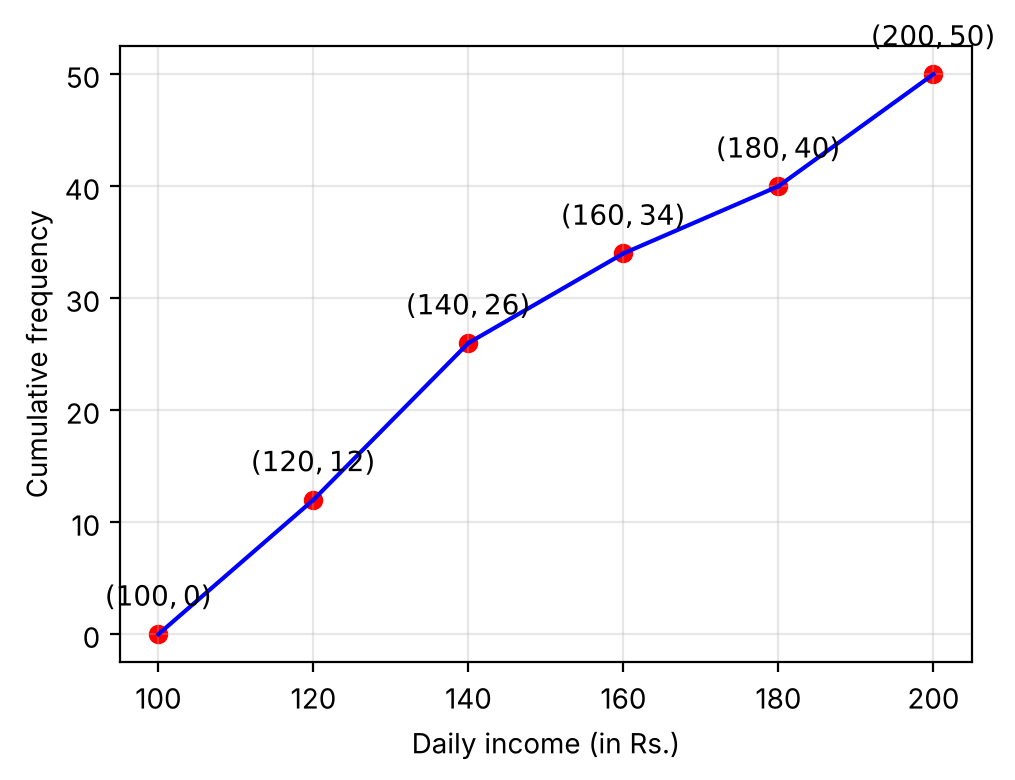
\includegraphics[width=0.70\linewidth]{figs/1.2.30.png}
    \caption{Less than type ogive for daily income distribution}
    \label{fig:ogive_q30}
\end{figure}
\end{enumerate}

\clearpage

\section{CBSE CLASS-12 MATH 2018}
\subsection{Formulae}
\begin{enumerate}[label=\thesubsection.\arabic*, ref=\thesubsection.\theenumi]

\item Determinant properties for square matrices $\vec{A}, \vec{B}$ of order $n$ and a scalar $k$:
\begin{align}
	\begin{split}
		\mydet{\vec{A}\vec{B}} &= \mydet{\vec{A}}\mydet{\vec{B}}
		\\
		\mydet{\vec{A}^{\top}} &= \mydet{\vec{A}}
		\\
		\mydet{k\vec{A}} &= k^n\mydet{\vec{A}}
	\end{split}
	\label{eq:EE26BTECH11225-det}
\end{align}
\solution
If $\vec{A}$ is invertible, it is a product of elementary matrices,
\begin{align}
	\vec{A} = \vec{E}_1\vec{E}_2\cdots\vec{E}_m
\end{align}
and for a single elementary matrix $\mydet{\vec{E}\vec{B}} = \mydet{\vec{E}}\mydet{\vec{B}}$. Repeating this $m$ times,
\begin{align}
	\mydet{\vec{A}\vec{B}} = \mydet{\vec{E}_1}\cdots\mydet{\vec{E}_m}\mydet{\vec{B}}
	= \mydet{\vec{A}}\mydet{\vec{B}}
\end{align}
For the transpose, $\vec{A}^{\top} = \vec{E}_m^{\top}\cdots\vec{E}_1^{\top}$ and $\mydet{\vec{E}^{\top}} = \mydet{\vec{E}}$ for any elementary matrix, so
$\mydet{\vec{A}^{\top}} = \mydet{\vec{A}}$. If $\vec{A}$ is singular, so is $\vec{A}^{\top}$ and both determinants are $0$. Finally, $k\vec{A} = \brak{k\vec{I}}\vec{A}$ with $\mydet{k\vec{I}} = k^n$, yielding \eqref{eq:EE26BTECH11225-det}.

\item Inverse trigonometric identities:
\begin{align}
	\cos^{-1}\brak{\cos t} &= t, \quad t \in \sbrak{0, \pi}
	\label{eq:EE26BTECH11225-invtrig-1}
	\\
	\tan^{-1}a + \tan^{-1}b &= \tan^{-1}\frac{a + b}{1 - ab}, \quad ab < 1
	\label{eq:EE26BTECH11225-invtrig-2}
	\\
	\tan^{-1}x + \cot^{-1}x &= \frac{\pi}{2}
	\label{eq:EE26BTECH11225-invtrig-3}
	\\
	\sin^{-1}x &= \tan^{-1}\frac{x}{\sqrt{1 - x^2}}, \quad \abs{x} < 1
	\label{eq:EE26BTECH11225-invtrig-4}
\end{align}
\solution
\eqref{eq:EE26BTECH11225-invtrig-1} follows from the definition of the principal value, $\cos^{-1}:\sbrak{-1,1} \to \sbrak{0,\pi}$.
\\
For \eqref{eq:EE26BTECH11225-invtrig-2}, let $\alpha = \tan^{-1}a$ and $\beta = \tan^{-1}b$, both in $\brak{-\frac{\pi}{2}, \frac{\pi}{2}}$. Then
\begin{align}
	\tan\brak{\alpha + \beta} = \frac{\tan\alpha + \tan\beta}{1 - \tan\alpha\tan\beta} = \frac{a + b}{1 - ab}
\end{align}
Also $\cos\brak{\alpha + \beta} = \cos\alpha\cos\beta\brak{1 - ab} > 0$ for $ab < 1$, and $\abs{\alpha + \beta} < \pi$, so $\alpha + \beta \in \brak{-\frac{\pi}{2}, \frac{\pi}{2}}$, the principal range of $\tan^{-1}$.
\\
For \eqref{eq:EE26BTECH11225-invtrig-3}, let $\theta = \tan^{-1}x$. Using $\cot\brak{90^\circ - \theta} = \tan\theta = x$ with $\frac{\pi}{2} - \theta \in \brak{0, \pi}$, the principal range of $\cot^{-1}$,
\begin{align}
	\cot^{-1}x = \frac{\pi}{2} - \theta
\end{align}
For \eqref{eq:EE26BTECH11225-invtrig-4}, let $\theta = \sin^{-1}x \in \brak{-\frac{\pi}{2}, \frac{\pi}{2}}$. Then $\cos\theta = \sqrt{1 - x^2} > 0$ and
\begin{align}
	\tan\theta = \frac{x}{\sqrt{1 - x^2}}
	\implies \theta = \tan^{-1}\frac{x}{\sqrt{1 - x^2}}
\end{align}

\item Angle $\theta$ between a line with direction vector $\vec{b}$ and a plane with normal vector $\vec{n}$:
\begin{align}
	\sin\theta = \frac{\abs{\vec{b}^{\top}\vec{n}}}{\norm{\vec{b}}\norm{\vec{n}}}
	\label{eq:EE26BTECH11225-lineplane}
\end{align}
\solution
The normal is perpendicular to the plane, so if $\phi$ is the angle between $\vec{b}$ and $\vec{n}$, then $\theta = 90^\circ - \phi$ (or its supplement). From \eqref{eq:EE26BTECH11225-dot},
\begin{align}
	\sin\theta = \abs{\cos\phi} = \frac{\abs{\vec{b}^{\top}\vec{n}}}{\norm{\vec{b}}\norm{\vec{n}}}
\end{align}

\item For vectors $\vec{a}$, $\vec{b}$ with angle $\theta$ between them:
\begin{align}
	\vec{a}^{\top}\vec{b} &= \norm{\vec{a}}\norm{\vec{b}}\cos\theta
	\label{eq:EE26BTECH11225-dot}
	\\
	\norm{\vec{a} \times \vec{b}} &= \norm{\vec{a}}\norm{\vec{b}}\sin\theta
	\label{eq:EE26BTECH11225-cross}
\end{align}
\solution
The third side of the triangle formed by $\vec{a}$ and $\vec{b}$ is $\vec{a} - \vec{b}$. From the cosine rule and by expanding the norm,
\begin{align}
	\norm{\vec{a} - \vec{b}}^2 &= \norm{\vec{a}}^2 + \norm{\vec{b}}^2 - 2\norm{\vec{a}}\norm{\vec{b}}\cos\theta
	\\
	\norm{\vec{a} - \vec{b}}^2 &= \norm{\vec{a}}^2 + \norm{\vec{b}}^2 - 2\vec{a}^{\top}\vec{b}
\end{align}
yielding \eqref{eq:EE26BTECH11225-dot}. Using Lagrange's identity,
\begin{align}
	\norm{\vec{a} \times \vec{b}}^2 = \norm{\vec{a}}^2\norm{\vec{b}}^2 - \brak{\vec{a}^{\top}\vec{b}}^2
	= \norm{\vec{a}}^2\norm{\vec{b}}^2\brak{1 - \cos^2\theta}
\end{align}
which yields \eqref{eq:EE26BTECH11225-cross} since $\sin\theta \geq 0$ for $\theta \in \sbrak{0, \pi}$.

\item A binary operation $*$ on a set $S$ requires $a * b \in S$ for all $a, b \in S$ (closure). It is commutative if
\begin{align}
	a * b = b * a \quad \forall\, a, b \in S
	\label{eq:EE26BTECH11225-binop}
\end{align}
\solution
For a finite set $S = \cbrak{a_1, \ldots, a_m}$, form the operation table
\begin{align}
	\vec{T} = \sbrak{T_{ij}}, \quad T_{ij} = a_i * a_j
\end{align}
The operation is closed if every entry of $\vec{T}$ lies in $S$. It is commutative if
\begin{align}
	T_{ij} = T_{ji} \quad \forall\, i, j
	\iff \vec{T} = \vec{T}^{\top}
\end{align}
which is \eqref{eq:EE26BTECH11225-binop}.

\item Homogeneous differential equation $\frac{dy}{dx} = f\brak{\frac{y}{x}}$: substitute $y = vx$,
\begin{align}
	\frac{dy}{dx} = v + x\frac{dv}{dx}
	\label{eq:EE26BTECH11225-homog}
\end{align}
\solution
Differentiating $y = vx$ using the product rule yields \eqref{eq:EE26BTECH11225-homog}. Substituting in the equation, the variables separate,
\begin{align}
	x\frac{dv}{dx} = f\brak{v} - v
	\implies \int\frac{dv}{f\brak{v} - v} = \ln\abs{x} + C
\end{align}
Finally $v$ is replaced by $\frac{y}{x}$.

\item Differential equation of a family of curves with $n$ arbitrary constants $c_1, \ldots, c_n$:
\begin{align}
	F\brak{x, y, c_1, \ldots, c_n} = 0
	\implies G\brak{x, y, y^{\prime}, \ldots, y^{\brak{n}}} = 0
	\label{eq:EE26BTECH11225-family}
\end{align}
\solution
Differentiating $F = 0$ $n$ times gives $n + 1$ equations in the $n$ constants. Eliminating $c_1, \ldots, c_n$ from them leaves an equation of order $n$. For example, for
\begin{align}
	y = c_1\cos\brak{\alpha x} + c_2\sin\brak{\alpha x}
\end{align}
differentiating twice,
\begin{align}
	y^{\prime\prime} = -\alpha^2\brak{c_1\cos\brak{\alpha x} + c_2\sin\brak{\alpha x}}
	\implies y^{\prime\prime} = -\alpha^2 y
\end{align}
which has no arbitrary constants left.

\item Points $A, B, C$ are collinear if $\vec{C} - \vec{B} = k\brak{\vec{B} - \vec{A}}$. Points $A, B, C, D$ are coplanar if
\begin{align}
	\rank\myvec{\vec{B} - \vec{A} & \vec{C} - \vec{A}} &= 1
	\label{eq:EE26BTECH11225-collinear}
	\\
	\det\myvec{\vec{B} - \vec{A} & \vec{C} - \vec{A} & \vec{D} - \vec{A}} &= 0
	\label{eq:EE26BTECH11225-coplanar}
\end{align}
\solution
If $\vec{C} - \vec{B} = k\brak{\vec{B} - \vec{A}}$, then
\begin{align}
	\vec{C} - \vec{A} = \brak{\vec{C} - \vec{B}} + \brak{\vec{B} - \vec{A}} = \brak{k + 1}\brak{\vec{B} - \vec{A}}
\end{align}
so the two columns are linearly dependent, yielding \eqref{eq:EE26BTECH11225-collinear}. Similarly, if the points are coplanar, then
\begin{align}
	\vec{D} - \vec{A} = \alpha\brak{\vec{B} - \vec{A}} + \beta\brak{\vec{C} - \vec{A}}
\end{align}
so the third column is a combination of the first two. Subtracting this combination from the third column leaves a zero column, so the determinant vanishes, yielding \eqref{eq:EE26BTECH11225-coplanar}. Geometrically, the determinant is the volume of the parallelepiped on the three vectors.

\item Standard integrals:
\begin{align}
	\int e^x\sbrak{f\brak{x} + f^{\prime}\brak{x}}dx &= e^x f\brak{x} + C
	\label{eq:EE26BTECH11225-expint}
	\\
	\int \frac{du}{\sqrt{a^2 - u^2}} &= \sin^{-1}\frac{u}{a} + C
	\label{eq:EE26BTECH11225-sininv}
	\\
	\int \sqrt{a^2 - u^2}\,du &= \frac{u}{2}\sqrt{a^2 - u^2} + \frac{a^2}{2}\sin^{-1}\frac{u}{a} + C
	\label{eq:EE26BTECH11225-sqrtint}
	\\
	2\cos A\cos B &= \cos\brak{A + B} + \cos\brak{A - B}
	\label{eq:EE26BTECH11225-prodsum}
\end{align}
\solution
Differentiating $e^x f\brak{x}$ using the product rule gives $e^x\sbrak{f + f^{\prime}}$, yielding \eqref{eq:EE26BTECH11225-expint}.
\\
For \eqref{eq:EE26BTECH11225-sininv} and \eqref{eq:EE26BTECH11225-sqrtint}, let $u = a\sin\theta$, so $du = a\cos\theta\,d\theta$ and $\sqrt{a^2 - u^2} = a\cos\theta$,
\begin{align}
	\int \frac{du}{\sqrt{a^2 - u^2}} &= \int d\theta = \theta = \sin^{-1}\frac{u}{a}
	\\
	\int \sqrt{a^2 - u^2}\,du &= a^2\int\cos^2\theta\,d\theta
	= \frac{a^2}{2}\brak{\theta + \sin\theta\cos\theta}
\end{align}
and $\sin\theta\cos\theta = \frac{u}{a}\cdot\frac{\sqrt{a^2 - u^2}}{a}$.
\\
For \eqref{eq:EE26BTECH11225-prodsum}, let $\vec{R}\brak{\theta} = \myvec{\cos\theta & -\sin\theta \\ \sin\theta & \cos\theta}$ be the rotation matrix. Then $\vec{R}\brak{A}\vec{R}\brak{B} = \vec{R}\brak{A + B}$, and comparing the first entries,
\begin{align}
	\cos\brak{A + B} = \cos A\cos B - \sin A\sin B
\end{align}
Replacing $B$ by $-B$ gives $\cos\brak{A - B} = \cos A\cos B + \sin A\sin B$. Adding the two yields \eqref{eq:EE26BTECH11225-prodsum}.

\item The plane through a point $\vec{P}_0$ with normal $\vec{n}$ is
\begin{align}
	\vec{n}^{\top}\brak{\vec{x} - \vec{P}_0} = 0
	\label{eq:EE26BTECH11225-plane-eq}
\end{align}
A plane perpendicular to two planes with normals $\vec{n}_1, \vec{n}_2$ has normal
\begin{align}
	\vec{n} = \vec{n}_1 \times \vec{n}_2
	\label{eq:EE26BTECH11225-plane}
\end{align}
\solution
A point $\vec{x}$ lies on the plane if $\vec{x} - \vec{P}_0$ is perpendicular to $\vec{n}$, yielding \eqref{eq:EE26BTECH11225-plane-eq}. Two planes are perpendicular if their normals are perpendicular, so
\begin{align}
	\vec{n}^{\top}\vec{n}_1 = 0, \quad \vec{n}^{\top}\vec{n}_2 = 0
	\iff \myvec{\vec{n}_1^{\top} \\[4pt] \vec{n}_2^{\top}}\vec{n} = \vec{0}
\end{align}
The vector $\vec{n}_1 \times \vec{n}_2$ is perpendicular to both $\vec{n}_1$ and $\vec{n}_2$. For non-parallel $\vec{n}_1, \vec{n}_2$ the solution space of this system is one-dimensional, yielding \eqref{eq:EE26BTECH11225-plane}.

\item Inverse of a matrix and elementary row operations:
\begin{align}
	\vec{A}^{-1} &= \frac{1}{\mydet{\vec{A}}}\text{adj}\brak{\vec{A}}, \quad \mydet{\vec{A}} \neq 0
	\label{eq:EE26BTECH11225-adj}
	\\
	\sbrak{\vec{A} \,|\, \vec{I}} &\xrightarrow{\text{row operations}} \sbrak{\vec{I} \,|\, \vec{A}^{-1}}
	\label{eq:EE26BTECH11225-rowops}
\end{align}
A system $\vec{A}\vec{x} = \vec{b}$ with $\mydet{\vec{A}} \neq 0$ has the unique solution
\begin{align}
	\vec{x} = \vec{A}^{-1}\vec{b}
	\label{eq:EE26BTECH11225-linsys}
\end{align}
\solution
Let $C_{jk}$ be the cofactor of $a_{jk}$, so that $\text{adj}\brak{\vec{A}}_{kj} = C_{jk}$. Expanding the determinant along row $j$, and noting that a determinant with two equal rows is zero,
\begin{align}
	\brak{\vec{A}\,\text{adj}\brak{\vec{A}}}_{ij} = \sum_{k} a_{ik}C_{jk} = \mydet{\vec{A}}\delta_{ij}
	\implies \vec{A}\,\text{adj}\brak{\vec{A}} = \mydet{\vec{A}}\vec{I}
\end{align}
yielding \eqref{eq:EE26BTECH11225-adj}. Each row operation is a left multiplication by an elementary matrix, so a sequence of them is $\vec{E}$ and
\begin{align}
	\vec{E}\sbrak{\vec{A} \,|\, \vec{I}} = \sbrak{\vec{E}\vec{A} \,|\, \vec{E}}
\end{align}
If $\vec{E}\vec{A} = \vec{I}$, then $\vec{E} = \vec{A}^{-1}$, yielding \eqref{eq:EE26BTECH11225-rowops}. Multiplying $\vec{A}\vec{x} = \vec{b}$ by $\vec{A}^{-1}$ gives \eqref{eq:EE26BTECH11225-linsys}.

\item A relation $R$ on a set $S$ is an equivalence relation if it is reflexive, symmetric and transitive:
\begin{align}
	aRa, \quad aRb \implies bRa, \quad aRb \text{ and } bRc \implies aRc
	\label{eq:EE26BTECH11225-equiv}
\end{align}
A function $f: X \to Y$ is invertible if it is one-one and onto.
\\
\solution
For a finite set, let $\vec{M}$ be the relation matrix with $M_{ij} = 1$ if $a_i R a_j$ and $0$ otherwise. Then $R$ is reflexive if the diagonal of $\vec{M}$ is all ones, and symmetric if $\vec{M} = \vec{M}^{\top}$. For example, on the integers let $aRb$ if $3$ divides $a - b$. Then $a - a = 0$, and for $a - b = 3m$ and $b - c = 3n$,
\begin{align}
	b - a = -3m, \quad a - c = \brak{a - b} + \brak{b - c} = 3\brak{m + n}
\end{align}
so $R$ is an equivalence relation. For a function, $f$ one-one means $f\brak{x_1} = f\brak{x_2} \implies x_1 = x_2$, so each $y$ has at most one preimage. Onto means each $y$ has at least one. Hence $f^{-1}\brak{y}$ is well defined. For finite sets, the matrix of $f$ is then a permutation matrix $\vec{P}$ with
\begin{align}
	\vec{P}^{-1} = \vec{P}^{\top}
\end{align}

\item Logarithmic differentiation of $y = u\brak{x}^{v\brak{x}}$, $u > 0$:
\begin{align}
	\ln y = v\ln u \implies \frac{1}{y}\frac{dy}{dx} = v^{\prime}\ln u + \frac{v\,u^{\prime}}{u}
	\label{eq:EE26BTECH11225-logdiff}
\end{align}
\solution
Taking the natural logarithm of $y = u^v$ gives $\ln y = v\ln u$. Differentiating both sides with respect to $x$, using the chain rule on the left and the product rule on the right,
\begin{align}
	\frac{1}{y}\frac{dy}{dx} = v^{\prime}\ln u + v\cdot\frac{u^{\prime}}{u}
\end{align}
yielding \eqref{eq:EE26BTECH11225-logdiff}. Hence $\frac{dy}{dx} = u^v\brak{v^{\prime}\ln u + \frac{v u^{\prime}}{u}}$.

\item If $f^{\prime}\brak{x} < 0$ on an interval, then $f$ is strictly decreasing on that interval. At a critical point $f^{\prime}\brak{x_0} = 0$, if $f^{\prime\prime}\brak{x_0} < 0$ then $f$ has a maximum.
\begin{align}
	f^{\prime}\brak{x} < 0 \implies f\brak{x_2} < f\brak{x_1}, \quad x_1 < x_2
	\label{eq:EE26BTECH11225-mono}
\end{align}
\solution
By the mean value theorem, for some $\xi \in \brak{x_1, x_2}$,
\begin{align}
	f\brak{x_2} - f\brak{x_1} = f^{\prime}\brak{\xi}\brak{x_2 - x_1} < 0
\end{align}
yielding \eqref{eq:EE26BTECH11225-mono}. At a critical point, the second order Taylor expansion gives
\begin{align}
	f\brak{x_0 + h} - f\brak{x_0} \approx \frac{1}{2}f^{\prime\prime}\brak{x_0}h^2 < 0
\end{align}
for small $h \neq 0$, so $f\brak{x_0}$ is a maximum.

\item Area between two curves and area of a triangle with vertices $\vec{A}, \vec{B}, \vec{C}$:
\begin{align}
	\text{Area} &= \int_a^b \sbrak{y_1\brak{x} - y_2\brak{x}}dx
	\label{eq:EE26BTECH11225-area-curves}
	\\
	\text{Area} &= \int_c^d \sbrak{x_1\brak{y} - x_2\brak{y}}dy
	\label{eq:EE26BTECH11225-area-curves-y}
	\\
	\text{Area}\brak{\Delta ABC} &= \frac{1}{2}\abs{\det\myvec{\vec{B} - \vec{A} & \vec{C} - \vec{A}}}
	\label{eq:EE26BTECH11225-area-tri}
\end{align}
\solution
Divide $\sbrak{a, b}$ into strips of width $\Delta x$. For $y_1 \geq y_2$, each strip is approximately a rectangle of height $y_1\brak{x_i} - y_2\brak{x_i}$, so
\begin{align}
	\text{Area} = \lim_{\Delta x \to 0}\sum_i \sbrak{y_1\brak{x_i} - y_2\brak{x_i}}\Delta x
\end{align}
which is \eqref{eq:EE26BTECH11225-area-curves}. Interchanging the roles of $x$ and $y$ gives \eqref{eq:EE26BTECH11225-area-curves-y}. For the triangle, let $\vec{a} = \vec{B} - \vec{A}$, $\vec{b} = \vec{C} - \vec{A}$ and $\theta$ the angle at $A$. Writing $\vec{a} = \norm{\vec{a}}\myvec{\cos\phi \\ \sin\phi}$ and $\vec{b} = \norm{\vec{b}}\myvec{\cos\brak{\phi + \theta} \\ \sin\brak{\phi + \theta}}$,
\begin{align}
	\det\myvec{\vec{a} & \vec{b}} = \norm{\vec{a}}\norm{\vec{b}}\sbrak{\cos\phi\sin\brak{\phi + \theta} - \sin\phi\cos\brak{\phi + \theta}}
	= \norm{\vec{a}}\norm{\vec{b}}\sin\theta
\end{align}
and $\text{Area} = \frac{1}{2}\norm{\vec{a}}\norm{\vec{b}}\sin\theta$, yielding \eqref{eq:EE26BTECH11225-area-tri}.

\item Distance between the parallel lines $\vec{x} = \vec{a}_1 + \lambda\vec{b}$ and $\vec{x} = \vec{a}_2 + \mu\vec{b}$:
\begin{align}
	d = \frac{\norm{\brak{\vec{a}_2 - \vec{a}_1} \times \vec{b}}}{\norm{\vec{b}}}
	\label{eq:EE26BTECH11225-distance-lines}
\end{align}
Foot of the perpendicular $\vec{Q}$ from $\vec{P}$ to the plane $\vec{n}^{\top}\vec{x} = c$, and the image $\vec{P}^{\prime}$ of $\vec{P}$:
\begin{align}
	\vec{Q} = \vec{P} + t\vec{n}, \quad t = \frac{c - \vec{n}^{\top}\vec{P}}{\norm{\vec{n}}^2}, \quad \vec{P}^{\prime} = \vec{P} + 2t\vec{n}
	\label{eq:EE26BTECH11225-foot}
\end{align}
\solution
The distance is that from $\vec{a}_2$ to the first line. Let $\vec{w} = \vec{a}_2 - \vec{a}_1$. The foot of the perpendicular is at $\lambda$ where
\begin{align}
	\vec{b}^{\top}\brak{\vec{w} - \lambda\vec{b}} = 0
	\implies \lambda = \frac{\vec{b}^{\top}\vec{w}}{\norm{\vec{b}}^2}
\end{align}
and the distance is the length of the remaining component,
\begin{align}
	d^2 = \norm{\vec{w} - \lambda\vec{b}}^2 = \norm{\vec{w}}^2 - \frac{\brak{\vec{b}^{\top}\vec{w}}^2}{\norm{\vec{b}}^2}
	= \frac{\norm{\vec{w} \times \vec{b}}^2}{\norm{\vec{b}}^2}
\end{align}
using Lagrange's identity, yielding \eqref{eq:EE26BTECH11225-distance-lines}. For the plane, $\vec{Q}$ lies along the normal from $\vec{P}$ and on the plane, so
\begin{align}
	\vec{n}^{\top}\brak{\vec{P} + t\vec{n}} = c
	\implies t = \frac{c - \vec{n}^{\top}\vec{P}}{\norm{\vec{n}}^2}
\end{align}
The foot $\vec{Q}$ is the midpoint of $\vec{P}$ and $\vec{P}^{\prime}$, so $\vec{P}^{\prime} = 2\vec{Q} - \vec{P} = \vec{P} + 2t\vec{n}$, yielding \eqref{eq:EE26BTECH11225-foot}.

\item Linear programming: the optimum of a linear objective over a bounded convex feasible region occurs at a corner point.
\begin{align}
	\max Z = \vec{c}^{\top}\vec{x} \quad \text{s.t.} \quad \vec{A}\vec{x} \leq \vec{b}, \; \vec{x} \geq \vec{0}
	\label{eq:EE26BTECH11225-lpp}
\end{align}
\solution
Let $\vec{v}_1, \ldots, \vec{v}_m$ be the corner points. Any feasible point is a convex combination of them,
\begin{align}
	\vec{x} = \sum_{i=1}^{m}\lambda_i\vec{v}_i, \quad \lambda_i \geq 0, \quad \sum_{i=1}^{m}\lambda_i = 1
\end{align}
Then
\begin{align}
	Z\brak{\vec{x}} = \vec{c}^{\top}\vec{x} = \sum_{i=1}^{m}\lambda_i\vec{c}^{\top}\vec{v}_i
	\leq \max_i\, \vec{c}^{\top}\vec{v}_i
\end{align}
so the maximum is attained at a corner point.

\item Cylinder inscribed in a cone of base radius $R$ and height $H$: if the cylinder has radius $r$ and height $h$, then
\begin{align}
	h = \frac{H\brak{R - r}}{R}, \quad \text{CSA} = 2\pi r h
	\label{eq:EE26BTECH11225-inscribed}
\end{align}
\solution
The top rim of the cylinder lies on the cone at height $h$, where the cone has radius $r$. By similar triangles,
\begin{align}
	\frac{H - h}{H} = \frac{r}{R}
	\implies h = \frac{H\brak{R - r}}{R}
\end{align}
yielding \eqref{eq:EE26BTECH11225-inscribed}. To maximize the CSA,
\begin{align}
	\text{CSA}\brak{r} &= \frac{2\pi H}{R}\brak{Rr - r^2}
	\label{eq:EE26BTECH11225-inscribed-max}
	\\
	\frac{d\,\text{CSA}}{dr} &= \frac{2\pi H}{R}\brak{R - 2r} = 0 \implies r = \frac{R}{2}
\end{align}
Since $\frac{d^2\,\text{CSA}}{dr^2} = -\frac{4\pi H}{R} < 0$, this is a maximum, with $h = \frac{H}{2}$ and $\text{CSA}_{\max} = \frac{\pi R H}{2}$.

\item Gaussian elimination for $A\vec{x} = \vec{b}$, where $A$ is an $n \times n$ matrix. Forward elimination reduces $[A\,|\,\vec{b}]$ to the upper triangular form $[U\,|\,\vec{c}]$ using
\begin{align}
R_i \to R_i - m_{ik}R_k, \quad m_{ik} = \frac{a_{ik}}{a_{kk}}, \quad i > k \label{eq:EE26BTECH11225-gauss-mult}
\end{align}
and back-substitution gives
\begin{align}
x_i = \frac{1}{u_{ii}}\brak{c_i - \sum_{j>i} u_{ij}x_j}, \quad i = n, n-1, \ldots, 1 \label{eq:EE26BTECH11225-gauss-back}
\end{align}
The number of operations, and so the running time, grows as
\begin{align}
T(n) \approx \kappa\, n^3 \label{eq:EE26BTECH11225-gauss-cost}
\end{align}
\item Probability mass function (PMF) of a discrete random variable $X$, and of a pair $(X,Y)$:
\begin{align}
p_X(k) &= \Pr\brak{X = k}, \quad \sum_k p_X(k) = 1, \quad \Pr\brak{X \in E} = \sum_{k \in E} p_X(k) \label{eq:EE26BTECH11225-pmf} \\
p_{XY}(i,j) &= p_X(i)\,p_Y(j) \quad \text{when $X$ and $Y$ are independent} \label{eq:EE26BTECH11225-pmf-joint}
\end{align}
\item Laplace transform, with $F(s) = \mathcal{L}\{f\}(s)$, and the integration property:
\begin{align}
F(s) &= \int_0^\infty f(x)e^{-sx}\,dx, \quad \mathcal{L}\{x^n\} = \frac{n!}{s^{n+1}}, \quad \mathcal{L}\{\cos \omega x\} = \frac{s}{s^2+\omega^2} \label{eq:EE26BTECH11225-laplace} \\
\mathcal{L}\left\{\int_0^x f(\tau)\,d\tau\right\} &= \frac{F(s)}{s} \label{eq:EE26BTECH11225-laplace-int}
\end{align}
So $\int f(x)\,dx = \mathcal{L}^{-1}\{F(s)/s\} + C$, where $C$ is the value of the integral at $x = 0$.
\item Laplace transform of derivatives and of shifted ramps, with $u$ the unit step:
\begin{align}
\mathcal{L}\{y'\} &= sY - y(0), \quad \mathcal{L}\{x f(x)\} = -F'(s) \label{eq:EE26BTECH11225-laplace-deriv} \\
\mathcal{L}\{(x-a)^n u(x-a)\} &= \frac{n!\,e^{-as}}{s^{n+1}}, \quad |x-a| = (a-x) + 2(x-a)u(x-a) \label{eq:EE26BTECH11225-laplace-step}
\end{align}
\end{enumerate}

\subsection{Problems}
\graphicspath{{12/}}
\begin{enumerate}[label=\thesubsection.\arabic*, ref=\thesubsection.\theenumi]

    \item If $A$ is a square matrix of order 2 and $|A| = 4$, then find the value of $|2 \cdot AA'|$, where $A'$ is the transpose of matrix $A$.

\solution From \eqref{eq:EE26BTECH11225-det} with $n=2$ and $k=2$:
\begin{align}
    |2 \cdot AA'| &= 2^2 |AA'| \\
    &= 4|A||A'| = 4|A|^2 \\
    &= 4(4)^2 = 64
\end{align}

    \item
    \begin{enumerate}[label=(\alph*), leftmargin=1.5em, labelsep=0.5em]
        \item Find the angle between the line $\vec{r} = (2\hat{i} - \hat{j} + 3\hat{k}) + \lambda(3\hat{i} - \hat{j} + 2\hat{k})$ and the plane $\vec{r}\cdot(\hat{i}+\hat{j}+\hat{k}) = 3$.

        \begin{center}
            \textbf{OR}
        \end{center}

        \item Find the co-ordinates of the point, where the line $\dfrac{x+2}{1} = \dfrac{y-5}{3} = \dfrac{z+1}{5}$ cuts the $yz$-plane.
    \end{enumerate} \vspace{2pt}
    \textbf{(a) Solution:} The direction vector of the line and the normal of the plane are
\begin{align}
    \vec{b} = \myvec{3 \\ -1 \\ 2}, \quad \vec{n} = \myvec{1 \\ 1 \\ 1}
\end{align}
From \eqref{eq:EE26BTECH11225-lineplane}:
\begin{align}
    \sin\theta &= \frac{|(3)(1)+(-1)(1)+(2)(1)|}{\sqrt{3^2+(-1)^2+2^2}\sqrt{1^2+1^2+1^2}} \\
    &= \frac{4}{\sqrt{14}\sqrt{3}} = \frac{4}{\sqrt{42}} \\
    &\implies \theta = \sin^{-1}\left(\frac{4}{\sqrt{42}}\right) \approx 38.11^\circ
\end{align}
\textbf{(b) Solution:} On the $yz$-plane $x = 0$. Let the common ratio be $\lambda$:
\begin{align}
    \frac{0+2}{1} = \lambda = 2 &\implies y - 5 = 3(2) \implies y = 11 \\
    &\implies z + 1 = 5(2) \implies z = 9
\end{align}
Thus, the point is $(0, 11, 9)$. The following code verifies both parts and generates \figref{fig:lineplane_q2}.
\begin{lstlisting}[frame=single, basicstyle=\rmfamily, escapeinside={(*@}{@*)}]
(*@\makebox[\dimexpr\linewidth-2\fboxsep-2\fboxrule\relax][c]{codes/2.2.2.py}@*)
\end{lstlisting}
\begin{figure}[H]
    \centering
    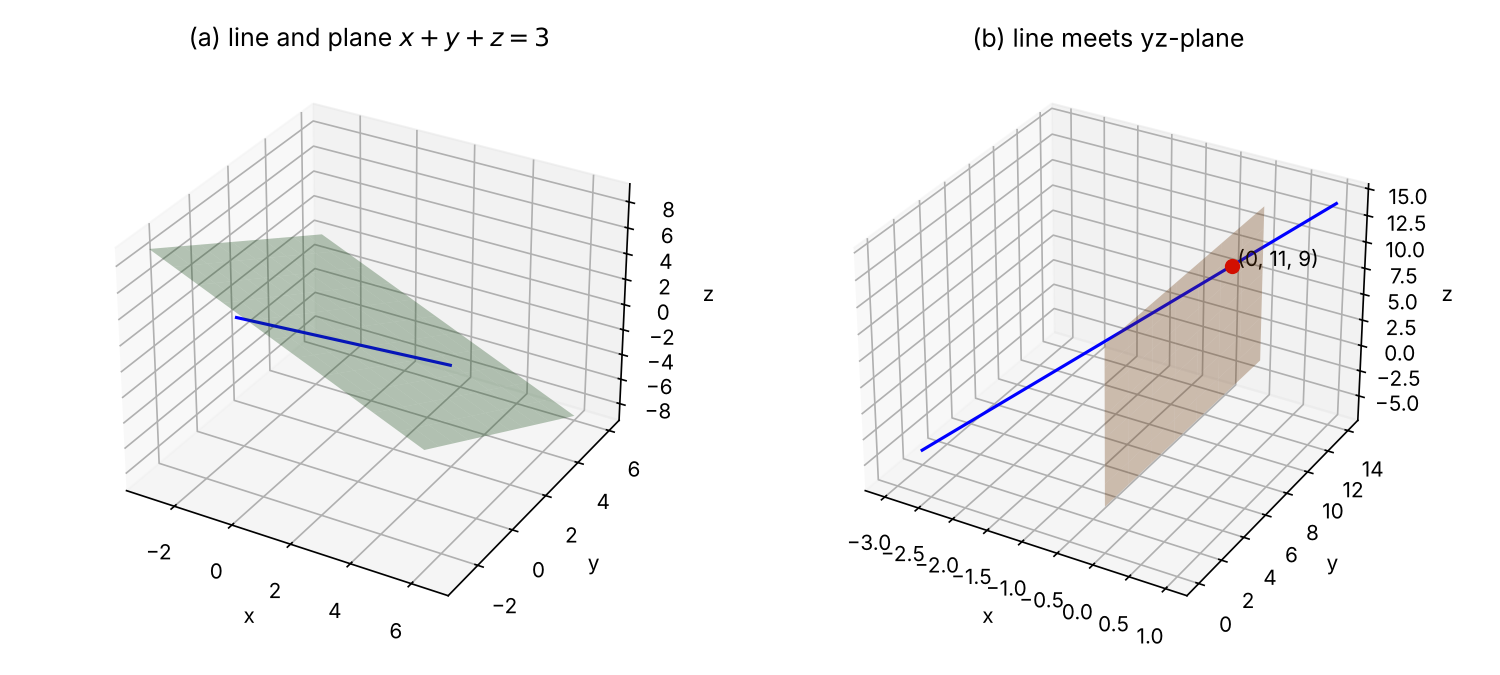
\includegraphics[width=0.95\linewidth]{figs/2.2.2.png}
    \caption{(a) Line and plane $x+y+z=3$; (b) line meeting the $yz$-plane at $(0,11,9)$}
    \label{fig:lineplane_q2}
\end{figure}

    \item Find the differential equation representing the family of curves $y = -A\cos 3x + B\sin 3x$.

\solution The family has two arbitrary constants $A$ and $B$, so by \ref{eq:EE26BTECH11225-family} we differentiate twice:
\begin{align}
    \frac{dy}{dx} &= 3A\sin 3x + 3B\cos 3x \\
    \frac{d^2y}{dx^2} &= 9A\cos 3x - 9B\sin 3x = -9\left(-A\cos 3x + B\sin 3x\right) = -9y
\end{align}
Hence the differential equation is
\begin{align}
    \frac{d^2y}{dx^2} + 9y = 0
\end{align}
The following code verifies this symbolically and plots members of the family in \figref{fig:odefamily_q3}.
\begin{lstlisting}[frame=single, basicstyle=\rmfamily, escapeinside={(*@}{@*)}]
(*@\makebox[\dimexpr\linewidth-2\fboxsep-2\fboxrule\relax][c]{codes/2.2.3.py}@*)
\end{lstlisting}
\begin{figure}[H]
    \centering
    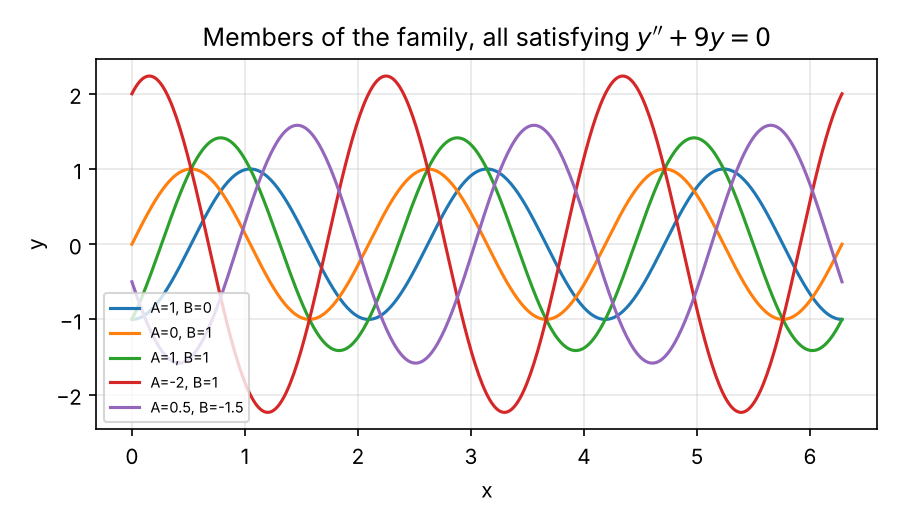
\includegraphics[width=0.75\linewidth]{figs/2.2.3.png}
    \caption{Members of the family $y=-A\cos 3x+B\sin 3x$}
    \label{fig:odefamily_q3}
\end{figure}

    \item Find the differential of the function $\cos^{-1}(\sin 2x)$ w.r.t. $x$.

\solution Since $\sin 2x = \cos\left(\frac{\pi}{2} - 2x\right)$, from \eqref{eq:EE26BTECH11225-invtrig-1}, for $\frac{\pi}{2}-2x \in [0,\pi]$, i.e. $-\frac{\pi}{4}\leq x\leq\frac{\pi}{4}$:
\begin{align}
    y &= \cos^{-1}\left(\cos\left(\frac{\pi}{2}-2x\right)\right) = \frac{\pi}{2} - 2x \\
    &\implies \frac{dy}{dx} = -2
\end{align}
The following code verifies the derivative numerically and plots \figref{fig:invtrig_q4}.
\begin{lstlisting}[frame=single, basicstyle=\rmfamily, escapeinside={(*@}{@*)}]
(*@\makebox[\dimexpr\linewidth-2\fboxsep-2\fboxrule\relax][c]{codes/2.2.4.py}@*)
\end{lstlisting}
\begin{figure}[H]
    \centering
    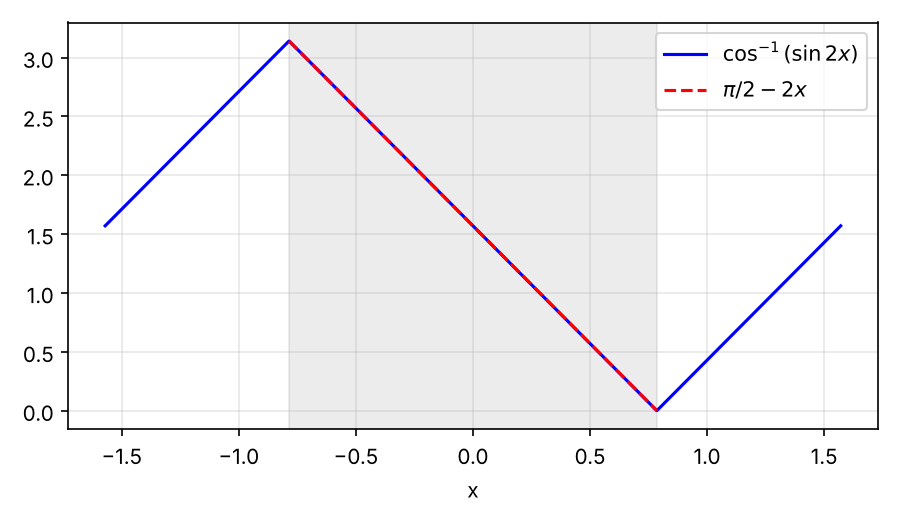
\includegraphics[width=0.70\linewidth]{figs/2.2.4.png}
    \caption{Plot of $\cos^{-1}(\sin 2x)$; it is the line $\frac{\pi}{2}-2x$ on the shaded region}
    \label{fig:invtrig_q4}
\end{figure}

    \item If an operation $*$ on the set of integers $\mathbb{Z}$ is defined by $a * b = 2a^2 + b$, then find (i) whether it is a binary or not, and (ii) if a binary, then is it commutative or not.

\solution (i) For any $a, b\in\mathbb{Z}$, $2a^2+b\in\mathbb{Z}$, so $*$ maps $\mathbb{Z}\times\mathbb{Z}\to\mathbb{Z}$ and is a binary operation. \\[4pt]
(ii) From \eqref{eq:EE26BTECH11225-binop}:
\begin{align}
    a * b = 2a^2 + b, \quad b * a = 2b^2 + a
\end{align}
For $a=1$, $b=2$:
\begin{align}
    1 * 2 = 2(1)^2 + 2 = 4, \quad 2 * 1 = 2(2)^2 + 1 = 9 \implies 1*2 \neq 2*1
\end{align}
Hence $*$ is a binary operation but it is not commutative.

    \item
    \begin{enumerate}[label=(\alph*), leftmargin=1.5em, labelsep=0.5em]
        \item Four cards are drawn one by one with replacement from a well-shuffled deck of playing cards. Find the probability that at least three cards are of diamonds.

        \begin{center}
            \textbf{OR}
        \end{center}

        \item The probability of two students $A$ and $B$ coming to school on time are $\frac{2}{7}$ and $\frac{4}{7}$, respectively. Assuming that the events `$A$ coming on time' and `$B$ coming on time' are independent, find the probability of only one of them coming to school on time.
    \end{enumerate} \vspace{2pt}
    \textbf{(a) Solution:} Let $X$ be the number of diamonds in $4$ draws with replacement. Then $X$ is binomial with $n=4$, $p=\frac{1}{4}$, and its PMF from \eqref{eq:EE26BTECH11225-pmf} is
\begin{align}
    p_X(k) = \binom{4}{k}\left(\frac{1}{4}\right)^k\left(\frac{3}{4}\right)^{4-k}, \quad k = 0,1,\dots,4
\end{align}
\begin{align}
    \Pr\brak{X\geq 3} = p_X(3) + p_X(4) = \frac{12}{256} + \frac{1}{256} = \frac{13}{256}
\end{align}
\textbf{(b) Solution:} Let $A, B \in \{0,1\}$ indicate that each student is on time, with $p_A(1)=\frac{2}{7}$ and $p_B(1)=\frac{4}{7}$. By independence, from \eqref{eq:EE26BTECH11225-pmf-joint}, $p_{AB}(a,b) = p_A(a)p_B(b)$, so
\begin{align}
    p_{AB}(1,0) = \frac{2}{7}\cdot\frac{3}{7} = \frac{6}{49}, \quad p_{AB}(0,1) = \frac{5}{7}\cdot\frac{4}{7} = \frac{20}{49}
\end{align}
\begin{align}
    \Pr\brak{\text{only one}} = p_{AB}(1,0) + p_{AB}(0,1) = \frac{26}{49}
\end{align}
The following code verifies both parts (exact fractions and a simulation) and plots \figref{fig:cards_q6}.
\begin{lstlisting}[frame=single, basicstyle=\rmfamily, escapeinside={(*@}{@*)}]
(*@\makebox[\dimexpr\linewidth-2\fboxsep-2\fboxrule\relax][c]{codes/2.2.6.py}@*)
\end{lstlisting}
\begin{figure}[H]
    \centering
    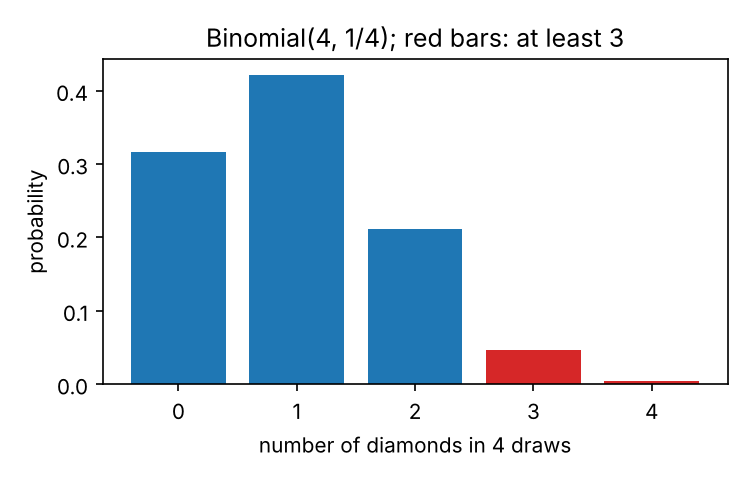
\includegraphics[width=0.55\linewidth]{figs/2.2.6.png}
    \caption{Distribution of the number of diamonds in four draws}
    \label{fig:cards_q6}
\end{figure}

    \item Find the value of $(x-y)$ from the matrix equation
\begin{align*}
    2\begin{bmatrix} x & 5 \\ 7 & y-3 \end{bmatrix} + \begin{bmatrix} -3 & -4 \\ 1 & 2 \end{bmatrix} = \begin{bmatrix} 7 & 6 \\ 15 & 14 \end{bmatrix}.
\end{align*}

\solution Moving the constant matrix to the right and dividing by $2$,
\begin{align}
    2\begin{bmatrix} x & 5 \\ 7 & y-3 \end{bmatrix} &= \begin{bmatrix} 7 & 6 \\ 15 & 14 \end{bmatrix} - \begin{bmatrix} -3 & -4 \\ 1 & 2 \end{bmatrix} = \begin{bmatrix} 10 & 10 \\ 14 & 12 \end{bmatrix} \\
    \begin{bmatrix} x & 5 \\ 7 & y-3 \end{bmatrix} &= \begin{bmatrix} 5 & 5 \\ 7 & 6 \end{bmatrix}
\end{align}
Comparing entries, $x = 5$ and $y - 3 = 6 \implies y = 9$. Hence
\begin{align}
    x - y = 5 - 9 = -4
\end{align}

    \item Solve the following differential equation:
\begin{align*}
    (y + 3x^2)\frac{dx}{dy} = x
\end{align*}

\solution Taking reciprocals, $\frac{dy}{dx} = \frac{y+3x^2}{x}$, that is,
\begin{align}
    x y' - y = 3x^2
\end{align}
The equation is singular at $x=0$, so we look for solutions with $y(0)=0$ and let $y'(0)=C$. With $Y(s) = \mathcal{L}\{y\}$, \eqref{eq:EE26BTECH11225-laplace-deriv} gives $\mathcal{L}\{y'\} = sY$ and so $\mathcal{L}\{xy'\} = -\frac{d}{ds}(sY) = -sY'-Y$. Using $\mathcal{L}\{3x^2\} = \frac{6}{s^3}$ from \eqref{eq:EE26BTECH11225-laplace},
\begin{align}
    -sY' - Y - Y &= \frac{6}{s^3} \\
    \implies s^2Y' + 2sY = \brak{s^2Y}' &= -\frac{6}{s^2}
\end{align}
Integrating, $s^2Y = \frac{6}{s} + C$, so
\begin{align}
    Y(s) = \frac{6}{s^3} + \frac{C}{s^2} \implies y = 3x^2 + Cx
\end{align}
The following code verifies the solution and plots \figref{fig:linearode_q8}.
\begin{lstlisting}[frame=single, basicstyle=\rmfamily, escapeinside={(*@}{@*)}]
(*@\makebox[\dimexpr\linewidth-2\fboxsep-2\fboxrule\relax][c]{codes/2.2.8.py}@*)
\end{lstlisting}
\begin{figure}[H]
    \centering
    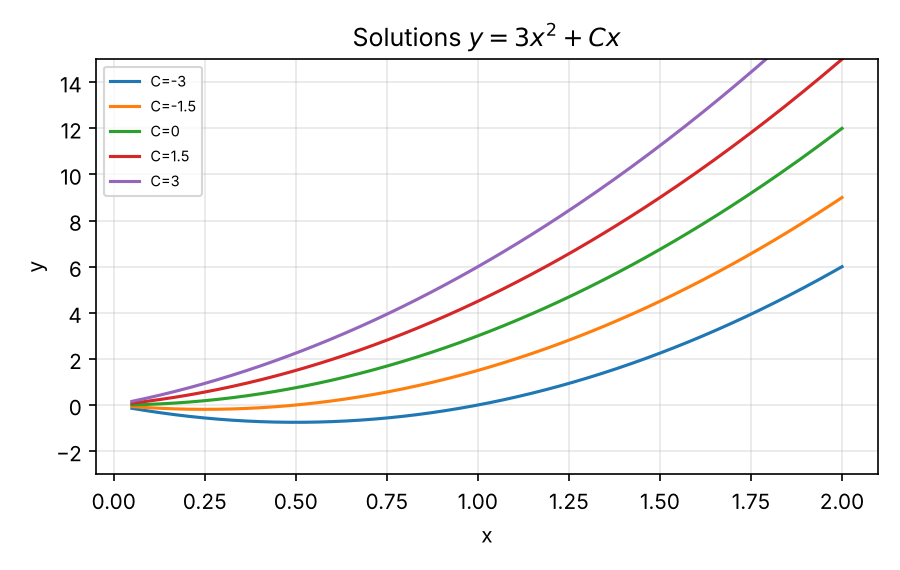
\includegraphics[width=0.70\linewidth]{figs/2.2.8.png}
    \caption{Solutions $y=3x^2+Cx$ for several values of $C$}
    \label{fig:linearode_q8}
\end{figure}

    \item
    \begin{enumerate}[label=(\alph*), leftmargin=1.5em, labelsep=0.5em]
        \item Using vectors, prove that the points $(2,-1,3)$, $(3,-5,1)$ and $(-1,11,9)$ are collinear.

        \begin{center}
            \textbf{OR}
        \end{center}

        \item For any two vectors $\vec{a}$ and $\vec{b}$, prove that $(\vec{a}\times\vec{b})^2 = \vec{a}^2\vec{b}^2 - (\vec{a}\cdot\vec{b})^2$.
    \end{enumerate} \vspace{2pt}
    \textbf{(a) Solution:} Let $A(2,-1,3)$, $B(3,-5,1)$, $C(-1,11,9)$.
\begin{align}
    \vec{AB} &= \myvec{3-2 \\ -5+1 \\ 1-3} = \myvec{1 \\ -4 \\ -2} \\
    \vec{BC} &= \myvec{-1-3 \\ 11+5 \\ 9-1} = \myvec{-4 \\ 16 \\ 8} = -4\myvec{1 \\ -4 \\ -2} = -4\,\vec{AB}
\end{align}
Since $\vec{BC} = k\,\vec{AB}$ with $k=-4$ and $B$ is common to both, the points $A$, $B$, $C$ are collinear. \\[8pt]
\textbf{(b) Solution:} Let $\theta$ be the angle between $\vec{a}$ and $\vec{b}$. From \eqref{eq:EE26BTECH11225-cross},
\begin{align}
    \|\vec{a}\times\vec{b}\|^2 &= \|\vec{a}\|^2\|\vec{b}\|^2\sin^2\theta \\
    &= \|\vec{a}\|^2\|\vec{b}\|^2\left(1-\cos^2\theta\right) \\
    &= \|\vec{a}\|^2\|\vec{b}\|^2 - \left(\|\vec{a}\|\|\vec{b}\|\cos\theta\right)^2
\end{align}
and, from \eqref{eq:EE26BTECH11225-dot}, $\|\vec{a}\|\|\vec{b}\|\cos\theta = \vec{a}^{\top}\vec{b}$. Hence
\begin{align}
    \|\vec{a}\times\vec{b}\|^2 = \|\vec{a}\|^2\|\vec{b}\|^2 - \left(\vec{a}^{\top}\vec{b}\right)^2
\end{align}
The following code verifies both parts and generates \figref{fig:collinear_q9}.
\begin{lstlisting}[frame=single, basicstyle=\rmfamily, escapeinside={(*@}{@*)}]
(*@\makebox[\dimexpr\linewidth-2\fboxsep-2\fboxrule\relax][c]{codes/2.2.9.py}@*)
\end{lstlisting}
\begin{figure}[H]
    \centering
    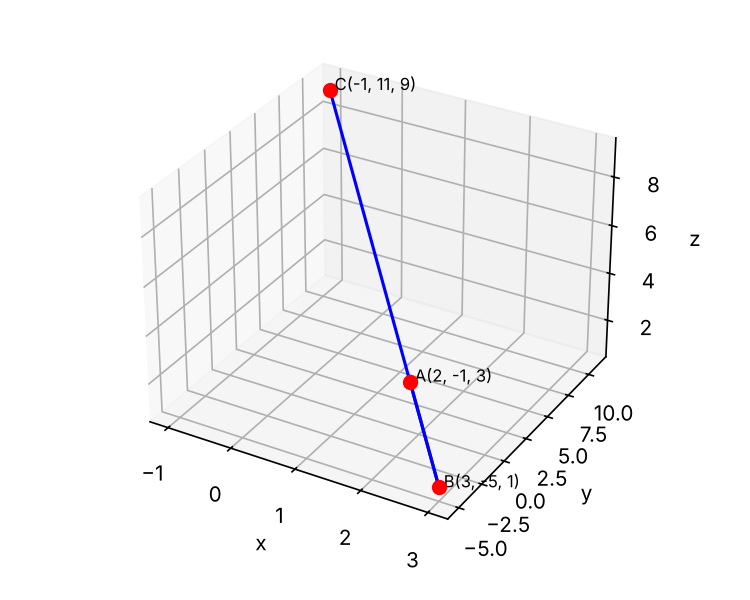
\includegraphics[width=0.55\linewidth]{figs/2.2.9.png}
    \caption{The collinear points $A$, $B$, $C$}
    \label{fig:collinear_q9}
\end{figure}

    \item
    \begin{enumerate}[label=(\alph*), leftmargin=1.5em, labelsep=0.5em]
        \item Find: $\displaystyle\int\frac{x-1}{(x-2)(x-3)}\,dx$

        \begin{center}
            \textbf{OR}
        \end{center}

        \item Integrate: $\dfrac{e^x}{\sqrt{5-4e^x-e^{2x}}}$ with respect to $x$.
    \end{enumerate} \vspace{2pt}
    \textbf{(a) Solution:} Using partial fractions, $\frac{x-1}{(x-2)(x-3)} = \frac{A}{x-2}+\frac{B}{x-3}$:
\begin{align}
    A = \frac{2-1}{2-3} = -1, \quad B = \frac{3-1}{3-2} = 2
\end{align}
\begin{align}
    \int\frac{x-1}{(x-2)(x-3)}dx &= -\int\frac{dx}{x-2} + 2\int\frac{dx}{x-3} \\
    &= -\ln|x-2| + 2\ln|x-3| + C
\end{align}
\textbf{(b) Solution:} Let $t = e^x$, so $dt = e^x dx$. Since $5-4t-t^2 = 9-(t+2)^2$, from \eqref{eq:EE26BTECH11225-sininv}:
\begin{align}
    \int\frac{dt}{\sqrt{5-4t-t^2}} &= \int\frac{dt}{\sqrt{9-(t+2)^2}} \\
    &= \sin^{-1}\left(\frac{t+2}{3}\right) + C = \sin^{-1}\left(\frac{e^x+2}{3}\right) + C
\end{align}
(The integrand is real only for $e^x<1$, i.e. $x<0$.) The following code verifies both antiderivatives by differentiation.
\begin{lstlisting}[frame=single, basicstyle=\rmfamily, escapeinside={(*@}{@*)}]
(*@\makebox[\dimexpr\linewidth-2\fboxsep-2\fboxrule\relax][c]{codes/2.2.10.py}@*)
\end{lstlisting}

    \item Find: $\displaystyle\int e^x\left(\frac{2+\sin 2x}{2\cos^2 x}\right)dx$

\solution Using $\sin 2x = 2\sin x\cos x$:
\begin{align}
    \frac{2+\sin 2x}{2\cos^2 x} = \frac{1}{\cos^2 x} + \frac{2\sin x\cos x}{2\cos^2 x} = \sec^2 x + \tan x
\end{align}
With $f(x) = \tan x$ and $f'(x) = \sec^2 x$, from \eqref{eq:EE26BTECH11225-expint}:
\begin{align}
    \int e^x(\tan x+\sec^2 x)\,dx = e^x\tan x + C
\end{align}
The following code verifies the result by differentiation.
\begin{lstlisting}[frame=single, basicstyle=\rmfamily, escapeinside={(*@}{@*)}]
(*@\makebox[\dimexpr\linewidth-2\fboxsep-2\fboxrule\relax][c]{codes/2.2.11.py}@*)
\end{lstlisting}

    \item If $A$ and $B$ are independent events with $P(A) = \frac{3}{7}$ and $P(B) = \frac{2}{5}$, then find $P(A'\cap B')$.

\solution Let $A, B \in \{0,1\}$ be the indicators of the two events, with $p_A(1) = \frac{3}{7}$ and $p_B(1) = \frac{2}{5}$. By independence, from \eqref{eq:EE26BTECH11225-pmf-joint}, $p_{AB}(a,b) = p_A(a)p_B(b)$. Neither event occurs when $(A,B) = (0,0)$:
\begin{align}
    p_{AB}(0,0) = \frac{4}{7}\cdot\frac{3}{5} = \frac{12}{35}
\end{align}
Hence $P(A'\cap B') = \frac{12}{35}$.

    \item Find the equation of the plane passing through the point $(-1,3,2)$ and perpendicular to the planes $x+2y+3z=5$ and $3x+3y+z=0$.

\solution The normals of the given planes are $\vec{n}_1 = \myvec{1\\2\\3}$ and $\vec{n}_2 = \myvec{3\\3\\1}$. From \eqref{eq:EE26BTECH11225-plane},
\begin{align}
    \vec{n} = \vec{n}_1\times\vec{n}_2 = \myvec{2\cdot1-3\cdot3 \\ 3\cdot3-1\cdot1 \\ 1\cdot3-2\cdot3} = \myvec{-7 \\ 8 \\ -3}
\end{align}
The plane through $\vec{P}_0 = \myvec{-1\\3\\2}$ is $\vec{n}^{\top}(\vec{x}-\vec{P}_0) = 0$:
\begin{align}
    -7(x+1) + 8(y-3) - 3(z-2) &= 0 \\
    \implies -7x + 8y - 3z - 25 &= 0 \\
    \implies 7x - 8y + 3z + 25 &= 0
\end{align}
The following code verifies $\vec{n}\perp\vec{n}_1,\vec{n}_2$ and plots \figref{fig:plane_q13}.
\begin{lstlisting}[frame=single, basicstyle=\rmfamily, escapeinside={(*@}{@*)}]
(*@\makebox[\dimexpr\linewidth-2\fboxsep-2\fboxrule\relax][c]{codes/2.2.13.py}@*)
\end{lstlisting}
\begin{figure}[H]
    \centering
    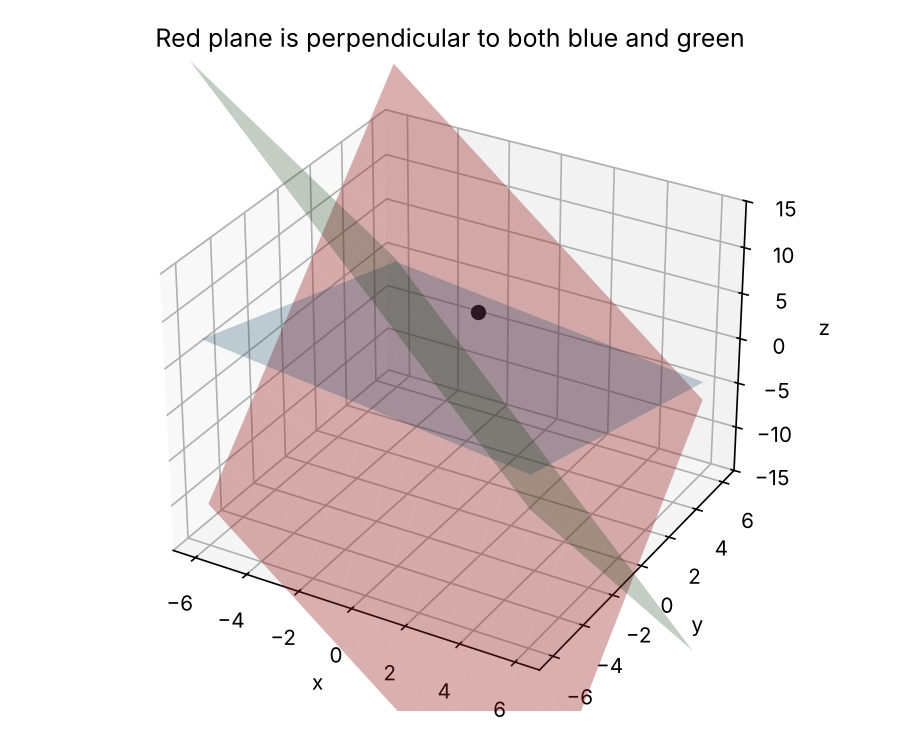
\includegraphics[width=0.65\linewidth]{figs/2.2.13.png}
    \caption{The required plane (red) with the two given planes}
    \label{fig:plane_q13}
\end{figure}

    \item Evaluate: $\displaystyle\int_1^5 \big(|x-1| + |x-2| + |x-4|\big)\,dx$

\solution Write each term with the unit step, $|x-a| = (a-x) + 2(x-a)u(x-a)$, from \eqref{eq:EE26BTECH11225-laplace-step}. For $x \ge 0$,
\begin{align}
    f(x) = 7 - 3x + 2\left[(x-1)u(x-1) + (x-2)u(x-2) + (x-4)u(x-4)\right]
\end{align}
Its transform from \eqref{eq:EE26BTECH11225-laplace} and \eqref{eq:EE26BTECH11225-laplace-step} is
\begin{align}
    F(s) = \frac{7}{s} - \frac{3}{s^2} + \frac{2}{s^2}\left(e^{-s}+e^{-2s}+e^{-4s}\right)
\end{align}
Dividing by $s$ as in \eqref{eq:EE26BTECH11225-laplace-int} gives $G(s) = \frac{F(s)}{s}$, and inverting, the integral $g(x) = \int_0^x f$ is
\begin{align}
    g(x) = 7x - \frac{3x^2}{2} + (x-1)^2u(x-1) + (x-2)^2u(x-2) + (x-4)^2u(x-4)
\end{align}
\begin{align}
    \int_1^5 f(x)\,dx = g(5) - g(1) = \left(35 - \frac{75}{2} + 16 + 9 + 1\right) - \left(7 - \frac{3}{2}\right) = \frac{47}{2} - \frac{11}{2} = 18
\end{align}
The following code verifies the Laplace result and plots \figref{fig:absint_q14}.
\begin{lstlisting}[frame=single, basicstyle=\rmfamily, escapeinside={(*@}{@*)}]
(*@\makebox[\dimexpr\linewidth-2\fboxsep-2\fboxrule\relax][c]{codes/2.2.14.py}@*)
\end{lstlisting}
\begin{figure}[H]
    \centering
    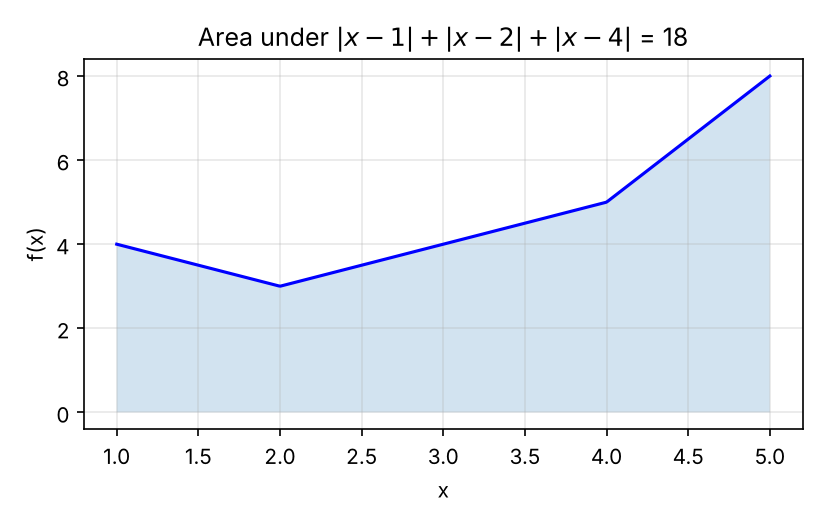
\includegraphics[width=0.60\linewidth]{figs/2.2.14.png}
    \caption{Area under $|x-1|+|x-2|+|x-4|$ from $x=1$ to $x=5$}
    \label{fig:absint_q14}
\end{figure}

    \item If $x,y,z$ are different and $\Delta = \begin{vmatrix} x & x^2 & x^3-1 \\ y & y^2 & y^3-1 \\ z & z^2 & z^3-1 \end{vmatrix} = 0$, then using properties of determinants, show that $xyz=1$.

\solution Splitting the third column:
\begin{align}
    \Delta &= \begin{vmatrix} x & x^2 & x^3 \\ y & y^2 & y^3 \\ z & z^2 & z^3 \end{vmatrix} - \begin{vmatrix} x & x^2 & 1 \\ y & y^2 & 1 \\ z & z^2 & 1 \end{vmatrix}
\end{align}
Taking $x$, $y$, $z$ common from the rows of the first determinant, and moving the last column of the second determinant to the front (two column interchanges, so the sign is unchanged):
\begin{align}
    \Delta &= xyz\begin{vmatrix} 1 & x & x^2 \\ 1 & y & y^2 \\ 1 & z & z^2 \end{vmatrix} - \begin{vmatrix} 1 & x & x^2 \\ 1 & y & y^2 \\ 1 & z & z^2 \end{vmatrix} \\
    &= (xyz-1)\begin{vmatrix} 1 & x & x^2 \\ 1 & y & y^2 \\ 1 & z & z^2 \end{vmatrix} \\
    &= (xyz-1)(y-x)(z-x)(z-y) = 0
\end{align}
Since $x,y,z$ are different, $(y-x)(z-x)(z-y)\neq 0$. Hence $xyz - 1 = 0$, i.e. $xyz = 1$. The following code factorises $\Delta$ symbolically.
\begin{lstlisting}[frame=single, basicstyle=\rmfamily, escapeinside={(*@}{@*)}]
(*@\makebox[\dimexpr\linewidth-2\fboxsep-2\fboxrule\relax][c]{codes/2.2.15.py}@*)
\end{lstlisting}

    \item Prove that: $\sin^{-1}\dfrac{4}{5} + \tan^{-1}\dfrac{5}{12} + \cos^{-1}\dfrac{63}{65} = \dfrac{\pi}{2}$

\solution Write $\sin^{-1}\frac{4}{5}$ and $\cos^{-1}\frac{63}{65}$ in terms of $\tan^{-1}$ (from the right triangles with sides $3,4,5$ and $16,63,65$):
\begin{align}
    \sin^{-1}\frac{4}{5} = \tan^{-1}\frac{4}{3}, \quad \cos^{-1}\frac{63}{65} = \tan^{-1}\frac{16}{63}
\end{align}
From \eqref{eq:EE26BTECH11225-invtrig-2} (here $ab = \frac{4}{3}\cdot\frac{5}{12} = \frac{5}{9} < 1$):
\begin{align}
    \tan^{-1}\frac{4}{3}+\tan^{-1}\frac{5}{12} &= \tan^{-1}\frac{\frac{4}{3}+\frac{5}{12}}{1-\frac{20}{36}} = \tan^{-1}\frac{63}{16}
\end{align}
Since $\tan^{-1}\frac{16}{63} = \cot^{-1}\frac{63}{16}$, from \eqref{eq:EE26BTECH11225-invtrig-3}:
\begin{align}
    \text{LHS} = \tan^{-1}\frac{63}{16}+\cot^{-1}\frac{63}{16} = \frac{\pi}{2} = \text{RHS}
\end{align}
Hence proved. The following code verifies each step numerically.
\begin{lstlisting}[frame=single, basicstyle=\rmfamily, escapeinside={(*@}{@*)}]
(*@\makebox[\dimexpr\linewidth-2\fboxsep-2\fboxrule\relax][c]{codes/2.2.16.py}@*)
\end{lstlisting}

    \item Using vectors, find the value of $x$ such that the four points $A(x,5,-1)$, $B(3,2,1)$, $C(4,5,5)$ and $D(4,2,-2)$ are coplanar.

\solution From \eqref{eq:EE26BTECH11225-coplanar}, the points are coplanar if $\det\begin{bmatrix}\vec{AB} & \vec{AC} & \vec{AD}\end{bmatrix}=0$. Here
\begin{align}
    \vec{AB} = \myvec{3-x \\ -3 \\ 2}, \quad \vec{AC} = \myvec{4-x \\ 0 \\ 6}, \quad \vec{AD} = \myvec{4-x \\ -3 \\ -1}
\end{align}
\begin{align}
    \begin{vmatrix} 3-x & 4-x & 4-x \\ -3 & 0 & -3 \\ 2 & 6 & -1 \end{vmatrix} &= 0 \\
    (3-x)\big[0+18\big] - (4-x)\big[3+6\big] + (4-x)\big[-18-0\big] &= 0 \\
    18(3-x) - 9(4-x) - 18(4-x) &= 0 \\
    54 - 18x - 27(4-x) &= 0 \\
    9x - 54 &= 0 \implies x = 6
\end{align}
The following code solves for $x$, checks that the determinant vanishes at $x=6$ and plots \figref{fig:coplanar_q17}.
\begin{lstlisting}[frame=single, basicstyle=\rmfamily, escapeinside={(*@}{@*)}]
(*@\makebox[\dimexpr\linewidth-2\fboxsep-2\fboxrule\relax][c]{codes/2.2.17.py}@*)
\end{lstlisting}
\begin{figure}[H]
    \centering
    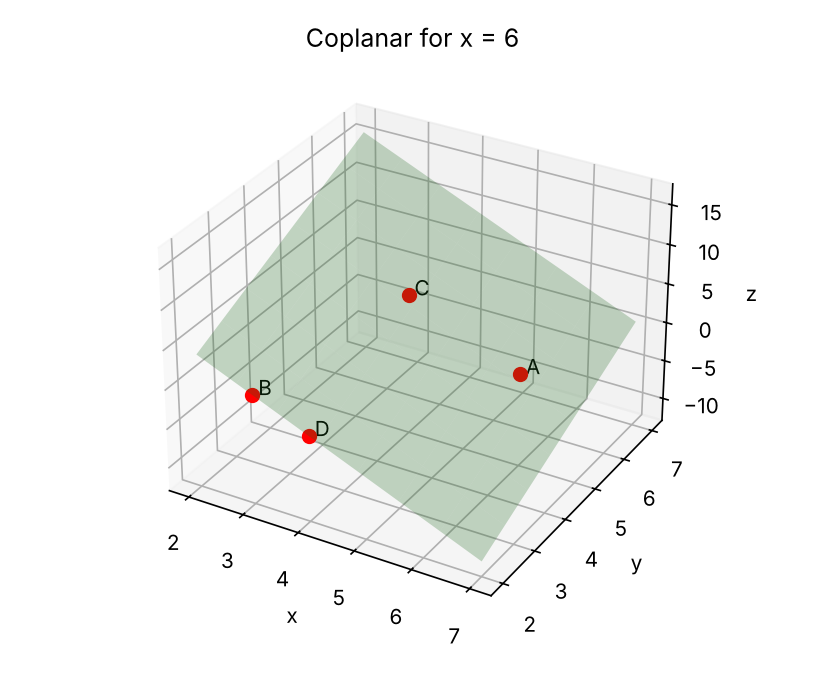
\includegraphics[width=0.60\linewidth]{figs/2.2.17.png}
    \caption{The four coplanar points for $x=6$}
    \label{fig:coplanar_q17}
\end{figure}

    \item
    \begin{enumerate}[label=(\alph*), leftmargin=1.5em, labelsep=0.5em]
        \item Differentiate $\tan^{-1}\dfrac{3x-x^3}{1-3x^2}$, $|x|<\dfrac{1}{\sqrt{3}}$ w.r.t. $\tan^{-1}\dfrac{x}{\sqrt{1-x^2}}$.

        \begin{center}
            \textbf{OR}
        \end{center}

        \item If $\sqrt{1-x^2}+\sqrt{1-y^2} = a(x-y)$, $|x|<1$, $|y|<1$, show that $\dfrac{dy}{dx} = \sqrt{\dfrac{1-y^2}{1-x^2}}$.
    \end{enumerate} \vspace{2pt}
    \textbf{(a) Solution:} Let $u = \tan^{-1}\frac{3x-x^3}{1-3x^2}$ and $v = \tan^{-1}\frac{x}{\sqrt{1-x^2}}$. Put $x=\tan\phi$; since $|x|<\frac{1}{\sqrt{3}}$, $|3\phi|<\frac{\pi}{2}$ and
\begin{align}
    u = \tan^{-1}(\tan 3\phi) = 3\phi = 3\tan^{-1}x \implies \frac{du}{dx} = \frac{3}{1+x^2}
\end{align}
From \eqref{eq:EE26BTECH11225-invtrig-4}, $v = \sin^{-1}x$, so $\frac{dv}{dx} = \frac{1}{\sqrt{1-x^2}}$. Hence
\begin{align}
    \frac{du}{dv} = \frac{du/dx}{dv/dx} = \frac{3\sqrt{1-x^2}}{1+x^2}
\end{align}
\textbf{(b) Solution:} Put $x=\sin\alpha$, $y=\sin\beta$ with $\alpha,\beta\in\left(-\frac{\pi}{2},\frac{\pi}{2}\right)$:
\begin{align}
    \cos\alpha + \cos\beta &= a(\sin\alpha - \sin\beta) \\
    2\cos\frac{\alpha+\beta}{2}\cos\frac{\alpha-\beta}{2} &= 2a\cos\frac{\alpha+\beta}{2}\sin\frac{\alpha-\beta}{2} \\
    \implies \cot\frac{\alpha-\beta}{2} = a &\implies \sin^{-1}x - \sin^{-1}y = 2\cot^{-1}a
\end{align}
Differentiating w.r.t. $x$ (the right side is a constant):
\begin{align}
    \frac{1}{\sqrt{1-x^2}} - \frac{1}{\sqrt{1-y^2}}\frac{dy}{dx} = 0 \implies \frac{dy}{dx} = \sqrt{\frac{1-y^2}{1-x^2}}
\end{align}
The following code verifies both parts and plots \figref{fig:diff_q18}.
\begin{lstlisting}[frame=single, basicstyle=\rmfamily, escapeinside={(*@}{@*)}]
(*@\makebox[\dimexpr\linewidth-2\fboxsep-2\fboxrule\relax][c]{codes/2.2.18.py}@*)
\end{lstlisting}
\begin{figure}[H]
    \centering
    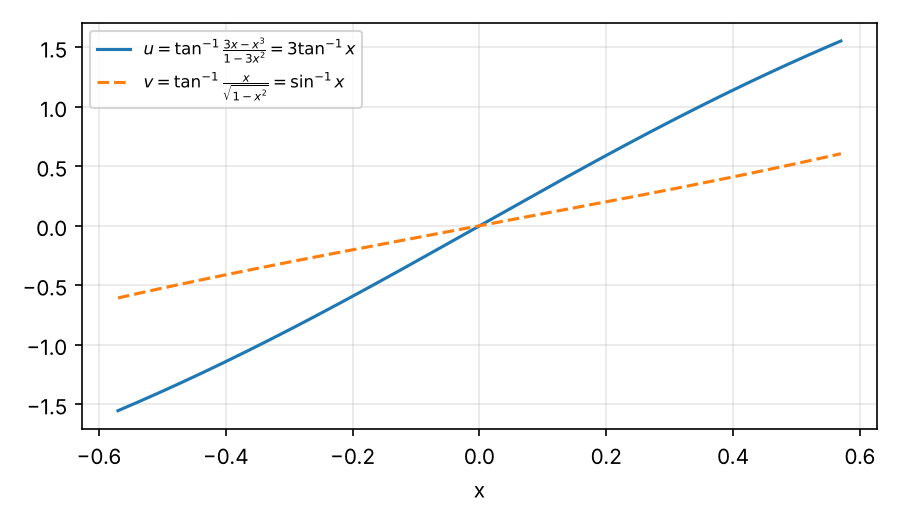
\includegraphics[width=0.65\linewidth]{figs/2.2.18.png}
    \caption{The functions $u=3\tan^{-1}x$ and $v=\sin^{-1}x$}
    \label{fig:diff_q18}
\end{figure}

    \item
    \begin{enumerate}[label=(\alph*), leftmargin=1.5em, labelsep=0.5em]
        \item Prove that the relation $R$ in the set $A = \{1,2,3,4,5,6,7\}$ given by $R = \{(a,b) : |a-b| \text{ is even}\}$ is an equivalence relation.

        \begin{center}
            \textbf{OR}
        \end{center}

        \item Show that the function $f$ in $A = \mathbb{R}-\left\{\frac{2}{3}\right\}$ defined as $f(x) = \dfrac{4x+3}{6x-4}$ is one-one and onto. Hence, find $f^{-1}$.
    \end{enumerate} \vspace{2pt}
    \textbf{(a) Solution:} By \ref{eq:EE26BTECH11225-equiv} we check three properties.
\begin{align}
    \text{Reflexive: } & |a-a| = 0 \text{ is even} \implies (a,a)\in R \\
    \text{Symmetric: } & |a-b| = |b-a| \implies (a,b)\in R \Rightarrow (b,a)\in R \\
    \text{Transitive: } & |a-b|,\,|b-c| \text{ even} \implies a-c = (a-b)+(b-c) \text{ is even}
\end{align}
Hence $R$ is an equivalence relation. \\[8pt]
\textbf{(b) Solution:} \emph{One-one:} Let $f(x_1) = f(x_2)$:
\begin{align}
    (4x_1+3)(6x_2-4) &= (4x_2+3)(6x_1-4) \\
    24x_1x_2 - 16x_1 + 18x_2 - 12 &= 24x_1x_2 - 16x_2 + 18x_1 - 12 \\
    34x_2 = 34x_1 &\implies x_1 = x_2
\end{align}
\emph{Onto:} Let $y = \frac{4x+3}{6x-4}$, $y \neq \frac{2}{3}$. Solving for $x$:
\begin{align}
    6xy - 4y = 4x+3 \implies x = \frac{4y+3}{6y-4}
\end{align}
This $x$ is defined for every $y\neq\frac{2}{3}$, and $x\neq\frac{2}{3}$ (otherwise $12y+9=12y-8$, which is impossible). So every $y\in A$ has a pre-image and $f$ is onto. Hence
\begin{align}
    f^{-1}(y) = \frac{4y+3}{6y-4}, \quad \text{i.e. } f^{-1} = f
\end{align}
The following code verifies both parts and generates \figref{fig:equiv_q19}.
\begin{lstlisting}[frame=single, basicstyle=\rmfamily, escapeinside={(*@}{@*)}]
(*@\makebox[\dimexpr\linewidth-2\fboxsep-2\fboxrule\relax][c]{codes/2.2.19.py}@*)
\end{lstlisting}
\begin{figure}[H]
    \centering
    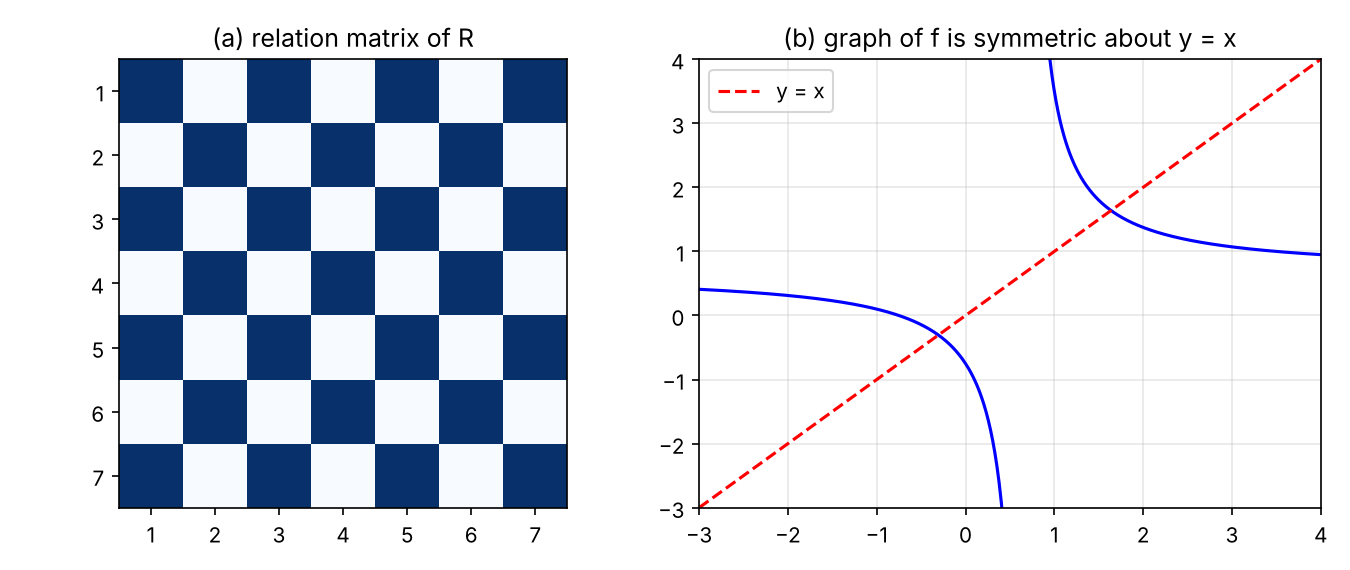
\includegraphics[width=0.95\linewidth]{figs/2.2.19.png}
    \caption{(a) Relation matrix of $R$; (b) graph of $f$, symmetric about $y=x$}
    \label{fig:equiv_q19}
\end{figure}

    \item
    \begin{enumerate}[label=(\alph*), leftmargin=1.5em, labelsep=0.5em]
        \item Find the particular solution of the differential equation $(1+e^{2x})\,dy + (1+y^2)e^x\,dx = 0$, given that $y(0)=1$.

        \begin{center}
            \textbf{OR}
        \end{center}

        \item Find the particular solution of the differential equation $x\dfrac{dy}{dx}\sin\left(\dfrac{y}{x}\right) + x - y\sin\left(\dfrac{y}{x}\right) = 0$, given that $y(1) = \dfrac{\pi}{2}$.
    \end{enumerate} \vspace{2pt}
    \textbf{(a) Solution:} Separating the variables:
\begin{align}
    \frac{dy}{1+y^2} &= -\frac{e^x\,dx}{1+e^{2x}} \\
    \tan^{-1}y &= -\tan^{-1}(e^x) + C
\end{align}
Using $y(0)=1$: $\frac{\pi}{4} = -\frac{\pi}{4}+C \implies C = \frac{\pi}{2}$. Then from \eqref{eq:EE26BTECH11225-invtrig-3},
\begin{align}
    \tan^{-1}y = \frac{\pi}{2}-\tan^{-1}(e^x) = \cot^{-1}(e^x) = \tan^{-1}(e^{-x}) \implies y = e^{-x}
\end{align}
\textbf{(b) Solution:} Dividing by $x\sin\left(\frac{y}{x}\right)$:
\begin{align}
    \frac{dy}{dx} = \frac{y}{x} - \frac{1}{\sin(y/x)}
\end{align}
This is homogeneous. From \eqref{eq:EE26BTECH11225-homog}, put $y=vx$:
\begin{align}
    v + x\frac{dv}{dx} &= v - \frac{1}{\sin v} \\
    \sin v\,dv &= -\frac{dx}{x} \\
    -\cos v &= -\ln|x| + C \implies \cos\left(\frac{y}{x}\right) = \ln|x| + C'
\end{align}
Using $y(1)=\frac{\pi}{2}$: $\cos\frac{\pi}{2} = 0 = \ln 1 + C' \implies C'=0$. Hence
\begin{align}
    \cos\left(\frac{y}{x}\right) = \ln|x|
\end{align}
The following code verifies both solutions and plots \figref{fig:solveode_q20}.
\begin{lstlisting}[frame=single, basicstyle=\rmfamily, escapeinside={(*@}{@*)}]
(*@\makebox[\dimexpr\linewidth-2\fboxsep-2\fboxrule\relax][c]{codes/2.2.20.py}@*)
\end{lstlisting}
\begin{figure}[H]
    \centering
    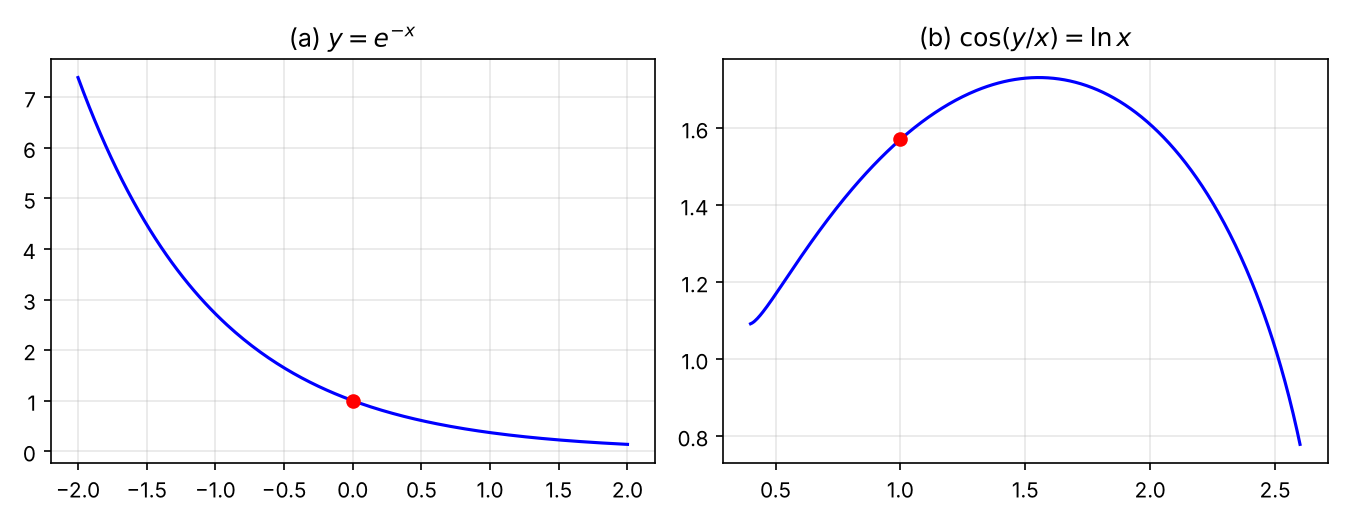
\includegraphics[width=0.95\linewidth]{figs/2.2.20.png}
    \caption{(a) $y=e^{-x}$ and (b) $\cos(y/x)=\ln x$}
    \label{fig:solveode_q20}
\end{figure}

    \item If $y = (\sin x)^x + \sin^{-1}\left(\sqrt{1-x^2}\right)$, then find $\dfrac{dy}{dx}$.

\solution The function is defined for $0<x<1$ (we need $\sin x>0$ and $|x|\leq1$). Let $y = u + w$ with $u = (\sin x)^x$ and $w = \sin^{-1}\sqrt{1-x^2}$. From \eqref{eq:EE26BTECH11225-logdiff}:
\begin{align}
    \ln u = x\ln\sin x &\implies \frac{1}{u}\frac{du}{dx} = \ln\sin x + x\cot x \\
    &\implies \frac{du}{dx} = (\sin x)^x\left(x\cot x + \ln\sin x\right)
\end{align}
For $0<x<1$ put $x=\cos\phi$, $\phi\in\left(0,\frac{\pi}{2}\right)$; then $\sqrt{1-x^2}=\sin\phi$ and $w = \phi = \cos^{-1}x$:
\begin{align}
    \frac{dw}{dx} = -\frac{1}{\sqrt{1-x^2}}
\end{align}
Hence
\begin{align}
    \frac{dy}{dx} = (\sin x)^x\left(x\cot x+\ln\sin x\right) - \frac{1}{\sqrt{1-x^2}}
\end{align}
The following code verifies the derivative and plots \figref{fig:logdiff_q21}.
\begin{lstlisting}[frame=single, basicstyle=\rmfamily, escapeinside={(*@}{@*)}]
(*@\makebox[\dimexpr\linewidth-2\fboxsep-2\fboxrule\relax][c]{codes/2.2.21.py}@*)
\end{lstlisting}
\begin{figure}[H]
    \centering
    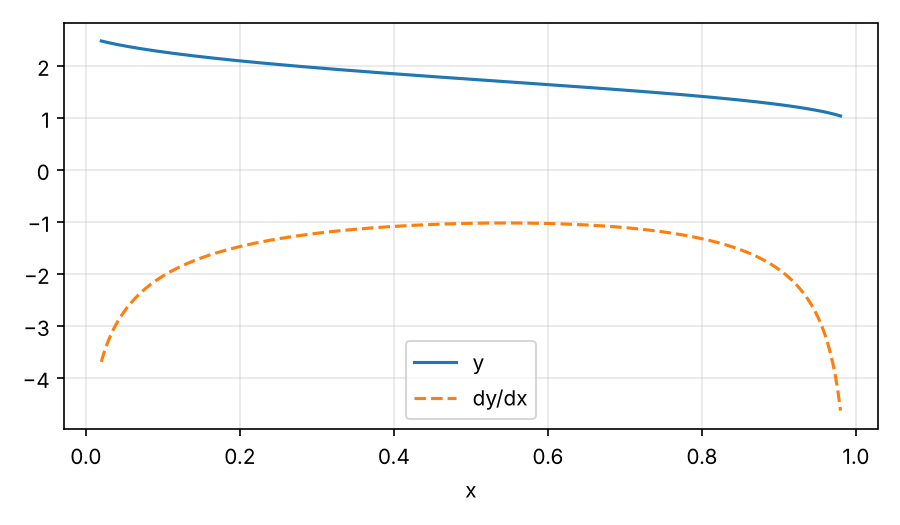
\includegraphics[width=0.65\linewidth]{figs/2.2.21.png}
    \caption{The function $y$ and its derivative on $(0,1)$}
    \label{fig:logdiff_q21}
\end{figure}

    \item Find: $\displaystyle\int\cos 2x\cos 4x\cos 6x\,dx$

\solution From \eqref{eq:EE26BTECH11225-prodsum}, the integrand is a sum of cosines:
\begin{align}
    f(x) = \cos 2x\cos 4x\cos 6x = \frac{1}{4}\left(1+\cos 12x+\cos 8x+\cos 4x\right)
\end{align}
Taking the Laplace transform with \eqref{eq:EE26BTECH11225-laplace},
\begin{align}
    F(s) = \frac{1}{4}\left[\frac{1}{s}+\frac{s}{s^2+144}+\frac{s}{s^2+64}+\frac{s}{s^2+16}\right]
\end{align}
Dividing by $s$ as in \eqref{eq:EE26BTECH11225-laplace-int} gives the transform of the integral:
\begin{align}
    G(s) = \frac{F(s)}{s} = \frac{1}{4}\left[\frac{1}{s^2}+\frac{1}{s^2+144}+\frac{1}{s^2+64}+\frac{1}{s^2+16}\right]
\end{align}
Using $\mathcal{L}^{-1}\left\{\frac{1}{s^2+\omega^2}\right\} = \frac{\sin\omega x}{\omega}$ and $\mathcal{L}^{-1}\left\{\frac{1}{s^2}\right\} = x$,
\begin{align}
    \int\cos 2x\cos 4x\cos 6x\,dx = \frac{1}{4}\left[x+\frac{\sin 12x}{12}+\frac{\sin 8x}{8}+\frac{\sin 4x}{4}\right] + C
\end{align}
The following code computes the Laplace transform and its inverse, and checks the result by differentiation.
\begin{lstlisting}[frame=single, basicstyle=\rmfamily, escapeinside={(*@}{@*)}]
(*@\makebox[\dimexpr\linewidth-2\fboxsep-2\fboxrule\relax][c]{codes/2.2.22.py}@*)
\end{lstlisting}

    \item Find the interval in which the function $f$ given by $f(x) = \sin 2x + \cos 2x$, $0\leq x\leq\pi$ is strictly decreasing.

\solution Differentiating,
\begin{align}
    f'(x) &= 2\cos 2x - 2\sin 2x = 2\sqrt{2}\cos\left(2x+\frac{\pi}{4}\right)
\end{align}
From \ref{eq:EE26BTECH11225-mono}, $f$ is strictly decreasing where $f'(x)<0$. For $0\leq x\leq\pi$, $2x+\frac{\pi}{4}\in\left[\frac{\pi}{4},\frac{9\pi}{4}\right]$, and $\cos\theta<0$ there only for $\frac{\pi}{2}<\theta<\frac{3\pi}{2}$:
\begin{align}
    \frac{\pi}{2} < 2x+\frac{\pi}{4} < \frac{3\pi}{2} \implies \frac{\pi}{8} < x < \frac{5\pi}{8}
\end{align}
Thus $f$ is strictly decreasing on $\left(\frac{\pi}{8},\frac{5\pi}{8}\right)$. The following code verifies the interval and plots \figref{fig:decreasing_q23}.
\begin{lstlisting}[frame=single, basicstyle=\rmfamily, escapeinside={(*@}{@*)}]
(*@\makebox[\dimexpr\linewidth-2\fboxsep-2\fboxrule\relax][c]{codes/2.2.23.py}@*)
\end{lstlisting}
\begin{figure}[H]
    \centering
    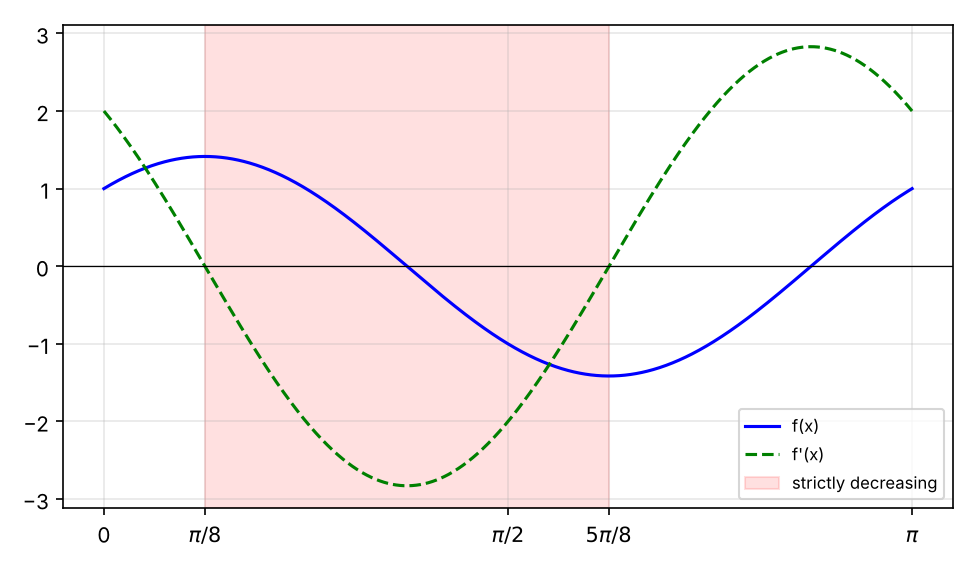
\includegraphics[width=0.70\linewidth]{figs/2.2.23.png}
    \caption{$f(x)=\sin 2x+\cos 2x$ and $f'(x)$}
    \label{fig:decreasing_q23}
\end{figure}

    \item
    \begin{enumerate}[label=(\alph*), leftmargin=1.5em, labelsep=0.5em]
        \item Using elementary row transformations, find the inverse of the matrix
        \begin{align*}
            \begin{bmatrix} 3 & 0 & -1 \\ 2 & 3 & 0 \\ 0 & 4 & 1 \end{bmatrix}
        \end{align*}

        \begin{center}
            \textbf{OR}
        \end{center}

        \item Using matrices, solve the following system of linear equations:
        \begin{align*}
            2x+3y+10z &= 4 \\
            4x-6y+5z &= 1 \\
            6x+9y-20z &= 2
        \end{align*}
    \end{enumerate} \vspace{2pt}
    \textbf{(a) Solution:} From \eqref{eq:EE26BTECH11225-rowops}, apply row operations to $[A\,|\,I]$:
\begin{align}
    [A|I] &= \left[\begin{array}{ccc|ccc} 3 & 0 & -1 & 1 & 0 & 0 \\ 2 & 3 & 0 & 0 & 1 & 0 \\ 0 & 4 & 1 & 0 & 0 & 1 \end{array}\right] \\
    \xrightarrow{R_1\to R_1-R_2}\; &\left[\begin{array}{ccc|ccc} 1 & -3 & -1 & 1 & -1 & 0 \\ 2 & 3 & 0 & 0 & 1 & 0 \\ 0 & 4 & 1 & 0 & 0 & 1 \end{array}\right] \\
    \xrightarrow{R_2\to R_2-2R_1}\; &\left[\begin{array}{ccc|ccc} 1 & -3 & -1 & 1 & -1 & 0 \\ 0 & 9 & 2 & -2 & 3 & 0 \\ 0 & 4 & 1 & 0 & 0 & 1 \end{array}\right] \\
    \xrightarrow{R_2\to R_2-2R_3}\; &\left[\begin{array}{ccc|ccc} 1 & -3 & -1 & 1 & -1 & 0 \\ 0 & 1 & 0 & -2 & 3 & -2 \\ 0 & 4 & 1 & 0 & 0 & 1 \end{array}\right] \\
    \xrightarrow{R_1\to R_1+3R_2}\; &\left[\begin{array}{ccc|ccc} 1 & 0 & -1 & -5 & 8 & -6 \\ 0 & 1 & 0 & -2 & 3 & -2 \\ 0 & 4 & 1 & 0 & 0 & 1 \end{array}\right] \\
    \xrightarrow{R_3\to R_3-4R_2}\; &\left[\begin{array}{ccc|ccc} 1 & 0 & -1 & -5 & 8 & -6 \\ 0 & 1 & 0 & -2 & 3 & -2 \\ 0 & 0 & 1 & 8 & -12 & 9 \end{array}\right] \\
    \xrightarrow{R_1\to R_1+R_3}\; &\left[\begin{array}{ccc|ccc} 1 & 0 & 0 & 3 & -4 & 3 \\ 0 & 1 & 0 & -2 & 3 & -2 \\ 0 & 0 & 1 & 8 & -12 & 9 \end{array}\right]
\end{align}
Thus,
\begin{align}
    A^{-1} = \begin{bmatrix} 3 & -4 & 3 \\ -2 & 3 & -2 \\ 8 & -12 & 9 \end{bmatrix}
\end{align}
\textbf{(b) Solution:} Write the system as $A\vec{x}=\vec{b}$ and use Gaussian elimination on $[A\,|\,\vec{b}]$, with the multipliers of \eqref{eq:EE26BTECH11225-gauss-mult}:
\begin{align}
    \big[A\,|\,\vec{b}\big] &= \left[\begin{array}{ccc|c} 2 & 3 & 10 & 4 \\ 4 & -6 & 5 & 1 \\ 6 & 9 & -20 & 2 \end{array}\right] \\
    \xrightarrow[R_3\to R_3-3R_1]{R_2\to R_2-2R_1}\; &\left[\begin{array}{ccc|c} 2 & 3 & 10 & 4 \\ 0 & -12 & -15 & -7 \\ 0 & 0 & -50 & -10 \end{array}\right]
\end{align}
The pivots $2$, $-12$ and $-50$ are all nonzero, so the elimination does not break down and the solution is unique. By back-substitution, from \eqref{eq:EE26BTECH11225-gauss-back},
\begin{align}
    -50z = -10 &\implies z = \frac{1}{5} \\
    -12y - 15\left(\frac{1}{5}\right) = -7 &\implies y = \frac{1}{3} \\
    2x + 3\left(\frac{1}{3}\right) + 10\left(\frac{1}{5}\right) = 4 &\implies x = \frac{1}{2}
\end{align}
\par\noindent\hfill\mbox{\textit{(\ref{eq:EE26BTECH11225-gauss-mult}, \ref{eq:EE26BTECH11225-gauss-back})}}\par
Thus $x = \frac{1}{2}$, $y = \frac{1}{3}$, $z = \frac{1}{5}$. The C program carries out the elimination and back-substitution and checks the residual of the original system:
\begin{lstlisting}[frame=single, basicstyle=\rmfamily, escapeinside={(*@}{@*)}]
(*@\makebox[\dimexpr\linewidth-2\fboxsep-2\fboxrule\relax][c]{codes/2.2.24b.c}@*)
\end{lstlisting}
To see how the cost grows with the size $n$ of the system, a second C program times Gaussian elimination on random $n \times n$ systems and writes the times to a file. Python is used only to plot them in \figref{fig:gauss_time}; the time grows as $n^3$, as in \eqref{eq:EE26BTECH11225-gauss-cost}.
\begin{lstlisting}[frame=single, basicstyle=\rmfamily, escapeinside={(*@}{@*)}]
(*@\makebox[\dimexpr\linewidth-2\fboxsep-2\fboxrule\relax][c]{codes/2.2.24b\_time.c}@*)
\end{lstlisting}
\begin{lstlisting}[frame=single, basicstyle=\rmfamily, escapeinside={(*@}{@*)}]
(*@\makebox[\dimexpr\linewidth-2\fboxsep-2\fboxrule\relax][c]{codes/2.2.24b\_time.py}@*)
\end{lstlisting}
\begin{figure}[H]
    \centering
    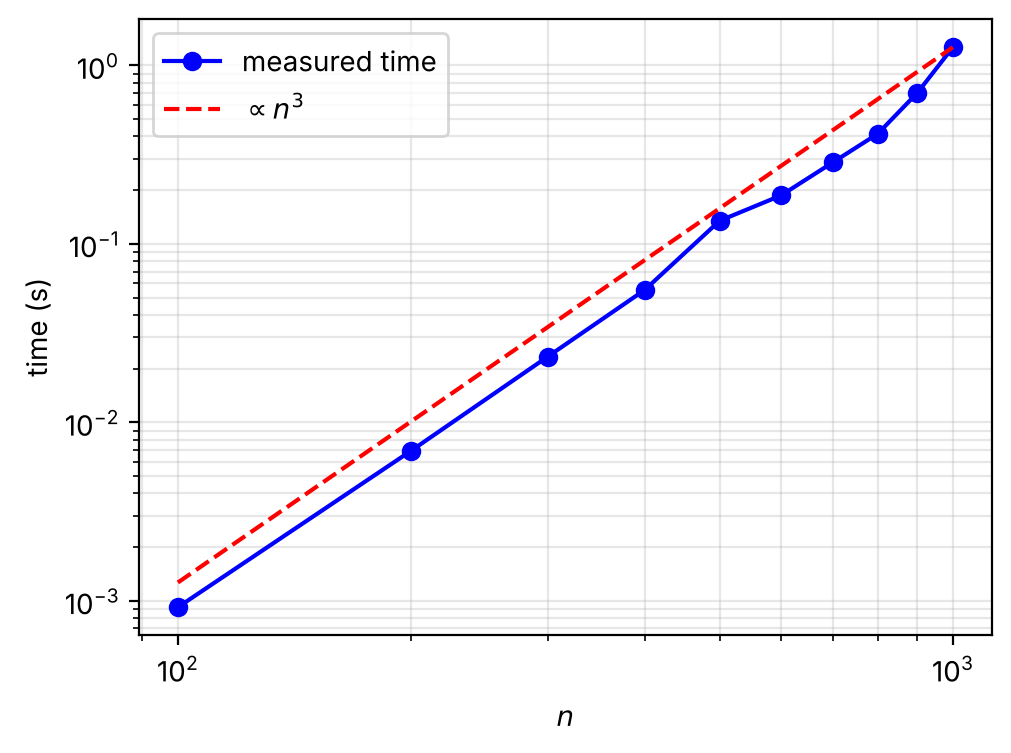
\includegraphics[width=0.65\linewidth]{figs/2.2.24b_time.png}
    \caption{Time of Gaussian elimination against $n$ (log-log), measured by the C program}
    \label{fig:gauss_time}
\end{figure}
The Python program below verifies the inverse in (a) and the solution in (b).
\begin{lstlisting}[frame=single, basicstyle=\rmfamily, escapeinside={(*@}{@*)}]
(*@\makebox[\dimexpr\linewidth-2\fboxsep-2\fboxrule\relax][c]{codes/2.2.24a.py}@*)
\end{lstlisting}

    \item
    \begin{enumerate}[label=(\alph*), leftmargin=1.5em, labelsep=0.5em]
        \item Using integration, find the area of the following region: $\{(x,y) : x^2+y^2\leq 16a^2 \text{ and } y^2\leq 6ax\}$

        \begin{center}
            \textbf{OR}
        \end{center}

        \item Using integration, find the area of triangle $ABC$ bounded by the lines $4x-y+5=0$, $x+y-5=0$ and $x-4y+5=0$.
    \end{enumerate} \vspace{2pt}
    \textbf{(a) Solution:} The circle $x^2+y^2=16a^2$ and the parabola $y^2=6ax$ meet where
\begin{align}
    x^2+6ax-16a^2 = 0 \implies (x+8a)(x-2a) = 0 \implies x = 2a, \quad y = \pm 2\sqrt{3}\,a
\end{align}
Writing both curves as $x$ in terms of $y$, the parabola $x = \frac{y^2}{6a}$ is the left boundary and the circle $x = \sqrt{16a^2-y^2}$ is the right boundary. The region is symmetric about the $x$-axis, so from \eqref{eq:EE26BTECH11225-area-curves-y},
\begin{align}
    \text{Area} &= 2\int_0^{2\sqrt{3}a}\left(\sqrt{16a^2-y^2}-\frac{y^2}{6a}\right)dy
\end{align}
From \eqref{eq:EE26BTECH11225-sqrtint},
\begin{align}
    &= 2\left[\frac{y}{2}\sqrt{16a^2-y^2}+8a^2\sin^{-1}\frac{y}{4a}-\frac{y^3}{18a}\right]_0^{2\sqrt{3}a} \\
    &= 2\left[2\sqrt{3}a^2+\frac{8\pi a^2}{3}-\frac{4\sqrt{3}a^2}{3}\right] \\
    &= \frac{4a^2}{3}\left(4\pi+\sqrt{3}\right)\text{ sq. units}
\end{align}
\textbf{(b) Solution:} Solving the lines pairwise gives the vertices $A(-1,1)$ (lines 1 and 3), $B(0,5)$ (lines 1 and 2) and $C(3,2)$ (lines 2 and 3). Put $t = x+1$. The height of the triangle at $t$ is the upper boundary minus the lower boundary $y=\frac{x+5}{4}$: it is $\frac{15}{4}t$ for $0\le t\le 1$, and $5-\frac{5}{4}t$ for $1\le t\le 4$. With the unit step,
\begin{align}
    h(t) = \frac{15}{4}t - 5(t-1)u(t-1) + \frac{5}{4}(t-4)u(t-4)
\end{align}
From \eqref{eq:EE26BTECH11225-laplace} and \eqref{eq:EE26BTECH11225-laplace-step}, and dividing by $s$ as in \eqref{eq:EE26BTECH11225-laplace-int},
\begin{align}
    H(s) = \frac{1}{s^2}\left(\frac{15}{4} - 5e^{-s} + \frac{5}{4}e^{-4s}\right) \implies \frac{H(s)}{s} = \frac{1}{s^3}\left(\frac{15}{4} - 5e^{-s} + \frac{5}{4}e^{-4s}\right)
\end{align}
Inverting, the area up to $t$ is $\frac{15}{8}t^2 - \frac{5}{2}(t-1)^2u(t-1) + \frac{5}{8}(t-4)^2u(t-4)$, so
\begin{align}
    \text{Area} = \int_0^4 h(t)\,dt = \frac{15}{8}(16) - \frac{5}{2}(9) = 30 - \frac{45}{2} = \frac{15}{2}\text{ sq. units}
\end{align}
This agrees with \eqref{eq:EE26BTECH11225-area-tri}. The following code verifies both parts and generates \figref{fig:area_q25}.
\begin{lstlisting}[frame=single, basicstyle=\rmfamily, escapeinside={(*@}{@*)}]
(*@\makebox[\dimexpr\linewidth-2\fboxsep-2\fboxrule\relax][c]{codes/2.2.25.py}@*)
\end{lstlisting}
\begin{figure}[H]
    \centering
    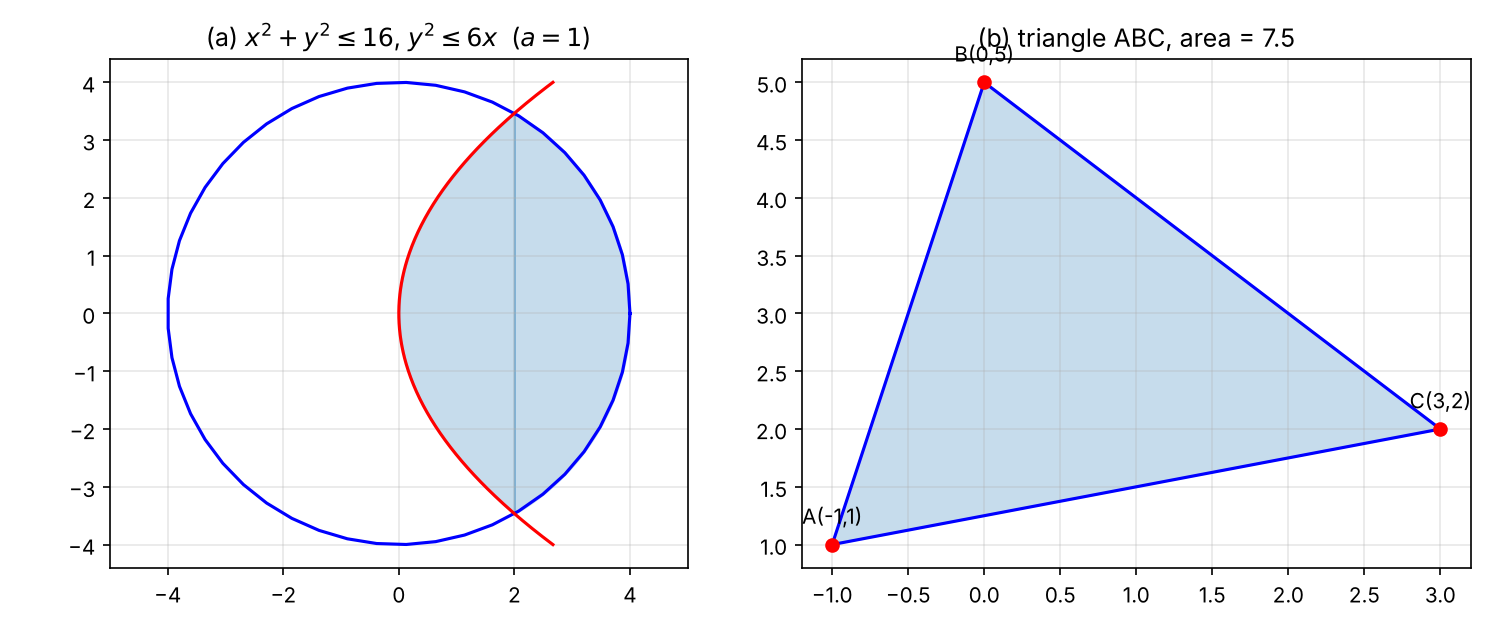
\includegraphics[width=0.95\linewidth]{figs/2.2.25.png}
    \caption{(a) Region inside the circle and the parabola ($a=1$); (b) triangle $ABC$}
    \label{fig:area_q25}
\end{figure}

    \item A company manufactures two types of novelty souvenirs made of plywood. Souvenirs of type A require 5 minutes each for cutting and 10 minutes each for assembling. Souvenirs of type B require 8 minutes each for cutting and 8 minutes each for assembling. There are 3 hours 20 minutes available for cutting and 4 hours for assembling. The profit for type A souvenirs is \rupee 100 each and for type B souvenirs, profit is \rupee 120 each. How many souvenirs of each type should the company manufacture in order to maximise the profit? Formulate the problem as a LPP and then solve it graphically.

\solution Let the company make $x$ souvenirs of type A and $y$ of type B. The available times are $3\text{ h }20\text{ min} = 200$ minutes for cutting and $4\text{ h} = 240$ minutes for assembling. From \eqref{eq:EE26BTECH11225-lpp}:
\begin{align}
    \max Z = 100x+120y \quad\text{s.t.}\quad 5x+8y &\leq 200 \\
    10x+8y &\leq 240 \\
    x,\,y &\geq 0
\end{align}
The corner points of the feasible region are $O(0,0)$, $(24,0)$, $(8,20)$ (where $5x+8y=200$ meets $10x+8y=240$) and $(0,25)$:
\begin{center}
\begin{tabular}{|c|c|}
    \hline
    \textbf{Corner point} & $Z = 100x+120y$ \\ \hline
    $(0,0)$ & $0$ \\ \hline
    $(24,0)$ & $2400$ \\ \hline
    $(8,20)$ & $3200$ \\ \hline
    $(0,25)$ & $3000$ \\ \hline
\end{tabular}
\end{center}
The maximum profit is \rupee 3200, obtained by making $8$ souvenirs of type A and $20$ souvenirs of type B. The following code finds the corner points, checks the result with a linear-programming solver and plots \figref{fig:lpp_q26}.
\begin{lstlisting}[frame=single, basicstyle=\rmfamily, escapeinside={(*@}{@*)}]
(*@\makebox[\dimexpr\linewidth-2\fboxsep-2\fboxrule\relax][c]{codes/2.2.26.py}@*)
\end{lstlisting}
\begin{figure}[H]
    \centering
    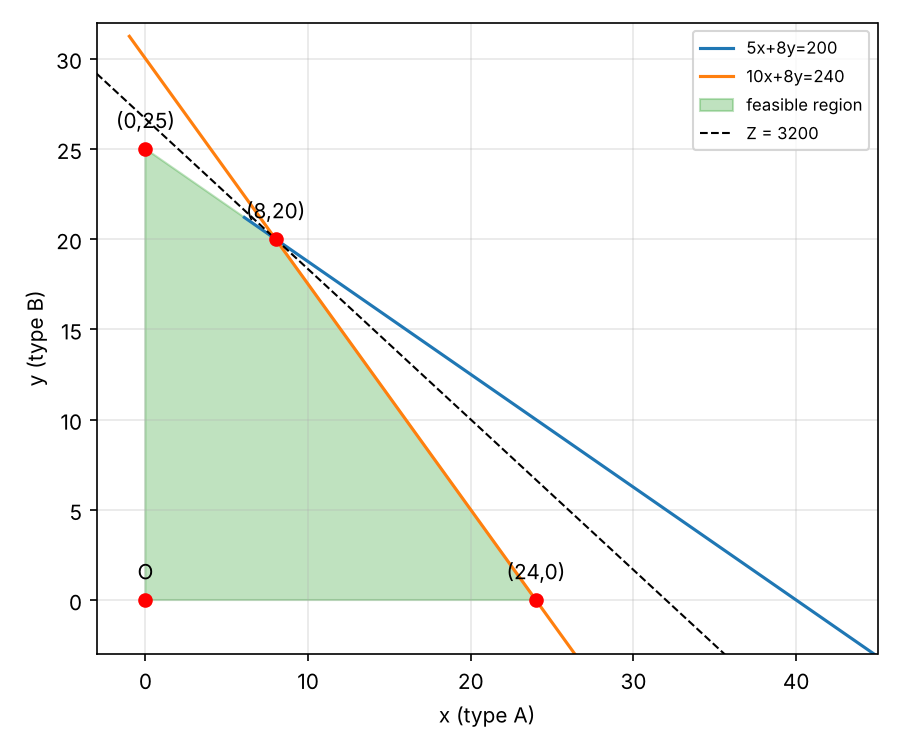
\includegraphics[width=0.70\linewidth]{figs/2.2.26.png}
    \caption{Feasible region and the optimum at $(8,20)$}
    \label{fig:lpp_q26}
\end{figure}

    \item
    \begin{enumerate}[label=(\alph*), leftmargin=1.5em, labelsep=0.5em]
        \item Find the vector equation of the line passing through $(2,1,-1)$ and parallel to the line $\vec{r} = (\hat{i}+\hat{j}) + \lambda(2\hat{i}-\hat{j}+\hat{k})$. Also, find the distance between these two lines.

        \begin{center}
            \textbf{OR}
        \end{center}

        \item Find the coordinates of the foot $Q$ of the perpendicular drawn from the point $P(1,3,4)$ to the plane $2x-y+z+3=0$. Find the distance $PQ$ and the image of $P$ treating the plane as a mirror.
    \end{enumerate} \vspace{2pt}
    \textbf{(a) Solution:} The required line has the same direction $\vec{b} = \myvec{2\\-1\\1}$ and passes through $\vec{a}_2 = \myvec{2\\1\\-1}$:
\begin{align}
    \vec{r} = (2\hat{i}+\hat{j}-\hat{k}) + \mu(2\hat{i}-\hat{j}+\hat{k})
\end{align}
With $\vec{a}_1 = \myvec{1\\1\\0}$, $\vec{a}_2-\vec{a}_1 = \myvec{1\\0\\-1}$ and
\begin{align}
    (\vec{a}_2-\vec{a}_1)\times\vec{b} = \myvec{0\cdot1-(-1)(-1) \\ (-1)(2)-1\cdot1 \\ 1\cdot(-1)-0\cdot2} = \myvec{-1 \\ -3 \\ -1}
\end{align}
From \eqref{eq:EE26BTECH11225-distance-lines}:
\begin{align}
    d = \frac{\sqrt{1+9+1}}{\sqrt{4+1+1}} = \sqrt{\frac{11}{6}} \approx 1.354\text{ units}
\end{align}
\textbf{(b) Solution:} The normal of the plane is $\vec{n} = \myvec{2\\-1\\1}$ and $c=-3$. From \eqref{eq:EE26BTECH11225-foot}:
\begin{align}
    t = \frac{-3-(2-3+4)}{4+1+1} = \frac{-6}{6} = -1
\end{align}
\begin{align}
    \vec{Q} &= \myvec{1\\3\\4} - \myvec{2\\-1\\1} = \myvec{-1\\4\\3} \\
    PQ &= |t|\,\|\vec{n}\| = \sqrt{6} \\
    \vec{P}' &= \vec{P}+2t\vec{n} = \myvec{1\\3\\4} - 2\myvec{2\\-1\\1} = \myvec{-3\\5\\2}
\end{align}
Thus $Q(-1,4,3)$, $PQ=\sqrt{6}$ and the image of $P$ is $P'(-3,5,2)$. The following code verifies both parts and generates \figref{fig:lines3d_q27}.
\begin{lstlisting}[frame=single, basicstyle=\rmfamily, escapeinside={(*@}{@*)}]
(*@\makebox[\dimexpr\linewidth-2\fboxsep-2\fboxrule\relax][c]{codes/2.2.27.py}@*)
\end{lstlisting}
\begin{figure}[H]
    \centering
    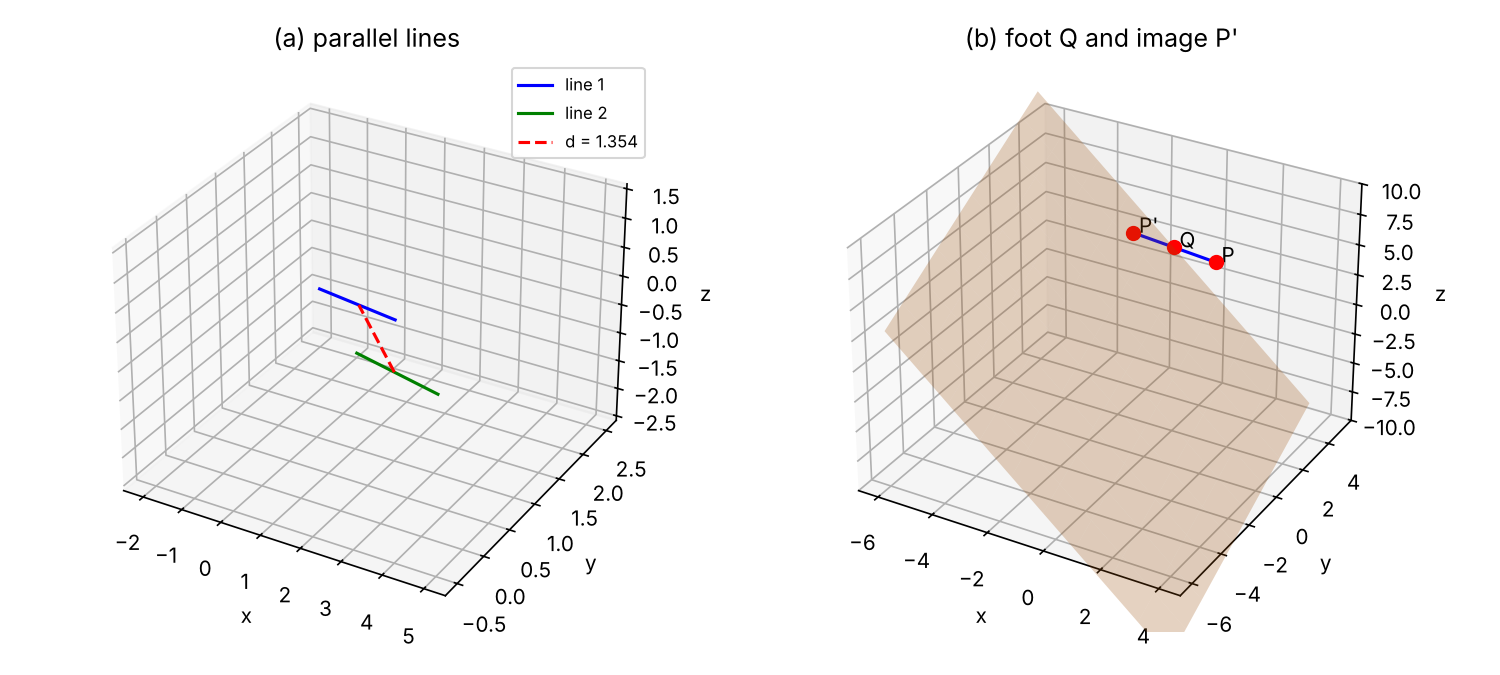
\includegraphics[width=0.95\linewidth]{figs/2.2.27.png}
    \caption{(a) The two parallel lines; (b) foot $Q$ and image $P'$ of $P$}
    \label{fig:lines3d_q27}
\end{figure}

    \item A card from a pack of 52 playing cards is lost. From the remaining cards of the pack, two cards are drawn at random (without replacement) and both are found to be spades. Find the probability of the lost card being a spade.

\solution Let $L = 1$ if the lost card is a spade and $L = 0$ otherwise, and let $Y$ be the number of spades among the two cards drawn. The joint PMF is $p_{LY}(l,2) = p_L(l)\,p_{Y|L}(2|l)$, with
\begin{align}
    p_L(1) = \frac{1}{4}, \quad p_L(0) = \frac{3}{4}
\end{align}
If a spade is lost, $12$ spades remain among $51$ cards; otherwise $13$ remain:
\begin{align}
    p_{LY}(1,2) = \frac{1}{4}\cdot\frac{12}{51}\cdot\frac{11}{50}, \quad p_{LY}(0,2) = \frac{3}{4}\cdot\frac{13}{51}\cdot\frac{12}{50}
\end{align}
Normalizing over $l$ using \eqref{eq:EE26BTECH11225-pmf}, $p_{L|Y}(1|2) = \dfrac{p_{LY}(1,2)}{p_{LY}(1,2)+p_{LY}(0,2)}$:
\begin{align}
    \Pr\brak{L=1 \mid Y=2} = \frac{132}{132+468} = \frac{11}{50}
\end{align}
The following code verifies the result with exact fractions and a simulation.
\begin{lstlisting}[frame=single, basicstyle=\rmfamily, escapeinside={(*@}{@*)}]
(*@\makebox[\dimexpr\linewidth-2\fboxsep-2\fboxrule\relax][c]{codes/2.2.28.py}@*)
\end{lstlisting}

    \item Prove that the radius of the right circular cylinder of greatest curved surface area which can be inscribed in a given cone is half of that of the cone.

\solution Let the cone have base radius $R$ and height $H$, and let the inscribed cylinder have radius $r$ and height $h$. By similar triangles in the cross-section, from \eqref{eq:EE26BTECH11225-inscribed},
\begin{align}
    \frac{h}{H} = \frac{R-r}{R} \implies h = \frac{H(R-r)}{R}
\end{align}
The curved surface area is
\begin{align}
    S = 2\pi rh = \frac{2\pi H}{R}\left(Rr - r^2\right)
\end{align}
Differentiating,
\begin{align}
    \frac{dS}{dr} &= \frac{2\pi H}{R}(R-2r) = 0 \implies r = \frac{R}{2} \\
    \frac{d^2S}{dr^2} &= -\frac{4\pi H}{R} < 0
\end{align}
So $S$ is maximum at $r=\frac{R}{2}$, i.e. the radius of the cylinder is half the radius of the cone (and its height is $\frac{H}{2}$). Hence proved. The following code verifies the maximum and plots \figref{fig:cylinder_q29}.
\begin{lstlisting}[frame=single, basicstyle=\rmfamily, escapeinside={(*@}{@*)}]
(*@\makebox[\dimexpr\linewidth-2\fboxsep-2\fboxrule\relax][c]{codes/2.2.29.py}@*)
\end{lstlisting}
\begin{figure}[H]
    \centering
    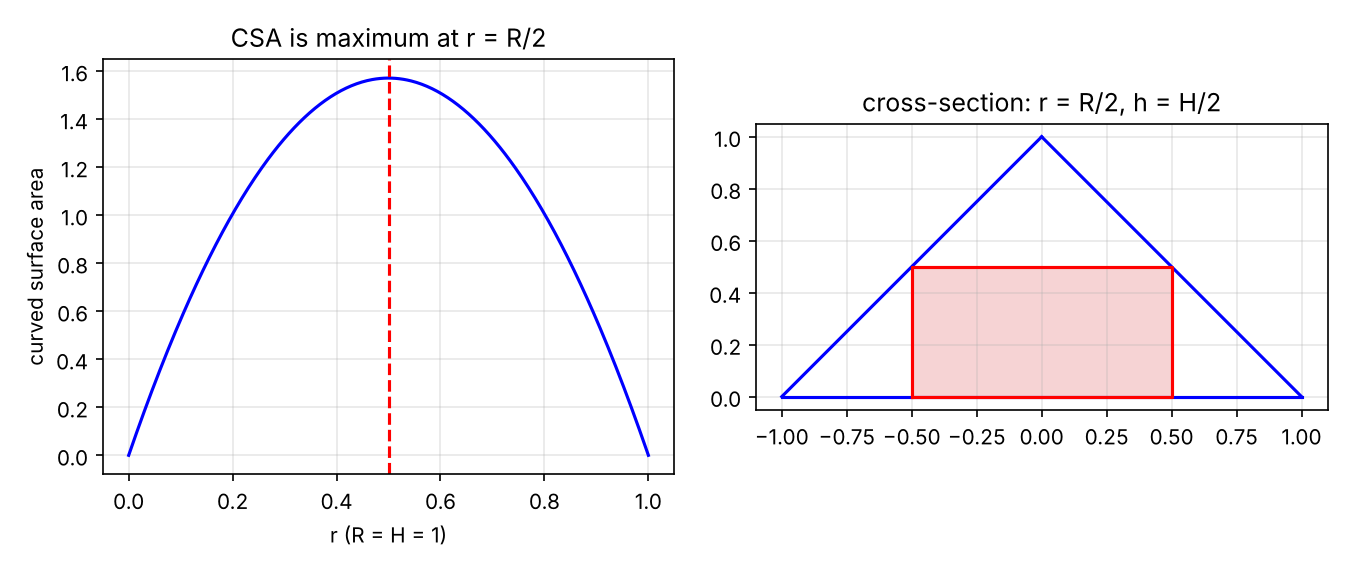
\includegraphics[width=0.95\linewidth]{figs/2.2.29.png}
    \caption{(a) Curved surface area against $r$; (b) the cylinder with $r=R/2$ inside the cone}
    \label{fig:cylinder_q29}
\end{figure}

\end{enumerate}


\end{document}
